\documentclass{article}
\usepackage[utf8]{inputenc}
\usepackage{enumitem}
\usepackage{amssymb}
\usepackage{amsmath}
\usepackage{amsthm}
\usepackage{bm}
\usepackage{hyperref}
\usepackage{geometry}
\geometry{a4paper,scale=0.8}
\usepackage[square,numbers]{natbib}
\bibliographystyle{abbrvnat}
\usepackage{tikz}
\usepackage{tkz-euclide}
\usetikzlibrary{positioning, decorations.markings, arrows, intersections}
\usepackage{nicematrix}
\NiceMatrixOptions{cell-space-top-limit = 4pt}
\NiceMatrixOptions{cell-space-bottom-limit = 4pt}
\usepackage{tcolorbox}
\usepackage{caption, subcaption}
\captionsetup[figure]{labelfont={bf},name={Fig.},labelsep=period}
\captionsetup[table]{labelfont={bf},name={Tab.},labelsep=period}
\setlength\arrayrulewidth{0.7pt}
\usepackage{authblk}
\usepackage{soul}
%\usepackage{showlabels}
\usepackage{multirow}

\newtheorem*{remark}{Remark}
\DeclareMathOperator*{\argmin}{arg\,min}

\newcommand{\mycolorbox}[2]{\colorbox{#1}{$\displaystyle#2$}}
\newcommand{\todo}[1]{\textcolor{blue}{\fbox{\textbf{TODO: #1}}}}
\newcommand{\mycomment}[1]{\noindent\textcolor{orange}{\underline{\textsf{\textbf{#1}}}}}
\newcommand{\todobox}[1]{
    \begin{tcolorbox}[title=TODO list, colback=blue!10, colframe=blue]
        #1
    \end{tcolorbox}
}


\title{APPM report - Draft}
\author[1]{R. Hiptmair}
\author[1]{T.W. Yu}
\author[2]{R. Fuchs}
\affil[1]{Seminar for Applied Mathematics , ETH Z\"{u}rich}
\affil[2]{IET Institut für Energietechnik, OST}
\date{}

\begin{document}
\maketitle

\section*{Abstract}
% \todo{polish the abstract}

We elaborate a numerical method for a three-dimensional hydrodynamic multi-species plasma
model which boils down to an extended Euler-Maxwell system. Our method is inspired by and
extends the one-dimensional scheme from $[$P.~Degond, F.~Deluzet, and D.~Savelief,
\emph{Numerical approximation of the Euler-Maxwell model in the quasineutral limit}, Journal of
Computational Physics, 231 (4), pp.~1917--1946, 2012$]$. It can cope with large variations
of the so-called Debye length $\lambda_D$ and is robust in the quasi-neutral
singular-perturbation limit $\lambda_D\to 0$, because it enjoys an
\emph{asymptotic-preserving} (AP) property in the sense that in the sense that the limit
$\lambda_D\to 0$ of the scheme yields a viable discretization for the continuous limit
model. The key ingredients of our approach are (i) a discretization of Maxwell's equations
based on primal and dual meshes in the spirit of \emph{discrete exterior calculus} (DEC)
also known the finite integration technique (FIT), (ii) a finite volume method (FVM) for
the fluid equations on the dual mesh, (iii) \emph{mixed implicit-explicit timestepping},
(iv) special no-flux and contact boundary conditions at an outer cut-off boundary, and (v)
additional \emph{stabilization} in the non-conducting region outside the plasma domain
based on direct enforcement of Gauss' law. Numerical tests provide strong evidence
confirming the AP property of the new method.

%The scheme is designed to be AP as $\lambda_D \rightarrow 0$ and this is validated through numerical experiments. Besides, if the electromagnetic fields have to be modelled in an non-conducting region beyond the plasma domain, additional stabilization to accommodate Gauss's law is necessary.

%\noindent\textbf{A short version:}

%The Debye length $\lambda_D$, as a key characteristic coefficient of plasmas, may range over many orders of magnitude. The induced singularly perturbed problem is a challenge for plasma simulations. Recently so called asymptotic-preserving (AP) schemes, which target such problems, are studied widely. However, in the context of plasma simulations, only AP schemes in one spatial dimension are available. In this work, we construct an AP scheme for Maxwell-Euler equations in three spatial dimensions based on primal-dual meshes and the finite integration technique (FIT) for Maxwell's equations coupled with the finite volume method (FVM) for the fluid equations. Besides, issues like boundary treatment and stabilization in non-conducting regions are tackled. The AP property is verified numerically. We expect this new discretization approach is particularly suited for problems involving multiple scales of the Debye length, e.g. electric arcs.


%\noindent\textbf{A long version:}

%{\color{red}
%A key coefficient characterizing plasmas is the so-called Debye length $\lambda_D$, whose magnitude indicates to what extent net electric charges deviate from zero. It may range over many orders of magnitude: If $\lambda_D = \mathcal{O}(1)$ we face the non-neutral regime, while for $\lambda_D\to 0$ the plasma becomes quasi-neutral. A singularly perturbed problem arises from the $\lambda_D\to 0$ limit, which leads to peculiar issues in numerical algorithms when both regimes coexist, for instance, in the fringes of electric arcs and near electrodes. It is desired to design numerical schemes that are \emph{robust} for arbitrary $\lambda_D$. More precisely, they should be \emph{asymptotic-preserving} (AP), in the sense that the limit $\lambda_D\to 0$ of the scheme yields a viable discretization for the continuous limit model.

%An asymptotic-preserving scheme for single- and multi-fluid Euler-Maxwell system was proposed by \cite{degond_2012} for one spatial dimension. We extend their scheme to three dimensions. The key ingredients are (i) a discretization of Maxwell's equations based on primal and dual meshes in the spirit of discrete exterior calculus (DEC)/the finite integration technique (FIT), (ii) finite volume method (FVM) for the fluid equations on the dual mesh, and (iii) mixed implicit-explicit timestepping. The scheme is designed to be AP as $\lambda_D \rightarrow 0$ and this is validated through numerical experiments. Besides, if the electromagnetic fields have to be modelled in an non-conducting region beyond the plasma domain, additional stabilization to accommodate Gauss's law is necessary.
%}

\section{Introduction}

% \mycomment{Roman: more info from a physical point of view?} R.H. 19.12. Extended paragraph
The starting point for this work was the desire to numerically simulate the formation and
evolution of electric arcs at atmospheric pressures. Following common practise, we rely on
a mathematical description by means of a hydrodynamic multi-species plasma model, which
boils down to an extended Maxwell-Euler system. The arc phenomenon covers a wide range of
plasma regimes and, thus, the design goal was a numerical model capable of dealing
with all of them seamlessly and simultaneously. Thus in this work, as in
\cite{degond_2012}, the focus is on \emph{asymptotic-preserving} (AP) discretization in
the quasi-neutral limit $\lambda \rightarrow 0$, where $\lambda$ is the rescaled Debye
length, see Section \ref{sec:rescaling} for the underlying scaling arguments and
\cite{degond_2012,degond_2017} for a discussion of the importance of the AP property of
numerical plasma models.

Our approach is inspired by \cite{degond_2012}, but goes beyond that work in various directions:
\begin{itemize}
\item We supplement the Maxwell-Euler system by inter-species friction terms.
\item We extend the spatially one-dimensional scheme of \cite{degond_2012} to three
  spatial dimensions using discrete exterior calculus (DEC) to discretize Maxwell's
  equations combined with a low-order finite volume method for Euler's equations.
\item We propose a stabilization in non-conducting regions which is essential for the
  efficacy of our method.
\end{itemize}

We stay close to \cite{degond_2012} in terms of discretization in time employing
semi-implicit time-stepping. We also base our considerations on the model geometry shown
in Fig. \ref{fig:domain_geometry}. We would like to remark that the mesh-based numerical
scheme proposed in this paper can in principle be adapted to geometric situations much
more general than that of Fig. \ref{fig:domain_geometry}. However, one may encounter
subtle problems in defining proper dual meshes as we need it in Section
\ref{sec:mesh-duality}. Thus, for the sake of simplicity of presentation we forgo
geometric generality.

The quasi-neutral limit of the Maxwell-Euler system leads to a singularly perturbed
problem, that is, the limiting PDE system changes its type\footnote{The type of the
  Maxwell-Euler system switches from hyperbolic to mixed for $\lambda_{D}\to 0$}. This
poses a challenge for simulations in settings encompassing different regimes. We remind
that singularly perturbed problems occur in many physical models, e.g., in the case of
vanishing viscosity in the Navier-Stokes equations \cite{Kato_1984}, the
zero-relaxation-limit of kinetic equations \cite{jin_2010}, and the zero-Mach-number limit
of compressible flows \cite{degond_2007, haack_2010}. Throughout, it is essential that
numerical schemes remain valid even if crucial model parameters approach the limit. These
schemes are then said to be \emph{asymptotic-preserving} (AP): Let us assume that we
discretize a parameter($\lambda$)-dependent model $P^\lambda$, which converges to a limit
$P^0$ as $\lambda \rightarrow 0$, by the scheme $P^\lambda_h$ where $h$ denotes some
discretization parameter, e.g., the mesh size. The AP property amounts to uniform
convergence of $P^\lambda_h$ to the $P^\lambda$ as $\lambda\rightarrow0$. Readers are
referred to the illustration by a commuting diagram in \cite[][Fig. 1]{jin_2010} and, more
generally, to the comprehensive reviews \cite{jin_2010, degond_2017} for more details
about AP schemes.

The content of this paper is organized as follows: In Section \ref{sec:plasma-model}, we
give a full description of the underlying equations of the Maxwell-Euler system and its
rescaling procedure. Meanwhile, the boundary conditions in our setting is elaborated. A
reformulation of Maxwell's equations in the non-conducting region is presented. Section
\ref{sec:spatial_discretization} is devoted to the spatial discretization. The concept of
primal-dual meshes is introduced based on which FIT and FVM are utilized. We discuss the
full AP discretization in Section \ref{sec:full-discretization} and do numerical
experiments in Section \ref{sec:numerical_experiment}.

\begin{figure}
    \centering
    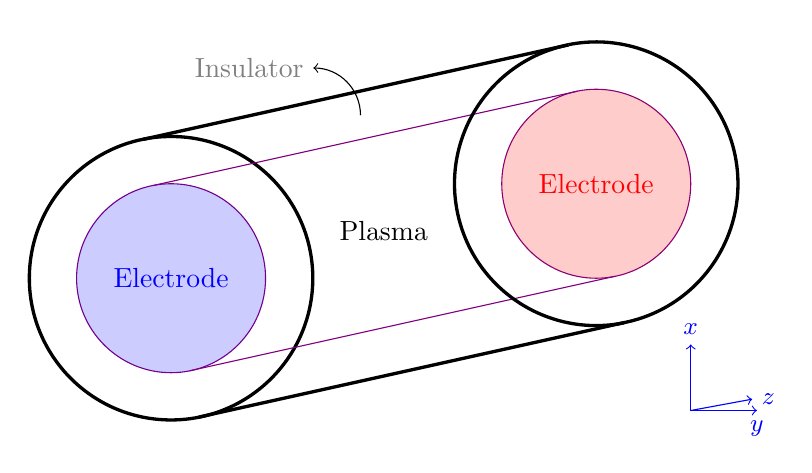
\begin{tikzpicture}[scale=1.2]
    \coordinate (O1) at (0,0);
    \draw[violet] (O1) circle (1) node[blue] {Electrode};
    \fill[blue, opacity=0.2] (O1) circle (1);
    \draw[very thick] (O1) circle (1.5);
    \coordinate (O2) at (4.5,1);
    \draw[violet] (O2) circle (1);
    \node at (O2) {\textcolor{red}{Electrode}};
    \node at (barycentric cs:O1=1,O2=1) {Plasma}; 
    \fill[red, opacity=0.2] (O2) circle (1);
    \coordinate (S1) at ([shift={(-0.196,0.98)}]O1);
    \coordinate (S2) at ([shift={(-0.196,0.98)}]O2);
    \coordinate (P1) at ([shift={(0.196,-0.98)}]O1);
    \coordinate (P2) at ([shift={(0.196,-0.98)}]O2);
    \draw[violet] (S1) -- (S2);
    \draw[violet] (P1) -- (P2);
    \coordinate (SS1) at ([shift={({-0.196*1.5},{0.98*1.5})}]O1);
    \coordinate (SS2) at ([shift={({-0.196*1.5},{0.98*1.5})}]O2);
    \coordinate (PP1) at ([shift={({0.196*1.5},{-0.98*1.5})}]O1);
    \coordinate (PP2) at ([shift={({0.196*1.5},{-0.98*1.5})}]O2);
    \draw[very thick] (SS1) -- (SS2);
    \draw[very thick] (PP1) -- (PP2); 
    \draw[black, very thick] (SS2) arc (101.31:180+101.31:1.5);
    \draw[very thick] (PP2) arc (101.31-180:101.31:1.5);
    \draw[-to] (barycentric cs:SS1=1,SS2=1,S1=1,S2=1) to[out=90,in=0] ([shift={(-0.5,0.5)}]barycentric cs:SS1=1,SS2=1,S1=1,S2=1) node[left, gray] {Insulator};
    \begin{scope}[shift={(5.5,-1.4)}]
    \draw[blue, -to] (0,0) -- (0.65,0.12) node[right]{\small $z$};
    \draw[blue, -to] (0,0) -- (0,0.7) node[above]{\small $x$};
    \draw[blue, -to] (0,0) -- (0.7,0) node[below]{\small $y$};
    \end{scope}
    \end{tikzpicture}
    \caption{The special geometric setting suggested by the simulation of electric arcs,
      for which we discuss the new method.}
\label{fig:domain_geometry}
\end{figure}

\section{Plasma model} \label{sec:plasma-model}

\subsection{The Maxwell-Euler System}

Plasmas consist of electrically charged and (possibly) neutral particle species and we
suppose that they can be treated as continua (fluids). That is, they may be described by the
Navier-Stokes equations augmented with source terms for species generation (ionization,
recombination), forces (Lorentz force and interspecies friction), and energy (thermal
relaxation among species, radiative heat transfer, Ohmic heating). For more details on
fluid models of plasmas, see \cite{chen2016, remi_2014}.

The electromagnetic effects in plasmas are governed by Maxwell's equations:
\begin{subequations}
\begin{align}
    \partial_t \mathbf{B} + \nabla \times \mathbf{E} &= 0, \label{equ:maxwell_faraday} \\ 
    \partial_t \mathbf{D} - \nabla \times \mathbf{H} &= -\mathbf{J}, \label{equ:maxwell_ampere} \\
    \nabla \cdot \mathbf{B} &= 0,  \label{equ:maxwell_gauss_B}\\
    \nabla \cdot \mathbf{D} &= \rho, \label{equ:maxwell_gauss_D}
\end{align}
\end{subequations}
where the involved quantities\footnote{SI units in square brackets.} are the magnetic flux
density $\mathbf{B}[\frac{\text{Wb}}{\text{m}^2}]$, the electric field
$\mathbf{E}[\frac{\text{V}}{\text{m}}]$, the electric displacement field
$\mathbf{D}[\frac{\text{C}}{\text{m}^2}]$, the magnetic field
$\mathbf{H}[\frac{\text{A}}{\text{m}}]$, the electric current density
$\mathbf{J}[\frac{\text{A}}{\text{m}^2}]$ and the electric charge density
$\rho[\frac{\text{C}}{\text{m}^3}]$. These equations are known as Faraday's law
(\ref{equ:maxwell_faraday}), Amp\`{e}re's law (\ref{equ:maxwell_ampere}), Gauss's law for
magnetism (\ref{equ:maxwell_gauss_B}) and Gauss's law for electric field
(\ref{equ:maxwell_gauss_D}). For simplicity, we only consider isotropic and homogeneous
media. Namely, we rely on linear constitutive relations (material laws):
\begin{equation} \label{equ:material_law}
    \mathbf{D} = \epsilon \mathbf{E}\quad,\quad\mathbf{B} = \mu\mathbf{H}, 
\end{equation}
where $\epsilon[\frac{\text{F}}{\text{m}}]$ and $\mu[\frac{\text{N}}{\text{A}^{2}}]$ are
the permittivity and permeability and assumed to be constant. By taking the time
derivative of (\ref{equ:maxwell_gauss_D}) and the divergence of
(\ref{equ:maxwell_ampere}), it is easy to see that (\ref{equ:maxwell_ampere}) and
(\ref{equ:maxwell_gauss_D}) implies the charge conservation
\begin{equation} \label{equ:charge_continuity}
    \partial_t\rho + \nabla \cdot \mathbf{J} = 0.
\end{equation}
Besides, by taking the divergence of equations (\ref{equ:maxwell_faraday}) and
(\ref{equ:maxwell_ampere}) together with the relation (\ref{equ:charge_continuity}), it is
possible to verify that Gauss's laws (\ref{equ:maxwell_gauss_B})
(\ref{equ:maxwell_gauss_D}) are consequences of (\ref{equ:maxwell_faraday}) and
(\ref{equ:maxwell_ampere}) provided that (\ref{equ:maxwell_gauss_B})
(\ref{equ:maxwell_gauss_D}) are satisfied at initial time. In other words, Gauss's laws
(\ref{equ:maxwell_gauss_B}) (\ref{equ:maxwell_gauss_D}) can be thought of as initial
conditions.

We model each species in the plasma as a compressible fluid through a set of \emph{Euler
  equations} augmented by electromagnetic forces as well as other processes,
e.g. collisions and recombination:
\begin{align} \label{equ:euler_}
    \partial_t
    \begin{pmatrix}
    n_* \\
    m_*n_* \mathbf{u}_* \\
    m_*n_* e_*
    \end{pmatrix}
    + \nabla \cdot
    \begin{pmatrix}
    n_* \mathbf{u}_* \\
    m_*n_* \mathbf{u}_* \otimes \mathbf{u}_* + p_*\mathbb{I} \\
    m_*n_* h_* \mathbf{u}_*
    \end{pmatrix}
    =
    \begin{pmatrix}
    0 \\
    q_*n_*(\mathbf{E} + \mathbf{u}_* \times \mathbf{B}) \\
    \mathbf{J}_* \cdot \mathbf{E}
    \end{pmatrix}
    +
    \begin{pmatrix}
    \Gamma_* \\
    \mathbf{R}_* \\
    Q_*
    \end{pmatrix}.
\end{align}
The subscript $*\in \{e, i, \cdots\}$ labels electrons, ions or other species. The
involved fluid quantities are: number density $n_*[\frac{1}{\text{m}^3}]$, particle mass
$m_*[\text{kg}]$, electric charge $q_*[\text{C}]$, velocity
$\mathbf{u}_*[\frac{\text{m}}{\text{s}}]$, pressure $p_*[\frac{\text{N}}{\text{m}^2}]$,
specific total energy
$e_* := \frac{1}{2}|\mathbf{u}_*|^2 + \frac{p_*}{m_*n_*(\gamma -
  1)}[\frac{\text{J}}{\text{kg}}]$, specific total enthalpy
$h_* := e_* + \frac{p_*}{m_*n_*}[\frac{\text{J}}{\text{kg}}]$ and current density
$\mathbf{J}_* := q_*n_*\mathbf{u}_*[\frac{\text{A}}{\text{m}^2}]$. All species are
assumed to be ideal gases with heat capacity ratio $\gamma=5/3$ for monatomic gases. The
left-hand side of the equations describes the convection of plasma fluids. The first term
at the right-hand side takes into account the Lorentz force in the momentum equation and
Joule heating in the energy equation. $\Gamma_*, \mathbf{R}_*, Q_*$ are generic terms due
to effects of inter-species collision, ionization, recombination, etc.

Combining the two sets of equations (\ref{equ:maxwell_faraday}) to
(\ref{equ:maxwell_gauss_D}) and (\ref{equ:euler_}) leads to the governing equations for a
multi-species plasma model. The coupling of the two subsystems is due to the fact that the
flow of charged particles induces electric currents:
\begin{equation} \label{equ:maxwell_euler_coupling}
    \rho = \sum_* q_*n_*\;, \quad \mathbf{J} = \sum_* q_*n_*\mathbf{u}_*. 
\end{equation}

\begin{remark}
  \label{rem:coll}
  For the sake of simplicity, we only consider ion-electron collision in this work, but
extension to more species is straightforward. Such collisions can be well modelled by
friction terms, for instance \citep[][Sec. 5.6.2]{chen2016}
\begin{equation} \label{equ:collision}
    \mathbf{R}_{e}^{\text{coll}} = \frac{\pi Ze^4m_e^{1/2}}{(4\pi\epsilon)^2(k_BT_e)^{3/2}}\text{ln}\Lambda n_en_i(\mathbf{u}_i - \mathbf{u}_e) = - \mathbf{R}_{i}^{\text{coll}},  
\end{equation}
which is the collision force acting on electrons. ln$\Lambda$ is called the \emph{Coulomb
  logarithm} and is usually taken as a constant \cite{chen2016}. Because of the
conservation of momentum, the collision term for ions $\mathbf{R}_{i}^{\text{coll}}$ is
nothing but the negative of $\mathbf{R}_{e}^{\text{coll}}$. In this work, the other
effects, e.g. ionization and recombination, are not considered. For full details about the
modeling of these physical processes, readers are referred to
\cite[][Sec. 3.2]{fuchs_2021}.
\end{remark}

\subsection{Rescaling}
\label{sec:rescaling}
% In rescaling, variables in equations are replaced by the ratio of original quantities and constant reference quantities, which transforms the system into dimensionless form. In this part, the rescaling procedure mostly follows that of \cite[][Sec. 2.2]{degond_2017}.

We arrive at non-dimensional equations by following the rescaling procedure of
\cite[][Sec. 2.2]{degond_2017}.  First, a reference value for each quantity is
prescribed. We define $\overline{x}$ and $\overline{t}$ as space and time scale of
interest, by which the reference velocity $\overline{v}$ is defined as
$\overline{x}/\overline{t}$. The typical magnitudes of electromagnetic fields are
$\overline{E}$ and $\overline{B}$. The reference magnitudes of fluid quantities are
denoted by $\overline{u}$ for plasma drift velocity, $\overline{n}$ for plasma number
density, $\overline{T}$ for plasma temperature. On top of that, the reference pressure is
set to $\overline{n}k_B\overline{T}$ with $k_B$ being the Boltzmann constant; the
reference value for the specific total energy and enthalpy is set to
$\overline{u}^2$. Also taking into account the physical constants, i.e. the reference
permittivity $\overline{\epsilon}$, the reference permeability $\overline{\mu}$, the light
speed $c^2 = (\overline{\epsilon}\overline{\mu})^{-1}$, Boltzmann constant $k_B$, the
elementary charge $e$, and ion mass $m_i$, we introduce the following dimensionless
parameters:
\begin{align*} 
  \xi &:= \frac{\overline{v}}{c} \text{ the velocity of interest \emph{w.r.t.}\footnotemark[1] the light speed}, &\\
  \zeta &:= \frac{\overline{u}}{\overline{v}} \text{ the plasma velocity \emph{w.r.t.} the speed of interest}, &\\
  M &:= \frac{\overline{u}}{v_i^{\text{th}}} \text{ the plasma drift velocity \emph{w.r.t.} the thermal speed of ions, where } v_i^{\text{th}} := \left(\frac{k_B \overline{T}}{m_i}\right)^{1/2}, &\\
  \eta &:= \frac{e\overline{E}\overline{x}}{m_i\overline{u}^2} \text{ the electric energy \emph{w.r.t.} the kinetic energy of ions}, &\\
  \beta &:= \frac{\overline{v}\overline{B}}{\overline{E}} \text{ the induced electric field \emph{w.r.t.} the total electric field}, &\\
  \lambda &:= \frac{\lambda_D}{\overline{x}} \text{ the dimensionless Debye length, where }\lambda_D := \left(\frac{\epsilon k_B\overline{T}}{e^2\overline{n}}\right)^{1/2}, &\\
  \varepsilon_*^2 &:= \frac{m_*}{m_i} \text{ the species mass \emph{w.r.t.} the ion mass},\ \  * \in \{i,e,\cdots\}, &\\
  g &:= \frac{1}{\overline{n}\lambda_D^3} \text{ the plasma parameter\footnotemark[2]}.&
\end{align*}
\footnotetext[1]{Abbreviation of \emph{with respect to}.}
\footnotetext[2]{It is basically the reciprocal of the number of particles per Debye sphere, see \cite[][Sec. 1.1]{gibbon2020}. Classical plasma theory assumes $g \ll 1$.} 

By abuse of notation, the rescaled variables share the same notation as before
rescaling. We neglect ionization and recombination but retain collision terms,
i.e. $\Gamma_* = 0, \mathbf{R}_* = \mathbf{R}_*^\text{coll}, Q_* = Q_*^\text{coll}$ in
(\ref{equ:euler_}). The rescaled Euler-Maxwell system is
\begin{subequations}
\begin{align}
  \beta \partial_t \mathbf{B} + \nabla \times \mathbf{E} &= 0, \label{equ:maxwell_faraday_rescalling} \\ 
  \lambda^2 \partial_t \mathbf{D} - \frac{\beta \lambda^2}{\xi^2}\nabla \times \mathbf{H} &= - \frac{\zeta}{\eta M^2}\mathbf{J}, \label{equ:maxwell_ampere_rescalling} \\
  \nabla \cdot \mathbf{B} &= 0,  \label{equ:maxwell_gauss_B_rescalling}\\
  \lambda^2 \eta M^2 \nabla \cdot \mathbf{D} &= \rho, \label{equ:maxwell_gauss_D_rescalling} \\
  \partial_t
    \begin{pmatrix}
    n_* \\
    n_* \mathbf{u}_* \\
    n_* e_*
    \end{pmatrix}
    + \nabla \cdot
    \begin{pmatrix}
    \zeta n_* \mathbf{u}_* \\
    \zeta n_* \mathbf{u}_* \otimes \mathbf{u}_* + \zeta M^{-2} \varepsilon_*^{-2} p_*\mathbb{I} \\
    \zeta n_* h_* \mathbf{u}_*
    \end{pmatrix}
    &=
    \begin{pmatrix}
    0 \\
    \eta \zeta \varepsilon_*^{-2} q_* n_*\mathbf{E} + \eta \zeta^2 \beta \varepsilon_*^{-2} q_* n_* \mathbf{u}_* \times \mathbf{B} \\
    \zeta \eta \varepsilon_*^{-2} \mathbf{J}_* \cdot \mathbf{E}
    \end{pmatrix} +
    \begin{pmatrix}
    0 \\
    \varepsilon_*^{-2}\mathbf{R}_*^{\text{coll}} \\
    \varepsilon_*^{-2}Q_*^{\text{coll}} \\
    \end{pmatrix}, \label{equ:euler_rescalling}
\end{align}
\end{subequations}
where the equation of state becomes
$e_* = \frac{1}{2}|\mathbf{u_*}|^2 + M^{-2}\frac{p_*}{\epsilon^2_* n_* (\gamma - 1)}$ and
$h_* = e_* + M^{-2}\frac{p_*}{\epsilon^2_* n_*}$. For a fully-ionized gas, we have the
original expression of $\mathbf{R}_*^{\text{coll}}$ in (\ref{equ:collision}), and its
rescaled expression becomes
\begin{equation}
    \mathbf{R}_i^{\text{coll}} = \frac{Z\text{ln}\Lambda}{16\pi}g\lambda^{-1}M^{-1}\varepsilon_en_en_i(\mathbf{u}_i - \mathbf{u}_e). \label{equ:rescaling_friction}
\end{equation}

Assumptions can be made to reduce the number of dimensionless parameters. Following
\cite[][Sec. 2.2]{degond_2017}, the reference speed $\overline{v}$ is of the same scale as
the plasma speed $\overline{u}$ and the thermal speed $v_i^{\text{th}}$ whereas it is much
smaller than the light speed $c$. Also, it is assumed that $\eta$ and $\beta$ are of order
one and $\xi$ has the same magnitude as $\lambda$.

\begin{remark}
Special treatment is needed for the collision term. One could argue that the occurrence of
$\lambda^{-1}$ in (\ref{equ:rescaling_friction}) could lead to singular perturbation of
the Euler system as $\lambda \rightarrow 0$. However, the validity of such a collision
model is doubtful when $\lambda \rightarrow 0$. From the physical viewpoint, the shielding
effect characterized by the rescaled Debye length $\lambda$ limits the impact parameters
to values $\sim\lambda$. The $\lambda \rightarrow 0$ limit implies that the collisions
happen on the atomic length scale, in which quantum-mechanical effects must be taken into
account \cite[][pp. 144-148]{frank_1972}. Therefore, we eliminate the perturbation
parameter in the friction term by assuming $g \sim \lambda$ and keep the prefactor
$\alpha^{\text{coll}}$ of the collision term constant throughout the simulation.

The case when there is an asymptotic parameter in the denominator of the friction term is
of interest, too. This situation is known as relaxation limit, see \cite{peng_2011,
  wasiolek_2016, Li_2021, Chen_2000}.
\end{remark}

In summary, we make the following choices \cite[][sec 2.2]{degond_2017}
\begin{align*}
    \xi \sim g \sim \lambda \in [0,1], \ \ \ \zeta \sim M \sim \eta \sim \beta \sim \mathcal{O}(1).
\end{align*}
Assuming this behavior of the dimensionless parameters, the rescaled Euler-Maxwell system
is simplified to a system of PDEs with the dimensionless \emph{Debye length} $\lambda$ as
single parameter, whose value may tend to zero:
\begin{subequations}
  \label{resc}
\begin{align}
    \partial_t \mathbf{B} + \nabla \times \mathbf{E} &= 0, \label{equ:maxwell_faraday_rescaled} \\ 
    \colorbox{yellow!30}{$\displaystyle\lambda^2$} \partial_t \mathbf{D} - \nabla \times \mathbf{H} &= - \mathbf{J}, \label{equ:maxwell_ampere_rescaled} \\
    \nabla \cdot \mathbf{B} &= 0,  \label{equ:maxwell_gauss_B_rescaled}\\
    \colorbox{yellow!30}{$\displaystyle\lambda^2$} \nabla \cdot \mathbf{D} &= \rho, \label{equ:maxwell_gauss_D_rescaled} \\
    \partial_t
    \begin{pmatrix}
    n_* \\
    n_* \mathbf{u}_* \\
    n_* e_*
    \end{pmatrix}
    + \nabla \cdot
    \begin{pmatrix}
    n_* \mathbf{u}_* \\
    n_* \mathbf{u}_* \otimes \mathbf{u}_* + \varepsilon_*^{-2} p_*\mathbb{I} \\
    n_* h_* \mathbf{u}_*
    \end{pmatrix}
    &=
    \begin{pmatrix}
    0 \\
    \varepsilon_*^{-2} q_* n_* (\mathbf{E} + \mathbf{u}_* \times \mathbf{B}) \\
    \varepsilon_*^{-2} \mathbf{J}_* \cdot \mathbf{E}
    \end{pmatrix}+
    \begin{pmatrix}
    0 \\
    \varepsilon_*^{-2}\mathbf{R}_*^{\text{coll}} \\
    \varepsilon_*^{-2}Q_*^{\text{coll}} 
    \end{pmatrix}, \label{equ:euler_rescaled}
\end{align}
with the equation of state
$e_* = \frac{1}{2}|\mathbf{u_*}|^2 + \frac{p_*}{\varepsilon^2_* n_* (\gamma - 1)}$ and
$h_* = e_* + \frac{p_*}{\varepsilon^2_* n_*}$. For a fully-ionized gas with only ions and
electrons,
\begin{equation} \label{equ:collision_rescaled} 
    \mathbf{R}_i^{\text{coll}} = \alpha^{\text{coll}}n_en_i(\mathbf{u}_i - \mathbf{u}_e) = - \mathbf{R}_e^{\text{coll}},
\end{equation}
and consequently, the rescaled friction heat for ions and electrons take the form:
\begin{align} 
    Q_i^{\text{coll}} &= \alpha^{\text{coll}}n_en_i \mathbf{u}_i (\mathbf{u}_i - \mathbf{u}_e), \\
    Q_e^{\text{coll}} &= \alpha^{\text{coll}}n_en_i \mathbf{u}_e (\mathbf{u}_e - \mathbf{u}_i).
\end{align}
The rescaled material laws (\ref{equ:material_law}) are still given by 
\begin{equation} \label{equ:maxwell_material_law_rescaled}
    \mathbf{D} = \epsilon \mathbf{E}, \ \ \ \mathbf{B} = \mu \mathbf{H}, 
\end{equation}
\end{subequations}
with rescaled permittivity $\epsilon$ and permeability $\mu$, however. The
$\lambda$-parameterized rescaled Maxwell-Euler system
(\ref{equ:maxwell_faraday_rescaled})-(\ref{equ:maxwell_material_law_rescaled}) is the
starting point for the development of the numerical method.

\subsection{Quasi-neutral Limit}
\label{sec:quasi-neutral_limit}

The Debye length $\lambda_D$ is the characteristic length over which local net charge is
shielded, see \cite[Sec. 1.4]{chen2016} for the underlying physics. In many situations, it
has a very small value compared to the reference length scale: the typical $\lambda_D$ for
gas discharge and Tokamak fusion reactors is $10^{-4}$ meter, for interstellar medium, the
magnitude is about $1$ meter \cite[Ch. 20]{Blandford_2013}. Then the quasi-neutrality
assumption $\rho = \sum_* q_*n_* \approx 0$ is justified, which is typical of the limit
model.  Formally we obtain it by setting the rescaled Debye length $\lambda$ to zero in
\eqref{resc}:
\begin{center}
    \begin{minipage}{0.3\textwidth}
    \begin{align*}
        \partial_t \mathbf{B} + \nabla \times \mathbf{E} &= 0 \tag{\ref{equ:maxwell_faraday_rescaled}},\\ 
        \lambda^2 \partial_t \mathbf{D} - \nabla \times \mathbf{H} &= - \mathbf{J}, \tag{\ref{equ:maxwell_ampere_rescaled}}\\
        \nabla \cdot \mathbf{B} &= 0, \tag{\ref{equ:maxwell_gauss_B_rescaled}}\\
        \lambda^2 \nabla \cdot \mathbf{D} &= \rho. \tag{\ref{equ:maxwell_gauss_D_rescaled}}
    \end{align*}
\end{minipage}
\hspace{0.6cm}$\xrightarrow[]{\lambda \rightarrow 0}$
\begin{minipage}{0.3\textwidth}
  \begin{subequations}
    \label{limit}
\begin{align}
    \partial_t \mathbf{B} + \nabla \times \mathbf{E} &= 0, \label{equ:maxwell_faraday_limit} \\ 
    - \nabla \times \mathbf{H} &= - \mathbf{J}, \label{equ:maxwell_ampere_limit} \\
    \nabla \cdot \mathbf{B} &= 0,  \label{equ:maxwell_gauss_B_limit}\\
     0 &= \rho. \label{equ:maxwell_gauss_D_limit}
\end{align}
\end{subequations}
\end{minipage}
\end{center}
The quasi-neutrality condition (\ref{equ:maxwell_gauss_D_limit}) is the consequence of
setting $\lambda = 0$ in Gauss's law for the electric field
(\ref{equ:maxwell_gauss_D_rescaled}). As in the non-neutral case, Gauss's laws
(\ref{equ:maxwell_gauss_B_limit}) (\ref{equ:maxwell_gauss_D_limit}) are the consequence of
(\ref{equ:maxwell_faraday_limit}) (\ref{equ:maxwell_ampere_limit}) provided
(\ref{equ:maxwell_gauss_B_limit}) (\ref{equ:maxwell_gauss_D_limit}) are satisfied at
initial time.

\begin{remark}
  \label{rem:limit}
  The limit \eqref{limit} represents a \emph{singular perturbation problem} in the sense
  that vanishing $\lambda$ changes the character of the PDE system. To be more specific,
  for $\lambda = \mathcal{O}(1)$ the $\mathbf{E}$-field evolves with time whereas in the
  quasi-neutral model it responds instantaneously to other quantities according to the
  constraint (\ref{equ:maxwell_ampere_limit}). We replace
  (\ref{equ:maxwell_ampere_rescaled}) by the sum of the rotation of
  (\ref{equ:maxwell_faraday_rescaled}) and the time-derivative of
  (\ref{equ:maxwell_ampere_rescaled}). Meanwhile, due to the link between fluid momenta
  $n_*u_*$ and current in (\ref{equ:maxwell_euler_coupling}), the term
  $\partial_t\mathbf{J}$ can be reformulated by the momentum equation according to
  (\ref{equ:euler_rescaled}) and we end up with the following wave equation with source
  terms:
  \begin{align}
    \lambda^2\partial_t^2 \mathbf{E} + \nabla \times \nabla \times \mathbf{E} &= \mathbf{S}_1 + \mathbf{S}_2, \label{equ:E}
  \end{align}
  where
  \begin{align}
    \mathbf{S}_1 &= - \left(\sum_*\varepsilon_*^{-2}q_*^2n_*\right)\mathbf{E}, \\
    \mathbf{S}_2 &= \sum_* q_*\nabla\cdot(n_* \mathbf{u}_* \otimes \mathbf{u}_*
    - \varepsilon_*^{-2}p_*\mathbb{I}\varepsilon_*^{-2}q_*^2n_*\mathbf{u}_*\times\mathbf{B}
    - q_*\varepsilon_*^{-2}\mathbf{R}^\text{coll}_*).
  \end{align}
  It is obvious in (\ref{equ:E}) that the electric fields propagate with finite speed
  (hyperbolic evolution) when $\lambda = \mathcal{O}(1)$, whereas for $\lambda = 0$ they
  respond instantaneously everywhere to local excitation (parabolic evolution/elliptic
  boundary value problems).
\end{remark}

\begin{remark}
  The preceeding formal limit argument is heuristic. Deep mathematical tools from
  perturbation theory would be needed to rigorously prove the convergence of the limiting
  sequence. This topic is beyond the scope of this paper. Readers are referred to
  \cite[Ch. 2]{remi_2014} \cite{Peng_2008} for the quasi-neutral limit of the
  Maxwell-Euler system, and \cite{mark_1995, Eckhaus_1980} for the general theory.
\end{remark} 

\subsection{Boundary Conditions} \label{sec:BC}

We consider a simply-connected domain $\Omega$ comprising two sub-domains $\Omega_P$
(\textbf{p}lasma domain) and $\Omega_N$ (\textbf{n}on-conducting domain). They represent
regions of space occupied by plasma and a non-conducting linear dielectric medium
(e.g. glass) respectively. We use the notation
$\Gamma_C := \partial\Omega \cap \partial\Omega_P$ to denote the contact boundary, and
$\Gamma_I := \partial\Omega \cap \partial\Omega_N$ for the insulating boundary which is an
``artificial'' cut-off boundary. The interface between the two domains is denoted by
$\Gamma_W = \partial\Omega_I \cap \partial\Omega_P$. A geometric arrangement corresponding
to this setting is sketched in Fig. \ref{fig:domain_sketch} and is the one used in
\cite[][Ch. 1, Sec. 4]{fuchs_2021}. This situation is simple, but highly relevant. It
covers fundamental experimental set-ups, for example, those studying wall-stabilized
electric arcs \cite{GGF05}, but is also adequate for a range of industrial plasmas, for
instance, for those occurring in high-voltage circuit breakers \cite{SEE15,MGU20}.

The Euler equations are defined in $\Omega_P$ with boundary conditions on
$\partial\Omega_P$. We consider the physical scenario where the plasma is confined by a
solid insulator. Therefore, the interface $\Gamma_W$ is treated as a reflective wall where
fluid particles are bouncing back while keeping the tangential velocity and energy
unchanged. The contact boundary $\Gamma_C$ is modelled by open boundaries, where charge
carriers and energy can pass through, i.e., ions and electrons are emitted and absorbed by
the electrodes.

\begin{remark}
  The treatment of electrodes as open boundary is a simplification. For more realistic
  electrode modelling, see \cite{godyak_1990, parker_1993}.
\end{remark}

Maxwell's equations are posed on the whole domain $\Omega$. The insulating boundary
$\Gamma_I$ blocks energy transfer and therefore only admits zero electric and magnetic
flux, that is, $\mathbf{D}\cdot \mathbf{n}|_{\Gamma_I} = 0$ and
$\mathbf{B} \cdot \mathbf{n}|_{\Gamma_I} = 0$ where $\mathbf{n}$ is the normal vector
\cite{Hiptmair_2021}. We model the electrodes by imposing boundary conditions on the
contact boundary $\Gamma_C = \Gamma_C^+\cup \Gamma_C^-$, which is composed of two disjoint
connected components. On the contact boundary $\Gamma_C$, the tangential component
$\mathbf{E}_t$ of the $\mathbf{E}$-field vanishes. By Faraday's law
(\ref{equ:maxwell_faraday_rescaled}) we have
$\nabla \times \mathbf{E} \cdot \mathbf{n} = 0$ on the whole (topologically trivial)
boundary $\partial\Omega$, which admits a scalar potential $\varphi$ defined on
$\partial\Omega$ such that $\mathbf{E}_t = \nabla_\Gamma \varphi$ where $\nabla_\Gamma$
denotes surface gradient. The scalar potential $\varphi$ is constant on $\Gamma_C^+$ and
$\Gamma_C^-$. The difference of these two constant values gives the voltage drop between the
two contacts.
\begin{figure}
\begin{minipage}{0.45\textwidth}
    \resizebox{\textwidth}{!}{
    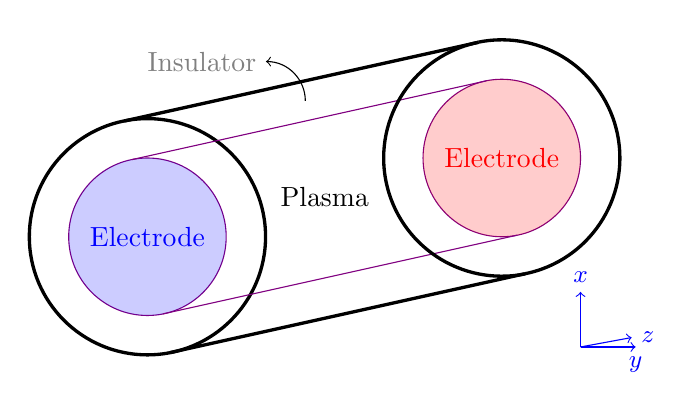
\begin{tikzpicture}
    \coordinate (O1) at (0,0);
    \draw[violet] (O1) circle (1) node[blue] {Electrode};
    \fill[blue, opacity=0.2] (O1) circle (1);
    \draw[very thick] (O1) circle (1.5);
    \coordinate (O2) at (4.5,1);
    \draw[violet] (O2) circle (1);
    \node at (O2) {\textcolor{red}{Electrode}};
    \node at (barycentric cs:O1=1,O2=1) {Plasma}; 
    \fill[red, opacity=0.2] (O2) circle (1);
    \coordinate (S1) at ([shift={(-0.196,0.98)}]O1);
    \coordinate (S2) at ([shift={(-0.196,0.98)}]O2);
    \coordinate (P1) at ([shift={(0.196,-0.98)}]O1);
    \coordinate (P2) at ([shift={(0.196,-0.98)}]O2);
    \draw[violet] (S1) -- (S2);
    \draw[violet] (P1) -- (P2);
    \coordinate (SS1) at ([shift={({-0.196*1.5},{0.98*1.5})}]O1);
    \coordinate (SS2) at ([shift={({-0.196*1.5},{0.98*1.5})}]O2);
    \coordinate (PP1) at ([shift={({0.196*1.5},{-0.98*1.5})}]O1);
    \coordinate (PP2) at ([shift={({0.196*1.5},{-0.98*1.5})}]O2);
    \draw[very thick] (SS1) -- (SS2);
    \draw[very thick] (PP1) -- (PP2); 
    \draw[black, very thick] (SS2) arc (101.31:180+101.31:1.5);
    \draw[very thick] (PP2) arc (101.31-180:101.31:1.5);
    \draw[-to] (barycentric cs:SS1=1,SS2=1,S1=1,S2=1) to[out=90,in=0] ([shift={(-0.5,0.5)}]barycentric cs:SS1=1,SS2=1,S1=1,S2=1) node[left, gray] {Insulator};
    \begin{scope}[shift={(5.5,-1.4)}]
    \draw[blue, -to] (0,0) -- (0.65,0.12) node[right]{\small $z$};
    \draw[blue, -to] (0,0) -- (0,0.7) node[above]{\small $x$};
    \draw[blue, -to] (0,0) -- (0.7,0) node[below]{\small $y$};
    \end{scope}
    \end{tikzpicture}}
\end{minipage}
\begin{minipage}{0.49\textwidth}
    \resizebox{1.1\textwidth}{!}{ 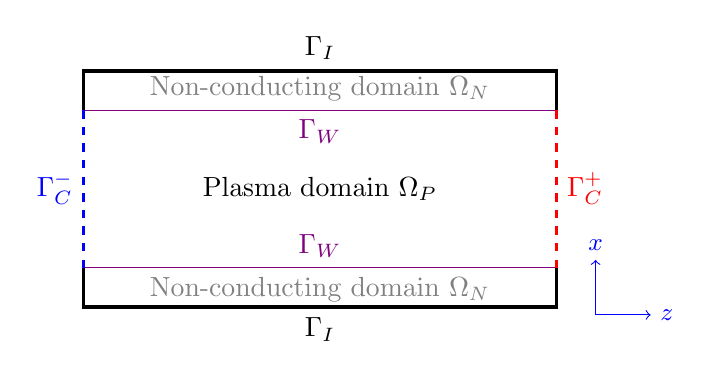
\begin{tikzpicture}
        \coordinate (A1) at (0,1.5);
        \coordinate (A2) at (0,1);
        \coordinate (A3) at (0,-1);
        \coordinate (A4) at (0,-1.5);
        \coordinate (B1) at (6,1.5);
        \coordinate (B2) at (6,1);
        \coordinate (B3) at (6,-1);
        \coordinate (B4) at (6,-1.5);
        \draw[violet] (A2) -- node[above]{\color{gray}Non-conducting domain $\Omega_N$} node[black, below]{\textcolor{violet}{$\Gamma_W$}} (B2);
        \draw[violet] (A3) -- node[below]{\color{gray}Non-conducting domain $\Omega_N$} node[black, above]{\textcolor{violet}{$\Gamma_W$}} (B3);
        \draw[very thick] (A2) -- (A1) -- node[above]{$\Gamma_I$}  (B1) -- (B2);
        \draw[very thick] (A3) -- (A4) -- node[below]{$\Gamma_I$} (B4) -- (B3);
        \draw[very thick, dashed, blue] (A2) -- node[left] {$\Gamma_C^-$} (A3);
        \draw[very thick, dashed, red]  (B2) -- node[right] {$\Gamma_C^+$}  (B3);
        \node at (3,0) {Plasma domain $\Omega_P$};
        \begin{scope}[shift={(6.5,-1.6)}]
        \draw[blue, -to] (0,0) -- (0,0.7) node[above]{\small $x$};
        \draw[blue, -to] (0,0) -- (0.7,0) node[right]{\small $z$};
        \end{scope}
    \end{tikzpicture}}
\end{minipage}
\caption{The right figure shows the cross section in the $x$-$z$ plane and the different
  parts of the boundary and interfaces.}
\label{fig:domain_sketch}
\end{figure}
We summarize the boundary conditions for both sets of equations:

\begin{minipage}[t]{0.49\textwidth}
    \textbf{For the Euler equations:}
    \begin{align*}
    \mathbf{u_*}\cdot \mathbf{n} &= 0 \ \ \text{on} \ \ \Gamma_W, \\
    \nabla \mathbf{u_*} \cdot \mathbf{n} &= \mathbf{0} \ \ \text{on} \ \ \Gamma_C, \\
    \nabla n_* \cdot \mathbf{n} &= 0 \ \ \text{on} \ \ \Gamma_W \cup \Gamma_C, \\
    \nabla e_* \cdot \mathbf{n} &= 0 \ \ \text{on} \ \ \Gamma_W \cup \Gamma_C.
\end{align*}
\end{minipage}
\begin{minipage}[t]{0.49\textwidth}
    \textbf{For Maxwell's equations:}
    \begin{align*}
    \mathbf{D} \cdot \mathbf{n} = 0\ \ &\text{on} \ \  \partial\Omega,  \\
    \mathbf{B} \cdot \mathbf{n} = 0\ \ &\text{on} \ \  \Gamma_I,  \\
    \varphi = \varphi^\pm(t)\ \ &\text{on} \ \ \Gamma_C^\pm.
    \end{align*}
\end{minipage}

\vspace{10pt}
\begin{remark}
    No interface condition for Maxwell's equations is needed on $\Gamma_W$.
\end{remark}

\begin{remark} For a geometric setting with non-trivial topology, e.g. with a tunnel,
  $\nabla \times \mathbf{E}\cdot\mathbf{n} = 0$ does guarantee the existence of a surface
  potential $\varphi$ satisfying $\mathbf{E}_t = \nabla_\Gamma\varphi$. One needs to
  include co-homology vector fields \cite{Hiptmair_2021}.
\end{remark}

\subsection{Stabilization in $\Omega_{N}$}
\label{sec:reform_continuous}

No plasma fills the non-conducting domain $\Omega_N$ (see Fig. \ref{fig:domain_sketch}),
and, consequently, the Maxwell system in $\Omega_N$ reduces to 
\begin{subequations}
  \label{eq:mxon}
\begin{align}
    \partial_t \mathbf{B} + \nabla \times \mathbf{E} &= 0, \label{equ:faraday_ins}\\ 
    \lambda^2 \partial_t \mathbf{D} - \nabla \times \mathbf{H} &= 0,  \label{equ:ampere_ins}\\
    \nabla \cdot \mathbf{B} &= 0, \label{equ:gauss_B_ins}\\
    \lambda^2 \nabla \cdot \mathbf{D} &= 0 \label{equ:gauss_D_ins}.
\end{align}
\end{subequations}
In a non-neutral regime where $\lambda = \mathcal{O}(1)$, the Maxwell system in $\Omega_N$
is well-posed and Gauss's laws (\ref{equ:gauss_B_ins}) (\ref{equ:gauss_D_ins}) are
redundant as long as they are satisfied at initial time. Nonetheless, as the system
approaches the quasi-neutral limit as $\lambda \rightarrow 0$, Gauss's law for the
$\mathbf{D}$-field (\ref{equ:gauss_D_ins}) becomes degenerate. Schemes based on this set
of PDEs would become unstable as $\lambda \rightarrow 0$. The vanishing divergence
constraint would evaporate as $\nabla \cdot \mathbf{D} = 0/\lambda^2 = 0$ would not hold
numerically when $\lambda^2$ becomes extremely small.

To view this issue from another perspective, we examine the limit Maxwell system in
$\Omega_N$:
\begin{subequations}
\begin{align}
    \partial_t \mathbf{B} + \nabla \times \mathbf{E} &= 0, \label{equ:faraday_ins_limit}\\ 
    - \nabla \times \mathbf{H} &= 0,  \label{equ:ampere_ins_limit}\\
    \nabla \cdot \mathbf{B} &= 0, \label{equ:gauss_B_ins_limit}\\
    \nabla \cdot \mathbf{D} &= 0 \label{equ:gaus_D_ins_limit}.
\end{align}
\end{subequations}

Again, Gauss's law for the $\mathbf{B}$-field (\ref{equ:gauss_B_ins_limit}) is redundant,
while Gauss's law for the $\mathbf{D}$-field (\ref{equ:gaus_D_ins_limit}) is no longer a
consequence of Amp\`{e}re's law (\ref{equ:ampere_ins_limit}). However,
\eqref{equ:gaus_D_ins_limit} is essential for the well-posedness of the problem \cite[][p.
7]{ana_2010}. Obviously, the degeneracy of Gauss's law for the $\mathbf{D}$-field in the
system (\ref{equ:faraday_ins_limit}) to (\ref{equ:gaus_D_ins_limit}) as
$\lambda \rightarrow 0$ poses some problem. In other words, the set of equations
(\ref{equ:faraday_ins_limit}) to (\ref{equ:gaus_D_ins_limit}) switches to an ill-posed
situation for $\lambda=0$. I computations this will manifest itself as instability 
already for ${\lambda>0}$.

As a remedy, we propose the following reformulation which introduces a scalar Lagrange
multiplier $\psi$ and removes the $\lambda^2$ prefactor in Gauss's law for the
$\mathbf{D}$-field:
\begin{subequations}
\begin{align}
    \partial_t \mathbf{B} + \nabla \times \mathbf{E} &= 0, \label{equ:faraday_ins_reform}\\ 
    \lambda^2 \partial_t \mathbf{D} - \nabla \times \mathbf{H} + \colorbox{orange!20}{$\nabla \psi$} &= 0,  \label{equ:ampere_ins_reform}\\
    \nabla \cdot \mathbf{B} &= 0, \label{equ:gauss_B_ins_reform}\\
    \nabla \cdot \mathbf{D} &= 0 \label{equ:gauss_D_ins_reform}.
\end{align}
\end{subequations}

Supplemented with the boundary condition $\psi = 0$ on $\partial\Omega_N$, one can check
that (\ref{equ:faraday_ins_reform}) to (\ref{equ:gauss_D_ins_reform}) are equivalent to
the original formulation (\ref{equ:faraday_ins})-(\ref{equ:gauss_D_ins}) by verifying that
$\psi = 0$ in $\Omega_N$. This is done by taking the divergence of
(\ref{equ:ampere_ins_reform}), which results in $\Delta\psi = 0$ and the zero Dirichlet
boundary condition gives vanishing $\psi$. The importance of this reformulation will
become clear through numerical experiments, see Section \ref{sec:numerical_experiment}.

We point out that this reformulation is not needed in the plasma domain $\Omega_P$ since
the Maxwell system is uniformly well-posed for $\lambda \in [0,1]$ thanks to the existence
of an electric current and its dependence on the $\mathbf{E}$-field.

\begin{comment}
  To devise an AP scheme, the dependence of the stability constraints of $h$ on $\lambda$
  has to be removed. This is mainly achieved by utilizing implicit time-stepping for
  certain terms. As is summarized by \cite{degond_2017}, AP schemes aim to bridge several
  sets of equations describing the system in different regimes, rather than to alleviate
  the stability constraints of the numerical methods. In this sense, a fully-implicit
  scheme is likely to be overkill and thus a smart construction is necessary. The second
  consideration goes to the identification of a compatible boundary conditions for both
  regimes, which would be shown to be essential for the numerical stability.

  In the following sections, we first briefly discuss the 1D scheme for the Maxwell-Euler
  system devised by \cite{degond_2012} on which our work us built. This section also
  serves as a preliminary case study such that readers can better understand the 3D
  scheme.
\end{comment}

\section{Spatial Discretization} \label{sec:spatial_discretization}
\subsection{Primal-dual Staggered Meshes} \label{sec:mesh-duality}
\subsubsection{Definition and Geometric Construction}

To prepare the spatial discretization of the Maxwell-Euler system, we introduce
primal-dual staggered meshes, a key component of the discrete exterior calculus (DEC)
discretization of Maxwell's equations. The spatial domain is covered by two meshes
interlacing with each other, denoted by a mesh doublet
$(\mathcal{M}, \Tilde{\mathcal{M}})$ for primal mesh and dual mesh respectively. The
fundamental duality property requires that \emph{each edge of one mesh penetrates a face
  of the other mesh and that each vertex of one mesh lies inside of a cell of the other
  mesh} \cite[][Sec. 2]{weiland_2003}. Examples are shown in Fig.~\ref{fig:cartesian}.

To clarify the notation, in three dimensions the primal mesh $\mathcal{M}$ is a cell
complex defined by the set of mesh entities $\{P, L, A, V\}$\footnote{The notation here is
  a bit sloppy. $P, L, A, V$ can refer to a single entity or a set of entities depending
  on the context.} denoting \emph{vertices (points), edges, faces} and \emph{cells}
respectively. In the same way, the dual mesh $\Tilde{\mathcal{M}}$ is defined by
$\{\Tilde{P}, \Tilde{L}, \Tilde{A}, \Tilde{V}\}$. The entities of two meshes are
connected by one-on-one pairings $P \leftrightarrow \Tilde{V}$,
$L \leftrightarrow \Tilde{A}$, $A \leftrightarrow \Tilde{L}$ and
$V \leftrightarrow \Tilde{P}$, which arise in a very natural way:
$P(\Tilde{P} \text{ resp.,})$ corresponds to $\Tilde{V}(V \text{ resp.,})$ in which it
lies and $L(\Tilde{L} \text{ resp.,})$ penetrates a corresponding
$\Tilde{A}(A \text{ resp.,})$. According to their dimensions, vertices, edges, faces and
cells are also called 0-dim, 1-dim, 2-dim and 3-dim entities respectively. Moreover, we
denote by $N_\ast, \ast \in \{P, \Tilde{P}, L, \Tilde{L},A, \Tilde{A},V, \Tilde{V}\}$ the
total number of entities in $\mathcal{M}, \Tilde{\mathcal{M}}$.

In 2D we construct the pair of meshes based on the Delaunay-Voronoi approach: we start with a
Delaunay triangulation $\mathcal{M}$ of the domain and construct $\Tilde{\mathcal{M}}$ by
connecting \emph{circumcenters} of any two adjacent triangles, see Fig. \ref{fig:2d-mesh}.
In three dimensions, the meshes are constructed by extruding the 2D meshes vertically
along one axis in a staggered manner \cite[][Sec. 3.1]{Marrone_2001}. See an example in
Fig. \ref{fig:2d-extrusion}. In this way, the meshes are composed of prisms. This
particular choice is compatible with the cylindrical geometric setting that we are in, see
Fig. \ref{fig:domain_sketch}. For a general setting, one can directly decompose the domain
into tetrahedrons and constructs the Voronoi grid, but the procedure is more
complicated. The meshes for the cylindrical domain are displayed in
Fig. \ref{fig:primal_dual_meshes}.

The geometric orthogonality between $L \leftrightarrow \Tilde{A}$ and
$A \leftrightarrow \Tilde{L}$ is satisfied and will be a crucial property for
approximating the material laws on the discrete level (which is the so-called discrete
Hodge operator \cite{hip_1999, bossavit1999}), as will be shown in Section \ref{sec:fit}.

\begin{remark}
  The use of the Delaunay-Voronoi based primal-dual meshes is problematic when there are
  triangles with an obtuse angle in $\mathcal{M}$. In this case their circumcenters lie
  outside the triangles and the intersection between edges and faces is violated. An
  alternative approach is barycenter-based dual meshes, which are not restricted to an
  acute-angle triangulation \cite[][Sec. 4.2]{Marrone_2001}.
\end{remark}



\begin{figure}
    \begin{subfigure}[b]{0.35\textwidth}
    \centering
    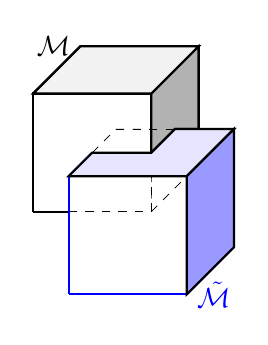
\begin{tikzpicture}[scale = 0.3]
            \def\style{thick}
            \draw[\style] (0,0) -- (1.5,0);
            \draw[\style] (0,0) -- (0,5) -- (5,5) -- (5,2.5);
            \draw[\style] (0,5) -- (2,7) node[left]{$\mathcal{M}$} -- (7,7) -- (5,5);
            \draw[\style] (7,7) -- (7,3.5);
            \draw[dashed, very thin] (1.5, 0) -- (5,0);
            \draw[dashed, very thin] (5,0) -- (5,2.5);
            \draw[dashed, very thin] (5,0) -- (7,2);
            \draw[dashed, very thin] (7,2) -- (7,3.5);
            
            \draw[fill = gray!60,\style] (5,2.5) -- (6,3.5) -- (7,3.5) -- (7,7) -- (5,5) -- cycle;
            \draw[fill = gray!10,\style] (0,5) -- (5,5) -- (7,7) -- (2,7) -- cycle;
            \draw[dashed, very thin] (5,0) -- (6.5,1.5) -- (5,1.5) -- cycle;
            
            \begin{scope}[shift={(1.5,-3.5)}]
            \draw[blue,\style] (0,0) -- (5,0)  node[right]{$\Tilde{\mathcal{M}}$};
            \draw[blue,\style] (5,0) -- (5,5);
            \draw[blue,\style] (5,5) -- (0,5);
            \draw[blue,\style] (0,5) -- (0,0);
            \draw[blue,\style] (0,5) -- (1,6);
            \draw[blue,\style] (4.5,7) -- (7,7);
            \draw[blue,\style] (7,7) -- (5,5);
            \draw[blue,\style] (7,7) -- (7,2);
            \draw[blue,\style] (7,2) -- (5,0);
            \draw[dashed, very thin] (1,6) -- (2,7);
            \draw[dashed, very thin] (2,7) -- (4.5,7);
            \draw[fill = blue!10,\style] (0,5) -- (5,5) -- (7,7) -- (4.5,7) -- (3.5, 6) -- (1,6) -- cycle;
            \draw[fill = blue!40,\style] (5,0) -- (7,2) -- (7,7) -- (5,5) -- cycle;
            \draw[dashed, very thin] (1,6) -- (2,7) -- (3.5,7) -- (3.5,6) -- cycle;
            \end{scope}
        \end{tikzpicture}
        \caption{3D case (Cartesian)}
        \label{fig:cartesian}
    \end{subfigure}
    \begin{subfigure}[b]{0.3\textwidth}
    \centering
    \resizebox{0.6\textwidth}{!}{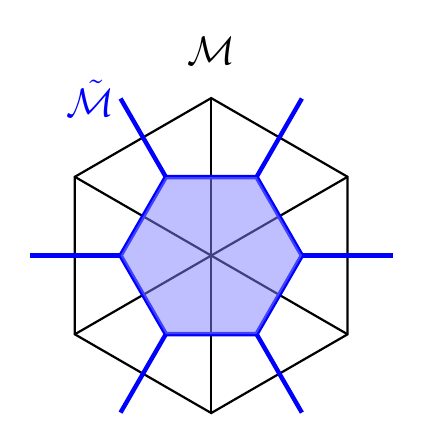
\begin{tikzpicture}[scale = 1]
    \def\primalstyle{thick}
    \def\dualstyle{ultra thick}
    \coordinate (P0) at (0cm, 0cm);
    \foreach \i in {1,2,...,6}
    {
    \coordinate (P\i) at ({60*\i-30}:2cm);
    \draw[\primalstyle] (P0) -- (P\i);
    }
    \draw[\primalstyle] (P1) -- (P2) node[above=3mm]{\Large $\mathcal{M}$} node[left=11mm]{\Large \color{blue} $\Tilde{\mathcal{M}}$} -- (P3) -- (P4) -- (P5) -- (P6) -- cycle;
    \foreach \i in {1,2,...,6}
    {
    \coordinate (D\i) at ({60*\i-60}:{2./1.737});
    \coordinate (DD\i) at ({60*\i-60}:{4./1.737});
    }
    \draw[blue,\dualstyle] (D1) -- (D2) -- (D3) -- (D4) -- (D5) -- (D6) -- cycle;
    \foreach \i in {1,2,...,6}
    {
    \draw[blue,\dualstyle] (D\i) -- (DD\i);
    }
    \fill[blue!50, opacity=0.5] (D1) -- (D2) -- (D3) -- (D4) -- (D5) -- (D6) -- cycle;
    \end{tikzpicture}}
    \caption{2D case}
    \label{fig:2d-mesh}
    \end{subfigure}
    \begin{subfigure}[b]{0.35\textwidth}
    \centering
    \resizebox{0.9\textwidth}{!}{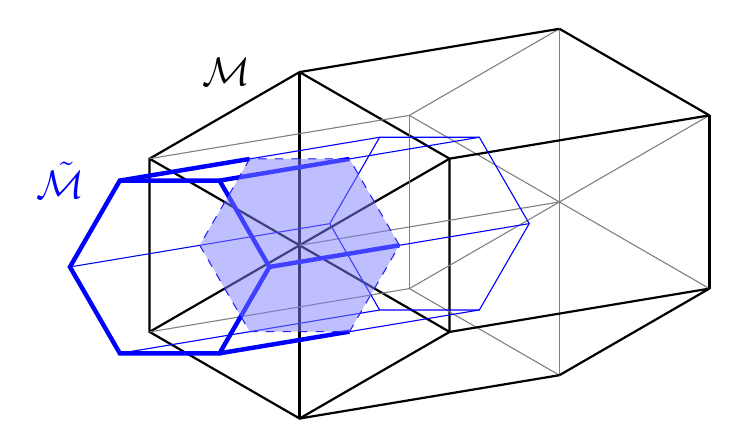
\begin{tikzpicture}[scale=1.1]
    \def\primalstyle{thick}
    \def\dualstyle{thick}
    \coordinate (P0) at (0cm, 0cm);
    \foreach \i in {1,2,...,6}
    {
    \coordinate (P\i) at ({60*\i-30}:2cm);
    \draw[\primalstyle] (P0) -- (P\i);
    }
    \draw[\primalstyle] (P1) -- (P2) node[left=5mm]{\Large $\mathcal{M}$} -- (P3) -- (P4) -- (P5) -- (P6) -- cycle;
    \begin{scope}[shift={(3cm,0.5cm)}]
        \coordinate (PP0) at (0cm, 0cm);
        \foreach \i in {1,2,...,6}
        {
        \coordinate (PP\i) at ({60*\i-30}:2cm);
        \draw[gray] (PP0) -- (PP\i);
        }
    \end{scope}
    
    \draw[\primalstyle] (PP1) -- (PP2);
    \draw[gray] (PP2) -- (PP3);
    \draw[gray] (PP3) -- (PP4);
    \draw[gray] (PP4) -- (PP5);
    \draw[\primalstyle] (PP5) -- (PP6);
    \draw[\primalstyle] (PP6) -- (PP1);
    
    \draw[gray] (P0) -- (PP0);
    \draw[\primalstyle] (P1) -- (PP1);
    \draw[\primalstyle] (P2) -- (PP2);
    \draw[gray] (P3) -- (PP3);
    \draw[gray] (P4) -- (PP4);
    \draw[\primalstyle] (P5) -- (PP5);
    \draw[\primalstyle] (P6) -- (PP6);
    
    \foreach \i in {1,2,...,6}
    {
    \coordinate (D\i) at ({60*\i-60}:{2./1.737});
    }
    \draw[dashed, blue] (D1) -- (D2) -- (D3) -- (D4) -- (D5) -- (D6) -- cycle;
    \begin{scope}[shift={(1.5,0.25)}]
        \foreach \i in {1,2,...,6}
        {
        \coordinate (DD\i) at ({60*\i-60}:{2./1.737});
        }
    \end{scope}
    \draw[blue] (DD1) -- (DD2) -- (DD3) -- (DD4) -- (DD5) -- (DD6) -- cycle;
    \draw[blue] (D1) -- (DD1);
    \draw[blue] (D2) -- (DD2);
    \draw[blue] (D3) -- (DD3);
    \draw[blue] (D4) -- (DD4);
    \draw[blue] (D5) -- (DD5);
    \draw[blue] (D6) -- (DD6);
    
    \begin{scope}[shift={(-1.5,-0.25)}]
        \foreach \i in {1,2,...,6}
        {
        \coordinate (DDD\i) at ({60*\i-60}:{2./1.737});
        }
    \end{scope}
    \draw[blue, ultra thick] (DDD1) -- (DDD2) -- (DDD3) node[left=3mm]{\textcolor{blue}{\Large $\Tilde{\mathcal{M}}$}} -- (DDD4) -- (DDD5) -- (DDD6) -- cycle;
    \draw[blue, ultra thick] (D1) -- (DDD1);
    \draw[blue, ultra thick] (D2) -- (DDD2);
    \draw[blue, ultra thick] (D3) -- (DDD3);
    \draw[blue] (D4) -- (DDD4);
    \draw[blue] (D5) -- (DDD5);
    \draw[blue, ultra thick] (D6) -- (DDD6);
    \fill[blue!50, opacity=0.5] (D1) -- (D2) -- (D3) -- (D4) -- (D5) -- (D6);
    \end{tikzpicture}}
    \caption{3D case (2D extrusion)}
    \label{fig:2d-extrusion}
    \end{subfigure}
    \hfill
    \caption{Illustration of primal and dual meshes. \textbf{(a)} A Cartesian case
      (``staggered grids'') \textbf{(a)} A Delaunay-Voronoi grid in 2D \textbf{(c)} The
      extrusion of 2D mesh: six triangular prisms are primal cells (with black and
      gray edges). One dual cell, which is a hexagonal prism, is depicted by blue edges. The
      dashed hexagon represents the intersection of the dual cell and primal cells. }
    \label{fig:illustration_primal_dual}
\end{figure}

\subsubsection{Orientation and Incidence Matrices}

Each geometric entity in the primal mesh $\mathcal{M}$ is (arbitrarily) endowed with an
\emph{internal orientation}\footnote{This notion should not be confused with \emph{inner
    orientation}, which has a slightly different definition, see
  \cite[][Sec. 3.1]{tonti_2002}.}. The notion is illustrated in
Fig. \ref{fig:orientation}. For the entities of the dual mesh $\Tilde{\mathcal{M}}$, we
set their internal orientations to be aligned with their corresponding primal entities
according to the bijective pairings, i.e. edges penetrate faces.

Another orientation attribute, \emph{induced orientation}, is defined as follows: an induced orientation of a k-dim entity $f$ with respect to a (k+1)-dim entity $f'$, satisfying $f \subset \partial f' $, is determined by the internal orientation of $f'$ according to the rules shown in Fig. \ref{fig:orientation}. 

This information can be described by matrices with entries in $\{0,-1,+1\}$, called \emph{incidence matrices}. To describe the primal face-to-edge relation, for instance, a sparse matrix $\mathbb{C} \in \mathbb{R}^{N_A \times N_L}$ is assembled whose $(i,j)$-entry is assigned $+1$ if the internal orientation of edge $L_j$ and its induced orientation with respect to face $A_i$ coincides; it is assigned $-1$ if two orientations are opposite; and assigned $0$ if $L_j$ is not a subset of the boundary of $A_i$. We will see later that $\mathbb{C}$ functions as a discrete version of the rotation operator. The other incidence matrices are constructed in the same manner, see Tab. \ref{tab:incidence_mat} for a summary. Given the relationship of orientations of $\mathcal{M}$ and $\Tilde{\mathcal{M}}$, we can derive the relations listed in Tab. \ref{tab:incidence_relation}.  

\begin{table}[h!]
    \centering
    \begin{tabular}{c c l l}
    \hline
         Matrix & Size & Incidence relation & Intuition  \\
    \hline
         $\mathbb{D}\ (\Tilde{\mathbb{D}})$ & $N_V \times N_A\ (N_{\Tilde{V}} \times N_{\Tilde{A}})$ & cell $\rightarrow$ face & discrete divergence \\
         $\mathbb{C}\ (\Tilde{\mathbb{C}})$ & $N_A \times N_L\ (N_{\Tilde{A}} \times N_{\Tilde{L}})$ & face $\rightarrow$ edge & discrete rotation \\
         $\mathbb{G}\ (\Tilde{\mathbb{G}})$ & $N_L \times N_P\ (N_{\Tilde{L}} \times N_{\Tilde{P}})$ & edge $\rightarrow$ vertex & discrete gradient
         \\
    \hline
    \end{tabular}
    \caption{Summary of incidence matrices}
    \label{tab:incidence_mat}
\end{table}

\begin{table}[h!]
    \centering
    \begin{tabular}{c c}
    \hline
         Property of incidence matrices & Corresponding rule in vector analysis \\
    \hline
         $\mathbb{G}^T = -\Tilde{\mathbb{D}}$  &  $\nabla ^* = - (\nabla \cdot) $\\
         $\mathbb{C}^T = \Tilde{\mathbb{C}}$   &  $(\nabla \times) ^* = (\nabla \times) $\\
         $\mathbb{D}^T = -\Tilde{\mathbb{G}}$  &  $(\nabla \cdot) ^* = - \nabla $\\
         $\mathbb{C}\mathbb{G} = \mathbf{0}, \Tilde{\mathbb{C}}\Tilde{\mathbb{G}} = \mathbf{0}$  &  $(\nabla \times)\circ \nabla = 0$ \\
         $\mathbb{D}\mathbb{C} = \mathbf{0}, \Tilde{\mathbb{D}}\Tilde{\mathbb{C}} = \mathbf{0}$   &  $(\nabla \cdot) \circ ( \nabla \times) = 0$ \\
    \hline
        \small $\ast$ denotes adjoint operator.
    \end{tabular}
    \caption{Relations between incidence matrices}
    \label{tab:incidence_relation}
\end{table}

These matrices are topological and thus invariant under smooth deformation of the domain. In the next section, we will show that they play a crucial role in constructing discrete Maxwell's equations. 

\begin{figure}
    \centering
    \begin{minipage}{0.2\textwidth}
    \centering
    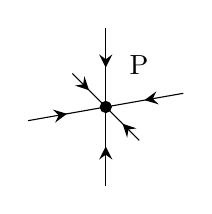
\begin{tikzpicture}
        \coordinate (P0) at (0,0);
        \coordinate (P1) at (10:1); 
        \coordinate (P2) at (90:1);
        \coordinate (P3) at (190:1);
        \coordinate (P4) at (270:1);
        \coordinate (P5) at (135:0.6);
        \coordinate (P6) at (-45:0.6);
        \foreach \i in {1,2,...,6} 
        {
            \draw[decoration={markings, mark= at position 0.5 with {\arrow[scale=1.5]{stealth}}},postaction={decorate}] (P\i) -- (P0);
        }
        \draw[fill=black] (P0) circle (0.07) node[yshift=15pt, xshift=12pt]{P}; 
    \end{tikzpicture}
    \end{minipage}
    \begin{minipage}{0.2\textwidth}
    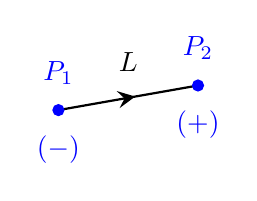
\begin{tikzpicture}
        \coordinate (P1) at (0,0);
        \coordinate (P2) at (10:1.8);
        \draw[decoration={markings, mark= at position 0.55 with {\arrow[scale=1.5]{stealth}}},postaction={decorate}, thick] (P1) -- node[above=2mm]{$L$} (P2);
        \draw[blue, fill=blue] (P1) circle (0.07) node[above=2mm] {\color{blue}$P_1$} node[below=2mm] {\color{blue}$(-)$};
        \draw[blue, fill=blue] (P2) circle (0.07) node[above=2mm] {\color{blue}$P_2$} node[below=2mm] {\color{blue}$(+)$};
    \end{tikzpicture}
    \end{minipage}
    \begin{minipage}{0.2\textwidth}
    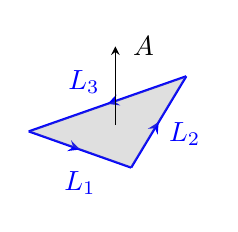
\begin{tikzpicture}
        \coordinate (Q1) at (0,0);
        \coordinate (Q2) at (1.3cm, -0.46cm);
        \coordinate (Q3) at (2.0cm, 0.7cm);
        \draw[decoration={markings, mark= at position 0.5 with {\arrow[scale=1]{stealth}}}, postaction={decorate}, thick, blue] (Q1) -- node[below=1.5mm]{$L_1$} (Q2);
        \draw[decoration={markings, mark= at position 0.5 with {\arrow[scale=1]{stealth}}}, postaction={decorate},  thick, blue] (Q2) -- node[right,yshift=-1.5mm]{$L_2$} (Q3);
        \draw[decoration={markings, mark= at position 0.5 with {\arrow[scale=1]{stealth}}}, postaction={decorate},  thick, blue] (Q3) -- node[above,xshift=-3mm] {$L_3$}(Q1);
        \fill[black!50, opacity=0.25] (Q1) -- (Q2) -- (Q3);
        \draw[-stealth](barycentric cs:Q1=1,Q2=1,Q3=1) -- ([shift={(0,1cm)}] barycentric cs:Q1=1,Q2=1,Q3=1) node[right,xshift=1mm] {$A$}; 
    \end{tikzpicture}
    \end{minipage}
    \begin{minipage}{0.2\textwidth}
    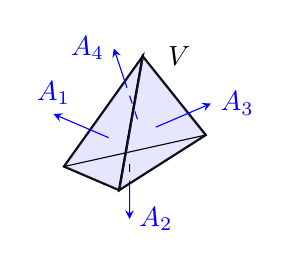
\begin{tikzpicture}
        \coordinate (S1) at (0,0);
        \coordinate (S2) at (-0.7,0.3);
        \coordinate (S3) at (1.1,0.7);
        \coordinate (S4) at (0.3,1.7);
        \draw[thick] (S1) -- (S2) -- (S4) -- cycle;
        \fill[blue!50, opacity=0.2] (S1) -- (S2) -- (S4);
        \draw[thick] (S1) -- (S3) -- (S4) -- cycle;
        \fill[blue!50, opacity=0.2] (S1) -- (S3) -- (S4);
        \draw[thin] (S2) -- (S3);
        \draw[-stealth, blue] (barycentric cs:S1=1,S2=1,S4=1) -- ([shift={(-0.7,0.3)}] barycentric cs:S1=1,S2=1,S4=1) node[above] {$A_1$};
        \coordinate (O1) at (barycentric cs:S1=1,S2=1,S3=1);
        \coordinate (O2) at ([shift={(0,-0.7)}] barycentric cs:S1=1,S2=1,S3=1);
        \coordinate (S)  at (intersection of O1--O2 and S1--S3);
        \draw[dashed] (O1) -- (S);
        \draw[-stealth, blue] (S) -- (O2) node[right] {$A_2$};
        \draw[-stealth, blue] (barycentric cs:S1=1,S3=1,S4=1) -- ([shift={(0.7,0.3)}] barycentric cs:S1=1,S3=1,S4=1) node[right] {$A_3$} ;
        \coordinate (OO1) at (barycentric cs:S2=1,S3=1,S4=1);
        \coordinate (OO2) at ([shift={(-0.3,0.9)}] barycentric cs:S2=1,S3=1,S4=1);
        \coordinate (SS)  at (intersection of OO1--OO2 and S2--S4);
        \draw[dashed, blue] (OO1) -- (SS);
        \draw[-stealth, blue] (SS) -- (OO2) node[left] {$A_4$};
        \node at (S4) [right, xshift=2mm] {$V$};
    \end{tikzpicture}
    \end{minipage}
    \caption{Illustration of internal and induced orientations. The internal orientation of each entity is depicted in black: vertices are oriented as \emph{sink} by default; edges are oriented by their pointing direction; faces are oriented by their normal vector; cells are oriented positive by default. The induced orientations are depicted in blue: the ending vertex of an edge is negatively oriented while the starting point is positively oriented; the orientations of edges with respect to a face obey the right-hand rule; a face of a cell are oriented by its outer normal vector. }
    \label{fig:orientation}
\end{figure}

\subsubsection{Cut-off Boundary}

The primal mesh $\mathcal{M}$ is generated first and resolves the domain boundary
$\partial\Omega$. The dual mesh $\Tilde{\mathcal{M}}$ is generated afterwards. To make
both meshes aligned at the boundary, we have to truncate the \emph{dual} entities near the
boundary. In addition, auxiliary geometric entities are needed to close
$\Tilde{\mathcal{M}}$, see Fig.~\ref{fig:illustraion_dual_boundary}.

Note that the auxiliary edges might not be straight and the auxiliary faces might not be
flat as is shown in Fig. \ref{fig:illustraion_dual_boundary}, which necessitates a
versatile data structure to include such situations. In the following, the auxiliary
entities would be treated as dual entities, which limits the validity of the relations in
Tab. \ref{tab:incidence_relation} to interior part of $\Tilde{\mathcal{M}}$. For a more
systematic illustration that considers the boundary dual entities, see
\cite[][Sec. 5]{hip_1999}.

\begin{figure}
    \centering
    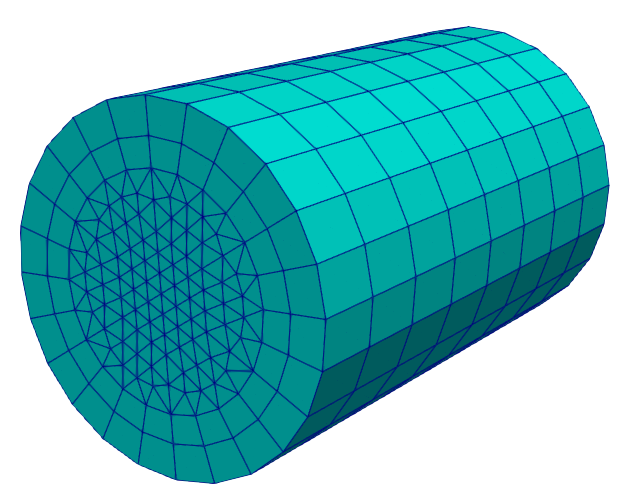
\includegraphics[scale=0.3]{primal_mesh.png}
    \hspace{1cm}
    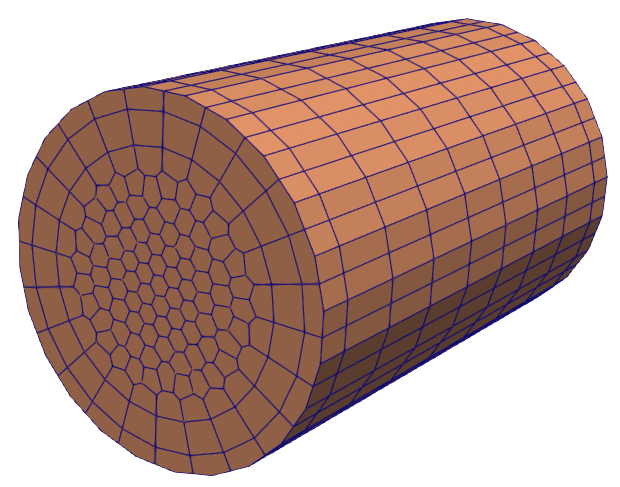
\includegraphics[scale=0.3]{dual_mesh.png}
    \caption{Primal mesh (left) and dual mesh (right).}
    \label{fig:primal_dual_meshes}
\end{figure}

\begin{figure}
    \begin{subfigure}[b]{0.3\textwidth}
        \centering
        \begin{tikzpicture}
            \colorlet{dual}{blue}
            \tkzDefPoint(0,0){P1} 
            \tkzDefPoint(1,1){P1}
            \tkzDefPoint(1.1,-0.8){P2} 
            \tkzDefPoint(0.4,-1.4){P3} 
            \tkzDefPoint(2,0.9){P4} 
            \tkzDefPoint(1.4, 0){P5}
            \tkzDefPoint(2.3, 0){P6}
            \tkzDefPoint(2.1,-1){P7} 
            \tkzDefPoint(1.6,-1.7){P8} 
            \foreach \i in {0,...,8} {\tkzDrawPoints(P\i)}
            %\foreach \i in {0,...,8} {\tkzLabelPoints(P\i)}
            \tkzDrawSegments(P1,P0 P1,P4 P1,P5 P5,P0 P5,P4 P5,P2 P5,P6 P4,P6 P0,P2 P2,P7 P5,P7 P6,P7 P3,P0 P3,P2 P3,P8 P2,P8 P8,P7)
            \tkzDefTriangleCenter[circum](P1,P0,P5) \tkzGetPoint{O1} 
            \tkzDefTriangleCenter[circum](P1,P4,P5) \tkzGetPoint{O2}
            \tkzDefTriangleCenter[circum](P4,P6,P5) \tkzGetPoint{O3}
            \tkzDefTriangleCenter[circum](P2,P0,P5) \tkzGetPoint{O4} 
            \tkzDefTriangleCenter[circum](P2,P7,P5) \tkzGetPoint{O5}
            \tkzDefTriangleCenter[circum](P2,P0,P3) \tkzGetPoint{O6}
            \tkzDefTriangleCenter[circum](P2,P3,P8) \tkzGetPoint{O7}
            \tkzDefTriangleCenter[circum](P2,P7,P8) \tkzGetPoint{O8}
            \tkzDefTriangleCenter[circum](P5,P6,P7) \tkzGetPoint{O9}
            \foreach \i in {1,...,9} {\tkzDrawPoints[dual](O\i)}
            %\foreach \i in {1,...,9} {\tkzLabelPoints(O\i)}
            \tkzDrawSegments[dual](O1,O2 O2,O3 O3,O9 O9,O5 O5,O4 O1,O4 O4,O6 O6,O7 O7,O8 O8,O5 O5,O9)
            \tkzDefMidPoint(P0,P1) \tkzGetPoint{M0} \tkzDrawSegment[dual, add= 0 and 1](O1, M0)
            \tkzDefMidPoint(P1,P4) \tkzGetPoint{M1} \tkzDrawSegment[dual, add= 0 and 1](O2, M1)
            \tkzDefMidPoint(P4,P6) \tkzGetPoint{M2} \tkzDrawSegment[dual, add= 0 and 1](O3, M2)
            \tkzDefMidPoint(P6,P7) \tkzGetPoint{M3} \tkzDrawSegment[dual, add= 0 and 1](O9, M3)
            \tkzDefMidPoint(P7,P8) \tkzGetPoint{M4} \tkzDrawSegment[dual, add= 0 and 1](O8, M4)
            \tkzDefMidPoint(P3,P8) \tkzGetPoint{M5} \tkzDrawSegment[dual, add= 0 and 1](O7, M5)
            \tkzDefMidPoint(P0,P3) \tkzGetPoint{M6} \tkzDrawSegment[dual, add= 0 and 1](O6, M6)
        \end{tikzpicture}
        \caption{Before cut-off}
    \end{subfigure}
    \begin{subfigure}[b]{0.3\textwidth}
        \centering
        \begin{tikzpicture}
            \colorlet{dual}{blue}
            \colorlet{aux}{orange}
            \tkzDefPoint(0,0){P1} 
            \tkzDefPoint(1,1){P1}
            \tkzDefPoint(1.1,-0.8){P2} 
            \tkzDefPoint(0.4,-1.4){P3} 
            \tkzDefPoint(2,0.9){P4} 
            \tkzDefPoint(1.4, 0){P5}
            \tkzDefPoint(2.3, 0){P6}
            \tkzDefPoint(2.1,-1){P7} 
            \tkzDefPoint(1.6,-1.7){P8} 
            \foreach \i in {0,...,8} {\tkzDrawPoints(P\i)}
            %\foreach \i in {0,...,8} {\tkzLabelPoints(P\i)}
            \tkzDrawSegments(P1,P0 P1,P4 P1,P5 P5,P0 P5,P4 P5,P2 P5,P6 P4,P6 P0,P2 P2,P7 P5,P7 P6,P7 P3,P0 P3,P2 P3,P8 P2,P8 P8,P7)
            \tkzDefTriangleCenter[circum](P1,P0,P5) \tkzGetPoint{O1} 
            \tkzDefTriangleCenter[circum](P1,P4,P5) \tkzGetPoint{O2}
            \tkzDefTriangleCenter[circum](P4,P6,P5) \tkzGetPoint{O3}
            \tkzDefTriangleCenter[circum](P2,P0,P5) \tkzGetPoint{O4} 
            \tkzDefTriangleCenter[circum](P2,P7,P5) \tkzGetPoint{O5}
            \tkzDefTriangleCenter[circum](P2,P0,P3) \tkzGetPoint{O6}
            \tkzDefTriangleCenter[circum](P2,P3,P8) \tkzGetPoint{O7}
            \tkzDefTriangleCenter[circum](P2,P7,P8) \tkzGetPoint{O8}
            \tkzDefTriangleCenter[circum](P5,P6,P7) \tkzGetPoint{O9}
            \foreach \i in {1,...,9} {\tkzDrawPoints[dual](O\i)}
            %\foreach \i in {1,...,9} {\tkzLabelPoints(O\i)}
            \tkzDrawSegments[dual](O1,O2 O2,O3 O3,O9 O9,O5 O5,O4 O1,O4 O4,O6 O6,O7 O7,O8 O8,O5 O5,O9)
            \tkzDefMidPoint(P0,P1) \tkzGetPoint{M0} \tkzDrawSegment[dual](O1, M0)
            \tkzDefMidPoint(P1,P4) \tkzGetPoint{M1} \tkzDrawSegment[dual](O2, M1)
            \tkzDefMidPoint(P4,P6) \tkzGetPoint{M2} \tkzDrawSegment[dual](O3, M2)
            \tkzDefMidPoint(P6,P7) \tkzGetPoint{M3} \tkzDrawSegment[dual](O9, M3)
            \tkzDefMidPoint(P7,P8) \tkzGetPoint{M4} \tkzDrawSegment[dual](O8, M4)
            \tkzDefMidPoint(P3,P8) \tkzGetPoint{M5} \tkzDrawSegment[dual](O7, M5)
            \tkzDefMidPoint(P0,P3) \tkzGetPoint{M6} \tkzDrawSegment[dual](O6, M6)
            %\foreach \i in {0,...,6} {\tkzLabelPoints(M\i)}
            
            \tkzDefPointWith[K=1.2, linear](O1,M0) \tkzGetPoint{N0} 
            \tkzDefPointWith[K=1.2, linear](O2,M1) \tkzGetPoint{N1}
            \tkzDefPointWith[K=1.2, linear](O3,M2) \tkzGetPoint{N2}
            \tkzDefPointWith[K=1.2, linear](O9,M3) \tkzGetPoint{N3}
            \tkzDefPointWith[K=1.2, linear](O8,M4) \tkzGetPoint{N4}
            \tkzDefPointWith[K=1.5, linear](O7,M5) \tkzGetPoint{N5}
            \tkzDefPointWith[K=1.4, linear](O6,M6) \tkzGetPoint{N6}
            \foreach \i in {0,...,6} {\tkzDrawPoints[aux](N\i)}
            
            \tkzDefPointWith[K=1.07, linear](P5,P1) \tkzGetPoint{PP1}
            \tkzDefPointWith[K=1.07, linear](P5,P4) \tkzGetPoint{PP4}
            \tkzDefPointWith[K=1.08, linear](P5,P6) \tkzGetPoint{PP6}
            \tkzDefPointWith[K=1.07, linear](P2,P7) \tkzGetPoint{PP7}
            \tkzDefPointWith[K=1.07, linear](P2,P8) \tkzGetPoint{PP8}
            \tkzDefPointWith[K=1.07, linear](P2,P3) \tkzGetPoint{PP3}
            \tkzDefPointWith[K=1.03, linear](M3,P0) \tkzGetPoint{PP0}
            
            \tkzDrawSegments[aux](N0,PP1 PP1,N1 N1,PP4 PP4,N2 N2,PP6 PP6,N3 N3,PP7 PP7,N4 N4,PP8 PP8,N5 N5,PP3 PP3,N6 N6,PP0 PP0,N0)
            
        \end{tikzpicture}
    \caption{After cut-off}
    \end{subfigure}
    \begin{subfigure}[b]{0.35\textwidth}
        \centering
        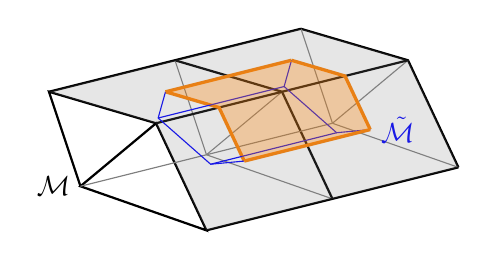
\begin{tikzpicture}[scale=0.8]
            \coordinate (A1) at (0,0);
            \coordinate (A2) at (2,-0.7);
            \coordinate (A3) at (1.2,1);
            \coordinate (A4) at (-0.5,1.5);
            \draw[thick] (A1) node[left] {$\mathcal{M}$} -- (A2) -- (A3) -- cycle;
            \draw[thick] (A1) -- (A4) -- (A3);
            \begin{scope}[shift={(2,0.5)}]
                \coordinate (B1) at (0,0);
                \coordinate (B2) at (2,-0.7);
                \coordinate (B3) at (1.2,1);
                \coordinate (B4) at (-0.5,1.5);
                \draw[thick] (B2) -- (B3) -- (B4);
                \draw[gray]  (B1) -- (B3);
                \draw[gray]  (B1) -- (B2);
                \draw[gray]  (B1) -- (B4);
            \end{scope}
            \begin{scope}[shift={(4,1)}]
                \coordinate (C1) at (0,0);
                \coordinate (C2) at (2,-0.7);
                \coordinate (C3) at (1.2,1);
                \coordinate (C4) at (-0.5,1.5);
                \draw[thick] (C2) -- (C3) -- (C4);
                \draw[gray]  (C1) -- (C3);
                \draw[gray]  (C1) -- (C2);
                \draw[gray]  (C1) -- (C4);
            \end{scope}
            \draw[thick] (A4) -- (B4) -- (C4);
            \draw[thick] (A3) -- (B3) -- (C3);
            \draw[thick] (A2) -- (B2) -- (C2);
            \draw[gray]  (A1) -- (C1);
            \coordinate (O1) at (barycentric cs:A3=1,B3=1);
            \coordinate (O2) at (barycentric cs:A3=1,B3=1,A4=1,B4=1);
            \coordinate (O5) at (barycentric cs:A3=1,B3=1,A2=1,B2=1);
            \draw[orange, very thick] (O2) -- (O1) -- (O5);
            \coordinate (O3) at (barycentric cs:A1=1,A3=1,A4=1,B1=1,B3=1,B4=1);
            \coordinate (O4) at (barycentric cs:A1=1,A2=1,A3=1,B1=1,B2=1,B3=1);
            \draw[blue] (O2) -- (O3) -- (O4) -- (O5);
            \coordinate (OO1) at ([shift={(2,0.5)}]O1);
            \coordinate (OO2) at ([shift={(2,0.5)}]O2);
            \coordinate (OO3) at ([shift={(2,0.5)}]O3);
            \coordinate (OO4) at ([shift={(2,0.5)}]O4);
            \coordinate (OO5) at ([shift={(2,0.5)}]O5);
            \draw[very thick, orange] (OO2) -- (OO1) -- (OO5) node[right] {\textcolor{blue}{$\Tilde{\mathcal{M}}$}};
            \draw[blue] (OO2) -- (OO3) -- (OO4) -- (OO5);
            \draw[very thick, orange] (O2) -- (OO2);
            %\draw[very thick, blue] (O1) -- (OO1);
            \draw[very thick, orange] (O5) -- (OO5);
            \draw[blue] (O3) -- (OO3);
            \draw[blue] (O4) -- (OO4);
            \fill[gray,opacity=0.2] (A4) -- (A3) -- (C3) -- (C4);
            \fill[gray,opacity=0.2] (A3) -- (A2) -- (C2) -- (C3);
            \fill[orange,opacity=0.3] (OO2)--(O2)--(O1)--(O5)--(OO5)--(OO1);
        \end{tikzpicture}
        \caption{3D case}
    \end{subfigure}
    \caption{Illustration of cut-off boundary. Before the cut-off, the boundary of $\Tilde{\mathcal{M}}$ is not well-defined. To resolve the same boundary as $\mathcal{M}$, boundary dual cells are truncated and auxiliary entities are supplemented (shown in orange color). To be specific, in subfigure (c) four edges and one face are added in order to close this dual cell. Notice that these auxiliary edges and faces can be non-straight and non-flat.}
    \label{fig:illustraion_dual_boundary}
\end{figure}

A pair of primal and dual meshes for the geometry in Fig. \ref{fig:domain_sketch} is displayed in Fig. \ref{fig:primal_dual_meshes}.

\subsection{Discrete Maxwell Equations}
\subsubsection{Finite Integration Technique (FIT)} \label{sec:fit}

We utilize FIT to discretize Maxwell's equations. This framework was originally proposed
in \cite{weiland_1977} and can be regarded as a generalization of Yee's FDTD method
\cite{yee_1966}. To derive a discrete model for the (rescaled) Maxwell equations
(\ref{equ:maxwell_faraday_rescaled})-(\ref{equ:maxwell_gauss_D_rescaled}), we first cast 
them into integral form: 
\begin{subequations}
\begin{align}
    &\oint_{\partial A} \mathbf{E} \cdot \text{d}\mathbf{s} \ = - \iint_A {\partial_t \mathbf{B}} \cdot \text{d}\mathbf{A}, \label{equ:maxwell_int_faraday}\\
    &\oint_{\partial A} \mathbf{H} \cdot \text{d}\mathbf{s} \ = \iint_A \left({\lambda^2\partial_t \mathbf{D}} + \mathbf{J}\right) \cdot \text{d}\mathbf{A}, \label{equ:maxwell_int_ampere}\\
    &\oint_{\partial V} \mathbf{B} \cdot \text{d}\mathbf{A} = 0, \label{equ:maxwell_int_gauss_B}\\
    &\oint_{\partial V} \lambda^2\mathbf{D} \cdot \text{d}\mathbf{A} = \iiint_V \rho \text{d}V. \label{equ:maxwell_int_gauss_D}
\end{align}
\end{subequations}
where $A, V$ stand for arbitrary surfaces and cells in the spatial domain. 

Given the mesh pair $(\mathcal{M}, \Tilde{\mathcal{M}})$, the discrete Maxwell system
arises from restricting the integrals
(\ref{equ:maxwell_int_faraday})-(\ref{equ:maxwell_int_gauss_D}) to the entities in
$(\mathcal{M}, \Tilde{\mathcal{M}})$. We end up with
\begin{subequations}
\begin{align}
    \sum_{k:L_k\in\partial A_l} \underbrace{\int_{L_k} \mathbf{E} \cdot \text{d}\mathbf{s}}_{:= e_k} &= - {\partial_t} \underbrace{\iint_{A_l} \mathbf{B} \cdot \text{d}\mathbf{A}}_{:= b_l},&l = 1,...,N_A, \label{equ:maxwell_grid_faraday} \\
    \sum_{k:\Tilde{L}_k\in\partial \Tilde{A}_l} \underbrace{\int_{\Tilde{L}_k} \mathbf{H} \cdot \text{d}\mathbf{s}}_{:= h_k} &= \lambda^2{\partial_t} \underbrace{\iint_{\Tilde{A}_l} \mathbf{D} \cdot \text{d}\mathbf{A}}_{:= d_l} + \underbrace{\iint_{\Tilde{A}_l} \mathbf{J} \cdot \text{d}\mathbf{A}}_{:= j_l}, &l = 1,...,N_{\Tilde{A}}, \label{equ:maxwell_grid_ampere}\\
    \sum_{k:A_k\in \partial V_l} \iint_{A_k} \mathbf{B} \cdot \text{d}\mathbf{A} &= 0,&l = 1,..., N_V,\label{equ:maxwell_grid_gauss_B}\\
    \lambda^2\sum_{k:\Tilde{A}_k \in \partial\Tilde{V}_l}\iint_{\Tilde{A}_k} \mathbf{D} \cdot \text{d}\mathbf{A} &= \underbrace{\iiint_{\Tilde{V}_l} \rho \text{d}V}_{:= q_l},&l = 1,...,N_{\Tilde{V}}. \label{equ:maxwell_grid_gauss_D}
\end{align}
\end{subequations}
where $k, l$ number the entities in $(\mathcal{M}, \Tilde{\mathcal{M}})$.  The integral
field quantities are the unknowns of the discrete Maxwell model. As is defined in
(\ref{equ:maxwell_grid_faraday})-(\ref{equ:maxwell_grid_gauss_D}) by the underbraces,
these unknowns are stacked into vectors:
\begin{equation}
  \label{equ:fit_scale_vector}
  \mathbf{e} := \{e_k\}_{k=1}^{N_L},\ \ \mathbf{b} := \{b_k\}_{k=1}^{N_A}, \ \ \mathbf{h} := \{h_k\}_{k=1}^{N_{\Tilde{L}}}, \ \ \mathbf{d} := \{d_k\}_{k=1}^{N_{\Tilde{A}}}, \ \ \mathbf{j} := \{j_k\}_{k=1}^{N_{\Tilde{A}}}, \ \ \mathbf{q} := \{q_k\}_{i=k}^{N_{\Tilde{V}}}.
\end{equation}

\begin{remark}
    In an implementation, it is always convenient to index a pair of corresponding primal and dual entities with the same number. For instance, a primal face $A_k$ is penetrated by the dual edge $\Tilde{L}_k$. In the following discussion, we stick to this convention, which will simplify our notation.
\end{remark}

The material laws (\ref{equ:material_law}) need to be taken into account within this
framework, that is, relations $\mathbf{b} = \mathbb{M}_\mu \mathbf{h}$ and $\mathbf{d} =
\mathbb{M}_\epsilon \mathbf{e}$ with suitable \emph{material} matrices $\mathbb{M}_\mu,
\mathbb{M}_\epsilon$. When the orthogonality of the pair ($\mathcal{M},
\Tilde{\mathcal{M}}$) holds, the discrete material laws can consistently be represented by
\emph{diagonal matrices} with entries
\begin{equation*}
    (\mathbb{M}_\mu)_{k,k} = \frac{\mu|A_k|}{|\Tilde{L}_k|}, \ \ \ \ \ (\mathbb{M}_\epsilon)_{k,k} = \frac{\epsilon |\Tilde{A}_k|}{|L_k|},
\end{equation*}
where $|\cdot|$ denotes taking length or area. We would like to remark that an
approximation error is introduced due to the implicit assumption that vector fields are
piecewise constant, see the analysis in \cite[][Sec. 3.2]{Marrone_2001}.

With the aid of incidence matrices defined in the preceding section and given the discrete
material law, (\ref{equ:maxwell_grid_faraday})-(\ref{equ:maxwell_grid_gauss_D}) can be
recast into a set of algebraic equations:
\begin{center}
\vspace{-0.5cm}
\begin{minipage}{0.3\textwidth}
\begin{align*}
    \partial_t \mathbf{B} + \nabla \times \mathbf{E} &= 0, \\
    \lambda^2\partial_t \mathbf{D} - \nabla \times \mathbf{H} &= -\mathbf{J}, \\
    \nabla \cdot \mathbf{B} &= 0,  \\
    \lambda^2\nabla \cdot \mathbf{D} &= \rho, \\
    \mathbf{H} &= \mu^{-1} \mathbf{B}, \\
    \mathbf{D} &= \epsilon \mathbf{E}. 
\end{align*}
\end{minipage}
\begin{minipage}{0.1\textwidth}
\centering
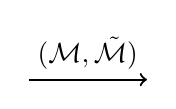
\begin{tikzpicture}
\draw[thick, -{to}] (0,0) -- node[above]{$(\mathcal{M}, \Tilde{\mathcal{M}})$} (1.5,0);
\end{tikzpicture}
\end{minipage}
\begin{minipage}{0.3\textwidth}
\begin{subequations}
\begin{align}
    \dot{\mathbf{b}} + \mathbb{C}\mathbf{e} &= \mathbf{0} , \label{equ:alg_faraday}\\
    \lambda^2\dot{\mathbf{d}} - \Tilde{\mathbb{C}}\mathbf{h} &= - \mathbf{j}, \label{equ:alg_empere}\\
    \mathbb{D}\mathbf{b} &= \mathbf{0},  \label{equ:alg_gauss_b}\\
    \lambda^2\Tilde{\mathbb{D}}\mathbf{d} &= \mathbf{q},  \label{equ:alg_gauss_d}\\
    \mathbf{h} &= \mathbb{M}_\mu^{-1} \mathbf{b}, \label{equ:alg_material_magnetic}\\
    \mathbf{d} &= \mathbb{M}_{\epsilon} \mathbf{e}, \label{equ:alg_material_electric} 
\end{align}
\end{subequations}
\end{minipage}
\end{center}
where the dot on top of quantities stands for the time derivative.

\begin{remark}
  At this point, we would like to emphasize the importance of the primal-dual staggered
  meshes: \emph{the material laws can be included in a rather simple way.} For Gauss's law
  $\mathbf{D} = \epsilon \mathbf{E}$, for instance, the $\mathbf{D}$-field is represented
  by a collection of face integrals $ \{d_k\}_{k}$ while the $\mathbf{E}$-field is
  represented by a collection of edge integrals $ \{e_k\}_{k}$. The primal-dual meshes
  allow us to arrange them in a staggered way -- edges penetrate faces -- such that
  $\mathbf{D} = \epsilon \mathbf{E}$ can be approximated by
  $\mathbf{d} = \mathbb{M}_{\epsilon}\mathbf{e}$ in a local fashion,
  i.e. $\mathbb{M}_{\epsilon}$ is diagonal. A more schematic illustration relies on the
  language of discrete exterior calculus (DEC), see \cite{bossavit1999, teixeira_1999,
    hip_1999}.
\end{remark}

Summing up, the essence of DEC/FIT is the following:
\begin{enumerate}[label={(\roman{*})}]
\item The discrete Maxwell model (\ref{equ:alg_faraday})-(\ref{equ:alg_gauss_d}) are
  topological in the sense that they are invariant under different coordinate
  systems. Only the discrete material laws
  (\ref{equ:alg_material_magnetic})(\ref{equ:alg_material_magnetic}) depend on the
  geometric information.
\item The discrete Maxwell model (\ref{equ:alg_faraday})-(\ref{equ:alg_gauss_d}) is free
  of approximation error, that is, it holds for exact fields. A consistency error is
  introduced only by the discrete material laws
  (\ref{equ:alg_material_magnetic})(\ref{equ:alg_material_magnetic}).
\end{enumerate}

\subsubsection{Discrete Boundary Conditions}

The electromagnetic boundary $\partial\Omega = \Gamma_C\cup \Gamma_I$ is resolved by the
primal mesh $\mathcal{M}$. As is mentioned in Section \ref{sec:BC}, the zero-magnetic-flux
boundary condition $\mathbf{B}\cdot \mathbf{n}$ is equivalent to
$(\nabla\times\mathbf{E}) \cdot \mathbf{n} = 0$, which paves the way for a surface scalar
potential $\varphi:\partial\Omega\to\mathbb{R}$ such that the tangential component
$\mathbf{E}_t$ of the $\mathbf{E}$-field is equal to $\nabla_\Gamma\varphi$. This remains
true on the discrete level. We associate with each primal vertex $P_k \in \partial\Omega$
a scalar value $\varphi_k$. Therefore, the boundary conditions (see Section \ref{sec:BC})
are discretized in the following way:
\begin{center}
    \vspace{-0.5cm}
    \begin{minipage}{0.3\textwidth}
    \begin{align*}
    \mathbf{D} \cdot \mathbf{n} = 0\ \ &\text{on} \ \  \Gamma_I,  \\
    \mathbf{B} \cdot \mathbf{n} = 0\ \  &\text{on} \ \  \Gamma_I, \\
    \varphi = \varphi^\pm(t)\ \ &\text{on} \ \ \Gamma_C^\pm,
    \end{align*}
    \end{minipage}
    \begin{minipage}{0.1\textwidth}
    \centering
    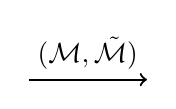
\begin{tikzpicture}
    \draw[thick, -{to}] (0,0) -- node[above]{$(\mathcal{M}, \Tilde{\mathcal{M}})$} (1.5,0);
    \end{tikzpicture}
    \end{minipage}
    \begin{minipage}{0.5\textwidth}
        \centering
        \begin{subequations}
            \begin{align}
            d_k = 0,\ \ &\forall k : \Tilde{A}_k \subset \Gamma_I,\label{equ:bc_3} \\
            e_k = (\mathbb{GX}_\varphi\bm{\varphi})_k,\ \ &\forall k : L_k \subset \partial\Omega, \label{equ:bc_2}\\
            \varphi_k = \varphi^\pm(t), \ \ &\forall k : P_k \subset \Gamma_C^\pm, \label{equ:bc_1}
            \end{align}
        \end{subequations}
    \end{minipage}
\end{center}
where $\mathbb{X}_\varphi \in \mathbb{R}^{N_P \times N_P^\partial}$ extends $\bm{\varphi}$
to all the primal verices by zero. Obviously, the surface gradient $\nabla_\Gamma$ is
represented by $\mathbb{GX}_\varphi$.

\subsubsection{Stabilization in $\Omega_N$} \label{sec:reform-discrete}

In Section \ref{sec:reform_continuous}, we have proposed a stabilization of the Maxwell
system in the non-conducting domain $\Omega_N$ by introducing a Lagrange multiplier. On
the semi-discrete level, the equations to be solved in $\Omega_N$ are
\begin{center}
    \begin{minipage}{0.3\textwidth}
    \begin{align*}
        \partial_t \mathbf{B} + \nabla \times \mathbf{E} &= 0, \\ 
        \lambda^2 \partial_t \mathbf{D} - \nabla \times \mathbf{H} + \colorbox{orange!20}{$\nabla \psi$} &= 0, \\
        \nabla \cdot \mathbf{D} &= 0. 
    \end{align*}
    \end{minipage}
    \begin{minipage}{0.1\textwidth}
    \centering
    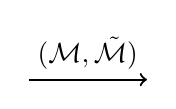
\begin{tikzpicture}
    \draw[thick, -{to}] (0,0) -- node[above]{$(\mathcal{M}, \Tilde{\mathcal{M}})$} (1.5,0);
    \end{tikzpicture}
    \end{minipage}
    \begin{minipage}{0.5\textwidth}
        \begin{subequations}
        \begin{align}
            [\dot{\mathbf{b}} + \mathbb{C}\mathbf{e} &= \mathbf{0}]_k,\ \ \forall k:A_k \subset \Omega_N,\\
            [\lambda^2\dot{\mathbf{d}} - \Tilde{\mathbb{C}}\mathbf{h} + \colorbox{orange!20}{$\mathbb{H} \mathbb{G} \mathbb{X}_\psi \bm{\psi}$}&= \mathbf{0}]_k, \ \ \forall k: \Tilde{A}_k \subset \Omega_N \label{equ:discrete_ampere_ins}\\
            [\Tilde{\mathbb{D}}\mathbf{d} &= \mathbf{0}]_k,\ \ \forall k:\Tilde{V}_k \subset \Omega_N \label{equ:discrete_zero_div}, 
        \end{align} 
    \end{subequations}
    \end{minipage}
\end{center}
where $\bm{\psi} := \{\psi_k\}_{k=1}^{N_P^N}$ denotes unknowns assigned to each primal
vertex in $\Omega_N$. The matrix $\mathbb{X}_\psi \in \mathbb{R}^{N_P \times N_P^{N}}$
extends $\bm{\psi}$ by zero to all the primal vertices. This way the zero Dirichlet
boundary condition is incorporated. We need the diagonal matrix
$(\mathbb{H})_{k,k} = {|\Tilde{A}_k|}/{|L_k|}$ to transform primal edge integrals to dual
face fluxes since the discrete Amp\`{e}re's law (\ref{equ:discrete_ampere_ins}) is defined
on dual faces on $\Omega_N$.

\subsubsection{Numbers of Equations and Unknowns}

We can probe the well-posedness of the (semi-)discrete Maxwell system by checking whether
the numbers of unknowns (also called degrees of freedom (D.o.F.)) and equations coincide.
First, we count mesh entities according to their locations:
\begin{center}
\vspace{-0.5cm}
\begin{minipage}[t]{0.4\textwidth}
    \begin{align*}
        &\#\  \text{primal cells}\ \  N_V, \\
        &\#\  \text{primal edges}\ \  N_L := \underbrace{N^C_L + N^I_L}_{=N^\partial_L} + N^\circ_L,  \\
        &\#\  \text{primal faces}\ \  N_A := \underbrace{N_A^C + N^I_A}_{=N^\partial_A} + N^\circ_A , \\
        &\#\  \text{primal vertices}\ \  N_P := \underbrace{N_P^C + N^I_P}_{=N^\partial_P} + N^\circ_P,
    \end{align*}
\end{minipage}
\begin{minipage}[t]{0.4\textwidth}
    \begin{align*}
        &\#\  \text{dual cells}\ \  N_{\Tilde{V}} := N_P ,\\
        &\#\  \text{dual edges}\ \  N_{\Tilde{L}} := \underbrace{N^\partial_{\Tilde{L}}}_{=N^\partial_L} + \underbrace{N^\circ_{\Tilde{L}}}_{=N_A} ,\\
        &\#\  \text{dual faces}\ \  N_{\Tilde{A}} := \underbrace{N^\partial_{\Tilde{A}}}_{=N^\partial_P} + \underbrace{N^\circ_{\Tilde{A}}}_{=N_L},
    \end{align*}
\end{minipage}   
\end{center}
where the superscripts indicate where the entities are located. The equalities
$N^\partial_{\Tilde{L}} = N^\partial_L, N^\partial_{\Tilde{A}} = N^\partial_P$ reveal the
bijective relation between the boundary primal entities and auxiliary entities, as can be
checked easily by inspecting Fig.~\ref{fig:illustraion_dual_boundary}.  We also give a
summary of the unknowns in Tab.~\ref{tab:def_size_var}.
\begin{table}[]
    \centering
\begin{tabular}{c c c}
     \hline
     Vector of unknowns  & Meaning  & Vector size \\
     \hline
     $\mathbf{e}$ & line integrals of $\mathbf{E}$-field at primal edges $L$& $N_L$ \\
     $\bm{\varphi}$ & boundary scalar potential $\varphi$ at primal vertices $P$ on $\partial\Omega$ & $N_P^\partial$ \\
     $\mathbf{b}$ & surface integrals of $\mathbf{B}$-field at primal faces $A$ & $N_A$ \\
     $\mathbf{h}$ & line integrals of $\mathbf{H}$-field at dual edges $\Tilde{L}$ & $N_{\Tilde{L}}$ \\
     $\mathbf{d}$ & surface integrals of $\mathbf{D}$-field at dual faces $\Tilde{A}$ & $N_{\Tilde{A}}$ \\
     $\bm{\psi}$ & Lagrange multiplier $\psi$ at primal vertices $P$ in $\Omega_N$ & $N^{N}_P$\\ 
     \hline
\end{tabular}
    \caption{Definitions and sizes of the vectors of unknowns.}
    \label{tab:def_size_var}
\end{table}

Next, we collect all the algebraic equations derived from the Maxwell system and the boundary conditions: 
\begin{align*}
    \text{discrete Faraday's law (\ref{equ:alg_faraday})} \ \ &\longrightarrow\ \  N_A \ \ \text{equations} \\
    \text{discrete Ampere's law (\ref{equ:alg_empere})} \ \ &\longrightarrow\ \  N_{\Tilde{A}} \ \ \text{equations} \\
    \text{discrete material laws (\ref{equ:alg_material_magnetic})(\ref{equ:alg_material_electric})} \ \ &\longrightarrow\ \  N_A + N_L \ \ \text{equations} \\
    \text{boundary condition (\ref{equ:bc_1})} \ \ &\longrightarrow\ \  N_P^C \ \ \text{equations} \\
    \text{boundary condition (\ref{equ:bc_2})} \ \ &\longrightarrow\ \  N_L^\partial \ \ \text{equations} \\
    \text{boundary condition (\ref{equ:bc_3})} \ \ &\longrightarrow\ \  N_{\Tilde{A}}^I \ \ \text{equations}. \\
    \text{vanishing divergence constraint (\ref{equ:discrete_zero_div})} \ \ &\longrightarrow\ \  N_{\Tilde{V}}^{N} \ \ \text{equations}. \\
\end{align*}
Comparing the numbers of d.o.f. in Tab.~\ref{tab:def_size_var} and of the equations we
collect above, we see that they are equal:
\begin{align*}
    \#\text{ of unknowns} &= \colorbox{violet!20}{$N_L$} + \colorbox{blue!20}{$N_A$} + \colorbox{gray!40}{$N_{\Tilde{L}}$} + \colorbox{orange!20}{$N_{\Tilde{A}}$} + \colorbox{green!20}{$N_P^\partial$} + \colorbox{yellow!40}{$N_P^{N}$}, \\
    \#\text{ of equations} &= \colorbox{blue!20}{$N_A$} + \colorbox{orange!20}{$N_{\Tilde{A}}$} + \colorbox{gray!40}{$N_A+N_L^\partial$} + \colorbox{violet!20}{$N_L$} + \colorbox{green!20}{$N_P^C + N_P^I$}+ \colorbox{yellow!40}{$N_{\Tilde{V}}^N$}.
\end{align*}
Of course, the matching numbers of unknowns and equations do not necessarily result in a
valid linear system, since the equations might be linearly dependent. In fact, the linear
system will be singular without the stabilization proposed in the previous section when
$\lambda = 0$.

\subsection{Discrete Euler Equations} \label{sec:discrete_euler}

We employ the finite volume method (FVM) to discretize the Euler system. The Euler
equations (\ref{equ:euler_}) can be cast into the form of conservation law with source
terms:
\begin{equation} \label{equ:euler_conservation}
    \partial_t \mathbf{U} + \nabla \cdot \mathbf{f}(\mathbf{U}) = \mathbf{RHS},
\end{equation}
where $\mathbf{U} \in L^2(\Omega \times [0,T], \mathbb{R}^m)$ stands for a vector of $m$
conservative variables,
$\mathbf{f}(\mathbf{U}) \in L^2(\Omega \times [0,T], \mathbb{R}^{3 \times m})$ is the flux
function, and $\mathbf{RHS} \in L^2(\Omega \times [0,T], \mathbb{R}^m)$ is the source
term.. In the case of the full 3D Euler equations (\ref{equ:euler_rescaled}), $m = 5$ and
$\mathbf{U} := [n, n\mathbf{u}, ne]$.

To obtain the semi-discretization, we first integrate (\ref{equ:euler_conservation}) over
a \emph{dual} cell $\Tilde{V}_k \in \Omega_P$
\begin{equation} \label{equ:euler_grid} 
    \dot{\overline{\mathbf{U}}}_k + \frac{1}{|\Tilde{V}_k|}\sum_{l:\Tilde{A}_l\in\partial \Tilde{V}_k} |\Tilde{A}_l|\underbrace{\frac{1}{|\Tilde{A}_l|}\iint_{\Tilde{A}_l}\mathbf{f}(\mathbf{U})\cdot \mathbf{n}_l \text{d}A}_{:= \overline{\mathbf{f}}_l \approx \mathbf{f}^\text{num}_l} = \underbrace{\frac{1}{|\Tilde{V}_k|}\iiint_{\Tilde{V}_k} \mathbf{RHS} \text{d}V}_{:= \overline{\mathbf{RHS}}_k},\ \ k = 1,2,\cdots,N_{\Tilde{V}}^P
\end{equation}
where
$\overline{\mathbf{U}}_k := \iiint_{\Tilde{V}_k} \mathbf{U} \text{d}V / |\Tilde{V}_k| \in
L^2([0,T],\mathbb{R}^m)$ is the cell average of $\mathbf{U}$ and $\mathbf{n}_l$ is the
outer normal vector of face $\Tilde{A}_l$ with respect to the cell $\Tilde{V}_k$. In FVM,
the flux $\overline{\mathbf{f}}_l$ in (\ref{equ:euler_grid}) is approximated by a
numerical flux
$\mathbf{f}^\text{num}_l := \mathbf{f}^\text{num}\left(\overline{\mathbf{U}}_k,
  \overline{\mathbf{U}}_{\hat{k}(k,l)}, \mathbf{n}_l\right)$, where $\hat{k}(k,l)$ returns
the index of the adjacent dual cell that shares $\Tilde{A}_l$ with cell
$\Tilde{V}_k$. Classical numerical fluxes include the Lax-Friedrich flux, the Rusanov
flux, and the Engquist-Osher flux, see \cite[][pp. 44-46]{mishra_2019}. We end up with the
semi-discretized equation:
\begin{equation}
  \dot{\overline{\mathbf{U}}}_k + \frac{1}{|V_k|}\sum_{l:\Tilde{A}_l\in\partial \Tilde{V}_k} |\Tilde{A}_l| \mathbf{f}^\text{num}\left(\overline{\mathbf{U}}_k, \overline{\mathbf{U}}_{\hat{k}(k,l)}, \mathbf{n}_l\right) = \overline{\mathbf{RHS}}_k,\ \  k = 1,2,\cdots,N_{\Tilde{V}}^P.
    \label{equ:fvm}
\end{equation}
We employ the Rusanov flux, which writes
\begin{equation} \label{equ:rusanov-flux-3d}
    \mathbf{f}^\text{num}\left(\overline{\mathbf{U}}_L, \overline{\mathbf{U}}_R, \mathbf{n}\right) = \frac{1}{2}\left[\mathbf{f}(\overline{\mathbf{U}}_L)\cdot\mathbf{n} + \mathbf{f}(\overline{\mathbf{U}}_R)\cdot\mathbf{n}\right] - \frac{1}{2}\overline{s}\left(\overline{\mathbf{U}}_R - \overline{\mathbf{U}}_L\right),  
\end{equation}
where $\overline{s} = \text{max}\{s(\overline{\mathbf{U}}_L), s(\overline{\mathbf{U}}_R)\}$ with $s(\mathbf{U}) := |\mathbf{u}\cdot\mathbf{n}| + \sqrt{\gamma p/\rho}$ representing the largest wave speed. 

At this stage, we would like to discuss why \emph{the Euler system should be discretized
  on $\Tilde{\mathcal{M}}$}. As is shown in the integrated Amp\`{e}re's law
(\ref{equ:maxwell_int_ampere}), the electric currents are defined on dual faces
$\Tilde{A}$. By solving the Euler equations on $\Tilde{\mathcal{M}}$, we have the mass
flux on dual faces $\Tilde{A}$ as well. In this way, the connection between the charge
conservation (\ref{equ:charge_continuity}) and the mass conservation (the 1st equation in
(\ref{equ:euler_})) due to the current-momentum coupling
(\ref{equ:maxwell_euler_coupling}) is preserved on the discrete level.

For the sake of presentation, we rewrite (\ref{equ:fvm}) into a matrix form. By abuse of
notation, we stack all the cell average
$\{\overline{\mathbf{U}}_k\}_{k=1}^{N^P_{\Tilde{V}}}$ into a matrix
$\mathbf{U} \in \mathbb{R}^{N_{\Tilde{V}}^P \times 5}$ with
$\mathbf{U}_{k,:} = \overline{\mathbf{U}}_k$. Further, we denote by
$\mathbf{F} \in \mathbb{R}^{N_{\Tilde{A}}^P \times 5}$ the collection of the (total)
numerical fluxes, i.e.
$\mathbf{F}_{k,:} = \mathbf{f}^\text{num}_k = [f^\text{mass}_k, \bm{f}^\text{mom}_k,
f^\text{ene}_k]$. In the same way, we denote by
$\mathbf{RHS}\in \mathbb{R}^{N_{\Tilde{V}}^P \times 5}$ the collection of
$\overline{\mathbf{RHS}}_k$. Besides, we define the diagonal matrices
$\mathbb{\Tilde{V}} \in \mathbb{R}^{N_{\Tilde{V}}^P \times N_{\Tilde{V}}^P}$ and
$\mathbb{\Tilde{A}}\in \mathbb{R}^{N_{\Tilde{A}}^P \times N_{\Tilde{A}}^P}$ with
$(\mathbb{\Tilde{A}})_{k,k} = |\Tilde{A}_k|$. Making use of the incidence matrices, we end
up with
\begin{equation} \label{equ:euler_matrix_form}
    \dot{\mathbf{U}} + \mathbb{\Tilde{V}}^{-1}\mathbb{\Tilde{D}}\mathbb{\Tilde{A}}\mathbf{F}(\mathbf{U})  = \mathbf{RHS}(\mathbf{U},\mathbf{d},\mathbf{b}),
\end{equation}
Recall that $\Tilde{\mathbb{D}}$ represents the discrete divergence of
$\Tilde{\mathcal{M}}$. Dependence of $\mathbf{RHS}$ on $\mathbf{d}, \mathbf{b}$ is implied
by (\ref{equ:euler_rescaled}) and will be elaborated next.

\subsubsection{Reconstruction of Lorentz Force}

Since the electromagnetic fields are represented by integrals on edges and faces, we need
to reconstruct their vector components for the computation of Lorentz force (and Joule
heating) inside each dual cell. The task involves two aspects:
\begin{itemize}
    \item[-] given the fluxes at the faces of a cell, reconstruct the vector field inside the cell;
    \item[-] given the integrals along the edges of a cell, reconstruct the vector field inside the cell. 
\end{itemize}
We adopt the principle of least square fitting and reconstruct a \emph{constant} vector
field inside each cell. For a cell $\Tilde{V}$ with $N_A$ faces with areas
$\{A_k\}_{k=1}^{N_A}$, normal vectors $\{\mathbf{n}_k\}_{k=1}^{N_A}$ and fluxes
$\{f_k\}_{k=1}^{N_A}$, a constant vector field $\mathbf{v}$ satisfying
\begin{equation*}
    \mathbf{v} = \argmin_{\mathbf{w}\in \mathbb{R}^3} \sum_{k=1}^{N_A}(A_k\mathbf{w} \cdot \mathbf{n}_k - f_k)^2.   
\end{equation*} can be computed through
\begin{equation*}
    \mathbf{v} = (\mathbb{K}^T\mathbb{K})^{-1}\mathbb{K}^T\mathbf{f},
\end{equation*}
where
\begin{equation*}
    \mathbb{K} = [A_1\mathbf{n}_1, A_2\mathbf{n}_2, \cdots, A_{N_A}\mathbf{n}_{N_A}]^T,\ \ \ \mathbf{f} = [f_1, f_2, \cdots, f_{N_A}]^T,
\end{equation*}
and each vector in $\mathbb{R}^3$ is treated as a column vector. The construction based on
the integral quantities on edges can be done similarly. Assembling the local constructions
for each dual cell, the global construction can be written as
\begin{equation}
    \mathbf{E} = \Tilde{\mathbb{R}}_E\mathbf{d}\;,
    \quad
    \mathbf{B} = \Tilde{\mathbb{R}}_B\mathbf{b},
    \label{equ:reconstruction}
\end{equation}
where $\mathbf{d}, \mathbf{b}$ are defined in Tab. \ref{tab:def_size_var};
$\mathbf{E} := \{\mathbf{E}_k\}_{k=1}^{N_{\Tilde{V}}}$ and
$\mathbf{B} := \{\mathbf{B}_k\}_{k=1}^{N_{\Tilde{V}}}$ are $N_{\Tilde{V}} \times 3$
matrices containing the reconstructed $\mathbf{E}$-fields and $\mathbf{B}$-fields at each
$\Tilde{V}$; $\Tilde{\mathbb{R}}_E$ and $\Tilde{\mathbb{R}}_B$ are thus rank-3 tensors.

The problem of the reconstruction of vector fields on unstructured meshes is a widely
studied topic. Apart from the least-square method, other methods include Perot's method
\citep{perot_2000}, finite-entity-based methods, etc., which potentially can achieve
higher-order accuracy. See \cite[][Sec. 3.4.4]{fuchs_2021} and the references therein.

Eventually, the right-hand-side term in (\ref{equ:euler_matrix_form}) can be computed by
evaluating the right-hand-side of rescaled Euler equations (\ref{equ:euler_rescaled}) for
the reconstructed $\mathbf{E}$-field and $\mathbf{B}$-field by (\ref{equ:reconstruction})
defined in each dual cell.

\subsubsection{Discrete Boundary Conditions}

The boundary conditions for the Euler system (see Section \ref{sec:BC}) are implemented by
the approach of ghost cells \cite[][Ch. 7]{leveque_2007}, i.e. extending the domain by a
layer of virtual cells with prescribed variables. In our case, the ghost cells at the open
boundary at $\Gamma_C$ are assigned the same state as their adjacent interior cells. It is
equivalent to enforcing the numerical fluxes
\begin{equation} \label{equ:discrete_open_bc}
    \mathbf{F}_k = {\mathbf{f}^\text{num}}(\mathbf{U}_l, \mathbf{U}_l, \mathbf{n}_k), \ \ \forall k: \Tilde{A}_k \subset \Gamma_C,
\end{equation}
where $l$ refers to the (unique!) index of the cell adjacent to the boundary face
$\Tilde{A}_k$. For the \emph{reflective wall} $\Gamma_W$, the momentum of a ghost cell is
reversed with respect to its adjacent interior cell while keeping the other quantities
unchanged. Therefore, in this case the numerical fluxes are
\begin{equation} \label{equ:discrete_wall_bc} \mathbf{F}_k =
  \mathbf{f}^\text{num}(\mathbf{U}_l, \hat{\mathbf{U}}_l, \mathbf{n}_k), \ \ \forall k:
  \Tilde{A}_k \subset \Gamma_W,
\end{equation}
where the state of the ghost cell
$\hat{\mathbf{U}}_l = [n, n\mathbf{u} - 2(\mathbf{n}\cdot\mathbf{u})\mathbf{n}, ne]^T$
reverses the normal velocity of $\mathbf{U}_l = [n, n\mathbf{u}, ne]^T$.


\subsection{Summary: Spatially Semi-discrete Model}
We collect all the equations and boundary conditions presented above and give a summary for the spatially semi-discrete Maxwell-Euler system based on the FIT/DEC-FVM framework:
\begin{subequations}
\begin{align}
    (\ref{equ:alg_faraday}) & \implies \;\;\;\;\;\;\;\;\;\;\;\;\;\;\;\;\;\;\;\;\;\;\;\;\;\;\;\;&  [\dot{\mathbf{b}} + \mathbb{C}\mathbf{e} = \mathbf{0}]_k, \ \ &\forall k: A_k \subset \Omega,  \;\;\;\;\;\;\;\;\;\;\;\;\;\;\;\;\;\;\;\;\;\;\;\;\;\;\;\;\;\;\;\;\;\;\;\;\;\;\;\;\;\;\;\; \label{equ:faraday_semi_discrete}\\
    (\ref{equ:alg_empere})  & \implies & [\dot{\mathbf{d}} - \Tilde{\mathbb{C}}\mathbf{h} = - \Sigma_{\ast} q_*\bm{f}_{\ast}^\text{mass}]_k, \ \ &\forall k: \Tilde{A}_k \subset \Omega_P, \label{equ:empere_semi_discrete}\\
    (\ref{equ:discrete_ampere_ins}) & \implies & [\dot{\mathbf{d}} - \Tilde{\mathbb{C}}\mathbf{h} + \mathbb{H} \mathbb{GX}_\psi \bm{\psi} = \mathbf{0}]_k, \ \ &\forall k: \Tilde{A}_k \subset \Omega_N, \label{equ:ampere_ins_semi_discrete}\\
    (\ref{equ:discrete_zero_div}) & \implies & [\Tilde{\mathbb{D}}\mathbf{d} = \mathbf{0}]_k,\ \ &\forall k: \Tilde{V}_k \subset \Omega_N, \label{equ:zero_div_ins_semi_discrete}\\
    (\ref{equ:euler_matrix_form}) & \implies & [\dot{\mathbf{U}}_\ast + \mathbb{\Tilde{V}}^{-1}\mathbb{\Tilde{D}}\mathbb{\Tilde{A}}\mathbf{F}_\ast = \mathbf{RHS}_\ast]_k,\ \ &\forall k: \Tilde{V}_i \subset \Omega_P, \label{equ:euler_semi_discrete} \\
     (\ref{equ:alg_material_magnetic}) & \implies & [\mathbf{h} = \mathbb{M}_\mu^{-1}\mathbf{b}]_k, \ \ &\forall k:A_k \subset \Omega, \label{equ:material_law_h_semi_discrete}\\
    (\ref{equ:alg_material_electric}) & \implies & [\mathbf{d} = \mathbb{M}_\epsilon\mathbf{e}]_k,\ \ &\forall k:L_k \subset \Omega \label{equ:material_law_d_semi_discrete},
\end{align}
where $\ast \in \{e, i, \dots\}$ and $\bm{f}^\text{mass}$ denotes the mass flux which is defined in Section \ref{sec:discrete_euler}. By $[\cdots]_k$ we mean taking the $k$-th component of both sides of the equation. We have the following boundary conditions:
    \begin{align}
    (\ref{equ:bc_3}) & \implies \;\;\;\;\;\;\;\;\;\;\;\;\;\;\;\;\;\;\;\;\;\;\;\;\;\;\;\;& d_k = 0,\ \ &\forall k : \Tilde{A}_k \subset \Gamma_I,\;\;\;\;\;\;\;\;\;\;\;\;\;\;\;\;\;\;\;\;\;\;\;\;\;\;\;\;\;\;\;\;\;\;\;\;\;\;\;\;\;\;\;\;\\
    (\ref{equ:bc_2}) & \implies & e_k = (\mathbb{GX}_\varphi\bm{\varphi})_k,\ \ &\forall k : L_k \subset \partial\Omega, \\
    (\ref{equ:bc_1}) & \implies & \varphi_k = \varphi^\pm(t), \ \ &\forall k : P_k \subset \Gamma_C^\pm, \\ 
    (\ref{equ:discrete_open_bc}) & \implies & \mathbf{F}_{\ast,k} = \mathbf{f}^\text{num}(\mathbf{U}_{\ast,l}, \mathbf{U}_{\ast,l}, \mathbf{n}_k), \ \ &\forall k: \Tilde{A}_k \subset \Gamma_C, \\
    (\ref{equ:discrete_wall_bc}) & \implies & \mathbf{F}_{\ast,k} = \mathbf{f}^\text{num}(\mathbf{U}_{\ast,l}, \hat{\mathbf{U}}_{\ast,l}, \mathbf{n}_k), \ \ &\forall k: \Tilde{A}_k \subset \Gamma_W.
    \end{align}
\end{subequations}

We would like to stress again that in our FIT/DEC-FVM framework Faraday's law is
discretized on the primal mesh $\mathcal{M}$ while Amp\`{e}re's law is discretized on the
dual mesh $\Tilde{\mathcal{M}}$. The material laws directly connect primal and dual
d.o.f. Using the cells of the dual mesh $\Tilde{\mathcal{M}}$ as finite-volumes for the
Euler system the connection between electric currents and fluid momenta is perfectly
represented in the discretization, since both are defined on the dual faces.

\section{Full Discretization} \label{sec:full-discretization}
\subsection{Motivation: Reduction to One Spatial Dimension}

Our work extends the 1D scheme proposed in \cite{degond_2012} to three
dimensions. Therefore, it is supposed to be compatible with the original 1D scheme when
``projected'' to one dimension. This perspective helps to understand how the 3D scheme
is linked to the 1D. For the sake of presentation, we discuss the one-fluid model of
\cite{degond_2012}, for which ions are assumed immobile and only the motion of electrons is
considered.

\subsubsection{Projection to One Dimension} \label{sec:projection_to_1d}

Consider a primal-dual mesh pair $(\mathcal{M}, \Tilde{\mathcal{M}})$ that is constructed by 2D
extrusion along the $z$-axis and is unbounded in transverse directions. Assuming
transverse translation invariance and rotational symmetry, we can ``project'' all the d.o.f. onto the
$z$-axis. The idea is sketched in in Fig.~\ref{fig:1d_reduction}.

\begin{figure}
    \centering
    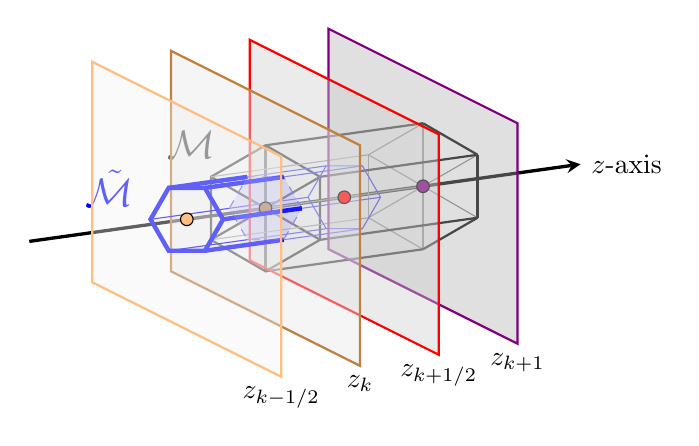
\begin{tikzpicture}[scale=0.4]
        \def\primalstyle{thick}
        \def\dualstyle{thick}
        \coordinate (P0) at (0cm, 0cm);
        \foreach \i in {1,2,...,6}
        {
        \coordinate (P\i) at ({60*\i-30}:2cm);
        \draw[\primalstyle] (P0) -- (P\i);
        }
        \draw[\primalstyle] (P1) -- (P2) node[left=5mm]{\Large $\mathcal{M}$} -- (P3) -- (P4) -- (P5) -- (P6) -- cycle;
        
        \draw[very thick, -stealth] (-7.5,-1.05) -- (10,1.4) node[right] {$z$-axis};
        \begin{scope}[shift={(5cm,0.7
        cm)}]
            \coordinate (PP0) at (0cm, 0cm);
            \foreach \i in {1,2,...,6}
            {
            \coordinate (PP\i) at ({60*\i-30}:2cm);
            \draw[gray] (PP0) -- (PP\i);
            }
        \end{scope}

        
        \draw[\primalstyle] (PP1) -- (PP2);
        \draw[gray] (PP2) -- (PP3);
        \draw[gray] (PP3) -- (PP4);
        \draw[gray] (PP4) -- (PP5);
        \draw[\primalstyle] (PP5) -- (PP6);
        \draw[\primalstyle] (PP6) -- (PP1);
        
        \draw[gray] (P0) -- (PP0);
        \draw[\primalstyle] (P1) -- (PP1);
        \draw[\primalstyle] (P2) -- (PP2);
        \draw[gray] (P3) -- (PP3);
        \draw[gray] (P4) -- (PP4);
        \draw[\primalstyle] (P5) -- (PP5);
        \draw[\primalstyle] (P6) -- (PP6);
        
        \foreach \i in {1,2,...,6}
        {
        \coordinate (D\i) at ({60*\i-60}:{2./1.737});
        }
        \draw[dashed, blue] (D1) -- (D2) -- (D3) -- (D4) -- (D5) -- (D6) -- cycle;
        \begin{scope}[shift={(2.5,0.35)}]
            \foreach \i in {1,2,...,6}
            {
            \coordinate (DD\i) at ({60*\i-60}:{2./1.737});
            }
        \end{scope}
        \draw[blue] (DD1) -- (DD2) -- (DD3) -- (DD4) -- (DD5) -- (DD6) -- cycle;
        \draw[blue] (D1) -- (DD1);
        \draw[blue] (D2) -- (DD2);
        \draw[blue] (D3) -- (DD3);
        \draw[blue] (D4) -- (DD4);
        \draw[blue] (D5) -- (DD5);
        \draw[blue] (D6) -- (DD6);
        
        \begin{scope}[shift={(-2.5,-0.35)}]
            \foreach \i in {1,2,...,6}
            {
            \coordinate (DDD\i) at ({60*\i-60}:{2./1.737});
            }
        \end{scope}
        
        
        \begin{scope}[shift={(5cm,0.7cm)}]
            \draw[fill = gray!60, opacity=0.4] (-3,5) -- (3,2) -- (3,-5)  -- (-3,-2) -- cycle; 
            \draw[thick, violet] (-3,5) -- (3,2) -- (3,-5) -- (-3,-2) -- cycle; 
            \draw[fill=violet] (0,0) circle (0.2) ;
            \node[below] (n) at (3,-5) {\textcolor{black}{$z_{k+1}$}};
        \end{scope}
        \begin{scope}[shift={(2.5,0.35)}]
            \draw[fill = gray!40, opacity=0.4] (-3,5) -- (3,2) -- (3,-5) -- (-3,-2) -- cycle; 
            \draw[thick, red] (-3,5) -- (3,2) -- (3,-5) -- (-3,-2) -- cycle;
            \draw[fill=red] (0,0) circle (0.2) ;
            \node[below] (n) at (3,-5) {\textcolor{black}{$z_{k+1/2}$}};
        \end{scope}
        \draw[fill = gray!20, opacity=0.4] (-3,5) -- (3,2) -- (3,-5) -- (-3,-2) -- cycle; 
        \node[below] (n) at (3,-5) {\textcolor{black}{$z_{k}$}};
        \draw[thick, brown] (-3,5) -- (3,2) -- (3,-5) -- (-3,-2) -- cycle;
        \draw[fill=brown] (0,0) circle (0.2) ;
        \draw[blue, ultra thick] (DDD1) -- (DDD2) -- (DDD3) node[left=3mm]{\textcolor{blue}{\Large $\Tilde{\mathcal{M}}$}} -- (DDD4) -- (DDD5) -- (DDD6) -- cycle;
        \draw[blue, ultra thick] (D1) -- (DDD1);
        \draw[blue, ultra thick] (D2) -- (DDD2);
        \draw[blue, ultra thick] (D3) -- (DDD3);
        \draw[blue] (D4) -- (DDD4);
        \draw[blue] (D5) -- (DDD5);
        \draw[blue, ultra thick] (D6) -- (DDD6);
        \fill[blue!50, opacity=0.2] (D1) -- (D2) -- (D3) -- (D4) -- (D5) -- (D6);
         \begin{scope}[shift={(-2.5cm,-0.35
        cm)}]
            \draw[fill = gray!10, opacity=0.4] (-3,5) -- (3,2) -- (3,-5) -- (-3,-2) -- cycle; 
            \draw[thick, orange!50] (-3,5) -- (3,2) -- (3,-5) -- (-3,-2) -- cycle; 
            \draw[fill=orange!50] (0,0) circle (0.2) ;
            \node[below] (n) at (3,-5) {\textcolor{black}{$z_{k-1/2}$}};
        \end{scope}
    \end{tikzpicture}
    \caption{``Projection'' of a 3D discretization to 1D. On the assumption of transverse
      translation invariance, we can reduce all the degrees of freedom lying in the
      perpendicular plane $z=z_k$ to the vertex at $z=z_k$. For instance, an edge
      orthogonal to the $z$-axis is projected to a vertex on the $z$-axis while a parallel
      edge to the $z$-axis is projected to an edge on the $z$-axis.}
    \label{fig:1d_reduction}
\end{figure}

In \cite{degond_2012}, the authors investigate a 1D Maxwell-Euler system by assuming
vanishing traverse derivatives. For further simplicity, a transverse mode is considered,
i.e. $u_y, E_y, B_x$, and $B_z$ are set to zero.  The 1D reduced component-wise one-fluid
Maxwell-Euler system and its quasi-neutral limit are

\vspace{-0.3cm}
\begin{minipage}{0.07\textwidth}
    \begin{align*}
        (\ref{equ:euler_rescaled})&\implies
        \begin{cases}
            \\
            \\
            \\
        \end{cases} \\
        (\ref{equ:maxwell_faraday_rescaled}) &\implies \\
        (\ref{equ:maxwell_ampere_rescaled})  &\implies 
        \begin{cases}
            \\
            \\
        \end{cases} \\
        (\ref{equ:maxwell_gauss_D_rescaled}) & \implies
    \end{align*}    
\end{minipage}
\begin{minipage}{0.4\textwidth}
    \begin{align*}
        &\partial_t n + \partial_z(nu_z) = 0, \\
        &\varepsilon^2[\partial_t(nu_x) + \partial_z(nu_zu_x)] = - n(E_x - u_zB_y), \\
        &\varepsilon^2[\partial_t(nu_z) + \partial_z(nu_z^2)] + \partial_z(p(n)) = -n(E_z + u_xB_y), \\
        &\partial_t B_y + \partial_z E_x = 0, \\
        &\lambda^2 \partial_t E_x + \partial_z B_y = nu_x, \\
        &\lambda^2 \partial_t E_z = nu_z, \\
        &\lambda^2 \partial_z E_z = 1 - n,
    \end{align*}
\end{minipage}
\hspace{0.5cm}$\xrightarrow[]{\lambda \rightarrow 0}$
\begin{minipage}{0.3\textwidth}
    \begin{align*}
        n &= 1,\\
        \varepsilon^2 \partial_t(u_x) &= - E_x, \\
        E_z + u_xB_y &= 0, \\
        u_z &= 0, \\
        \partial_t B_y + \partial_z E_x &= 0, \\
        \partial_z B_y &= nu_x,
    \end{align*}
\end{minipage}
where all the fluid variables are attributed to electrons and the subscript indicates the
direction of the component. An isentropic fluid model with the equation of state
$p(n) = n^\gamma$ is assumed to drop the energy equation.

\subsubsection{1D Fully Discrete Plasma Model}
\label{sec:1d_fully_discrete_model}

The fully discrete scheme proposed in \cite{degond_2012} is given below. From now on, the
superscript $m$ for any variable indicates the time step. The scheme is built on a uniform
1D mesh with cell size $h$ and evolves the system with time step size
$\delta^m := t^{m+1} - t^m$:

\begin{minipage}{0.1\textwidth}
\vspace{0.5cm}
    \begin{align*}
        (\ref{equ:euler_semi_discrete}) &\implies \begin{cases}
         \\
         \\
         \\
         \\
         \\
         \\
         \\
        \end{cases} \\
        (\ref{equ:faraday_semi_discrete}) & \implies \\
        \\
        (\ref{equ:empere_semi_discrete}) & \implies \begin{cases}
        \\ 
        \\
        \\
        \\
        \end{cases}
    \end{align*}
\end{minipage}
\begin{minipage}{0.6\textwidth}
\begin{align*}
  \frac{n^{m+1}_k - n^m_k}{\delta^m} + \frac{\mycolorbox{orange!30}{f^{\text{mass},m+1/2}_{k+1/2} - f^{\text{mass},m+1/2}_{k-1/2}}}{h} &= 0, \\
  \frac{(nu_x)^{m+1}_k - (nu_x)^m_k}{\delta^m} + \frac{f^{\text{mom}_x,m}_{k+1/2} - f^{\text{mom}_x,m}_{k-1/2}}{h} &= -\frac{n^m_k \mycolorbox{orange!30}{E^{m+1}_{x,k}}}{\varepsilon^2} + \frac{n^m_k u^m_{z,k}\Tilde{B}^m_{y,k}}{\varepsilon^2},\\
  \frac{(nu_z)^{m+1}_k - (nu_z)^m_k}{\delta^m} + \frac{f^{\text{mom}_z,m}_{k+1/2} - f^{\text{mom}_z,m}_{k-1/2}}{h} &= - \frac{n^m_k \mycolorbox{orange!30}{\Tilde{E}^{m+1}_{z,k}}}{\varepsilon^2} - \frac{n^m_k u^m_{x,k}\Tilde{B}^m_{y,k}}{\varepsilon^2}, \\
  \frac{B^{m+1}_{y,k+1/2} - B^{m}_{y,k+1/2}}{\delta^m} + \frac{\mycolorbox{orange!30}{E^{m+1}_{x,k+1} - E^{m+1}_{x,k}}}{h} &= 0, \\
  \lambda^2 \frac{E^{m+1}_{x,k} - E^{m}_{x,k}}{\delta^m} + \frac{\mycolorbox{orange!30}{B^{m+1}_{y,k+1/2} - B^{m+1}_{y,k-1/2}}}{h} &= \mycolorbox{orange!30}{(nu_x)^{m+1}_k}, \\
  \lambda^2 \frac{E^{m+1}_{z,k+1/2} - E^{m}_{z,k+1/2}}{\delta^m} &= \mycolorbox{orange!30}{f^{\text{mass},m+1/2}_{k+1/2}}, 
\end{align*}
\end{minipage}

\noindent where

\hspace{0.3cm}\begin{minipage}{0.1\textwidth}
    \vspace{0.3cm}
    (\ref{equ:reconstruction})$\implies$
\end{minipage}
\hspace{1cm}
\begin{minipage}{0.6\textwidth}
\begin{equation*}
     \Tilde{E}^m_{z,k} = \frac{1}{2}(E^m_{z,k+1/2} + E^m_{z,k-1/2}), \ \ \ \Tilde{B}^m_{y,k} = \frac{1}{2}(B^m_{y,k+1/2} + B^m_{y,k-1/2}),
\end{equation*}    
\end{minipage} 

\noindent are the averaged electromagnetic fields, and the fluxes read

\hspace{0.2cm}\begin{minipage}{0.1\textwidth}
    \begin{align*}
        (\ref{equ:rusanov-flux-3d}) &\implies \begin{cases}
         \\
         \\
         \\
         \\
         \\
        \end{cases}
    \end{align*}
\end{minipage}
\begin{minipage}{0.6\textwidth}
    \begin{align*}
    f^{\text{mass},m+1/2}_{k+1/2} & = \frac{1}{2}[\mycolorbox{orange!30}{(nu_z)^{m+1}_k + (nu_z)^{m+1}_{k+1}} + \mu^m_{k+1/2}(n^m_k - n^m_{k+1})], \\
    f^{\text{mom}_x,m}_{k+1/2} & = \frac{1}{2}[(nu_zu_x)^{m}_k + (nu_zu_x)^{m}_{k+1} + \mu^m_{k+1/2}((nu_x)^m_k - (nu_x)^m_{k+1})], \\
    f^{\text{mom}_z,m}_{k+1/2} & = \frac{1}{2}[(nu_z^2 + p(n)/\varepsilon^2)^{m}_k + (nu_z^2 + p(n)/\varepsilon^2)^{m}_{k+1} + \mu^m_{k+1/2}((nu_z)^m_k - (nu_z)^m_{k+1})].
\end{align*}
\end{minipage}

The implicit terms are highlighted and are all essential to achieve the AP property. The
implicitness of the electric field in the Lorentz force is shown to be necessary in
\cite{fabre_1992} for the Euler-Poisson system. In \cite{degond_2012}, based on the
linearized stability analysis, the author shows that the full-implicit treatment of the
Maxwell equations is essential to achieve stability in the quasi-neutral limit. Besides,
the mass flux in the mass conservation equation and the current in Amp\`{e}re's law has
the same level of implicitness to guarantee consistency with Gauss's law.

\subsection{Semi-implicit Fully-discrete AP Scheme in 3D} \label{sec:3d_ap_scheme}

Taking the cue from the formulas of Sec.~\ref{sec:1d_fully_discrete_model} and combining the
3D FIT/DEC-FVM framework presented in Section \ref{sec:spatial_discretization} and the
time-stepping scheme shown below, we propose the following semi-implicit fully-discrete AP
scheme in 3D:
\begin{subequations}
\begin{align}
    (\ref{equ:faraday_semi_discrete}) &\implies \;\;\;\;\;\;\;\;\;\;\;\;\;\; &
    \left[\delta_m^{-1} (\mathbf{b}^{m+1} - \mathbf{b}^{m}) + \mathbb{C}\mycolorbox{orange!30}{\mathbf{e}^{m+1}} = \mathbf{0} \right]_k,\ \ &\forall k:A_k \subset \Omega, \;\;\;\;\;\;\;\;\;\;\;\label{equ:maxwell_faraday_ap}\\
    (\ref{equ:empere_semi_discrete}) &\implies &
    \left[\lambda^2\delta_m^{-1}(\mathbf{d}^{m+1} - \mathbf{d}^m)- \Tilde{\mathbb{C}}\mycolorbox{orange!30}{\mathbf{h}^{m+1}} = - \Sigma_\ast q_\ast \mycolorbox{orange!30}{\bm{f}^{\text{mass},m+1/2}_{\ast}}\right]_k,\ \ &\forall k:\Tilde{A}_k\subset\Omega_P, \label{equ:maxwell_ampere_plasma_ap}\\
    (\ref{equ:ampere_ins_semi_discrete}) &\implies &
    \left[\lambda^2\delta_m^{-1}(\mathbf{d}^{m+1} - \mathbf{d}^m)- \Tilde{\mathbb{C}}\mycolorbox{orange!30}{\mathbf{h}^{m+1}} + \mathbb{H}\mathbb{GX}_\psi\mycolorbox{orange!30}{\bm{\psi}^{m+1}} = \mathbf{0} \right]_k,\ \ &\forall k:\Tilde{A}_k\subset\Omega_N, \label{equ:maxwell_ampere_nonconducting_ap}\\
    (\ref{equ:zero_div_ins_semi_discrete}) &\implies &
    \left[\Tilde{\mathbb{D}}\mycolorbox{orange!30}{\mathbf{d}^{m+1}} = \mathbf{0}\right]_k, \ \ &\forall k : \Tilde{V}_k \subset \Omega_N, \label{equ:gauss_nonconducting_ap} \\
    (\ref{equ:euler_semi_discrete}) &\implies &
    \left[\delta_m^{-1}(\mathbf{U}_{*}^{m+1} - \mathbf{U}_{*}^{m}) + \mathbb{\Tilde{V}}^{-1}\mathbb{\Tilde{D}}\mathbb{\Tilde{A}}\mycolorbox{orange!30}{\mathbf{F}_\ast^{m+1/2}} = \mycolorbox{orange!30}{\mathbf{RHS}_\ast^{m+1/2}} \right]_k,\ \ &\forall k : \Tilde{V}_k \subset \Omega_P, \label{equ:euler_ap}\\
    (\ref{equ:material_law_h_semi_discrete}) &\implies &
    [\mathbf{h}^{m+1} = \mathbb{M}_\mu^{-1}\mathbf{b}^{m+1}]_k, \ \ &\forall k:A_k \subset \Omega, \label{equ:material_law_h_ap}\\
    (\ref{equ:material_law_d_semi_discrete}) &\implies &
    [\mathbf{d}^{m+1} = \mathbb{M}_\epsilon\mathbf{e}^{m+1}]_k,\ \ &\forall k:L_k \subset \Omega \label{equ:material_law_d_ap},
\end{align}
where 
\begin{align}
    \mathbf{U}_{*,k}^{m} &=
    \begin{pmatrix}
    n \\
    n \mathbf{u} \\
    n e
    \end{pmatrix}^m_{\ast,k}, \\
    \mathbf{F}_{*,k}^{m+1/2} &=
    \begin{pmatrix}
    f^{\text{mass},m+1/2} \\
    \bm{f}^{\text{mom},m} \\
    f^{\text{ene},m}
    \end{pmatrix}_{\ast,k}
    = 
    \begin{pmatrix}
    \frac{1}{2}\left[\mycolorbox{orange!30}{(nu_{\bot})_{L}^{m+1}} + \mycolorbox{orange!30}{(nu_{\bot})_{R}^{m+1}}\right] - \frac{1}{2}s^m(n_{R}^m - n_{L}^m) \\
    \frac{1}{2}\left[(nu_{\bot}\mathbf{u})^m_{L} + (nu_{\bot}\mathbf{u})^m_{R} + p_{L}^m\mathbf{n}_j + p_{R}^m\mathbf{n}_j\right] - \frac{1}{2}s^m\left[(n\mathbf{u})^m_{R} - (n\mathbf{u})^m_{L}\right] \\
    \frac{1}{2}\left[(nhu_\bot)^m_{L} + (nhu_\bot)^m_{R}\right] - \frac{1}{2}s^m\left[(ne)^m_{R} - (ne)^m_{L}\right]
    \end{pmatrix}_{\ast,k}, \label{equ:flux_ap}\\
    \mathbf{RHS}_{*,k}^{m+1/2} &=
    \begin{pmatrix}
    0 \\
    \varepsilon_*^{-2}q_*\left[n_*^m\mycolorbox{orange!30}{\mathbf{E}^{m+1}} + (n\mathbf{u})^m_*\times\mathbf{B}^m\right] \\
    \varepsilon_*^{-2}q_*(n\mathbf{u})^m_* \cdot \mycolorbox{orange!30}{\mathbf{E}^{m+1}}
    \end{pmatrix}_k +
    \begin{pmatrix}
    0 \\
    \varepsilon_*^{-2}\mycolorbox{orange!30}{\mathbf{R}_{*}^{\text{coll},m+1}} \\
    \varepsilon_*^{-2}\mycolorbox{orange!30}{Q_*^{\text{coll}, m+1}} 
    \end{pmatrix}_k, \label{equ:rhs_ap}\\
    \mathbf{E}^{m+1} &= \Tilde{\mathbb{R}}_E\mathbf{d}^{m+1},
    \ \ \ \ 
    \mathbf{B}^{m} = \Tilde{\mathbb{R}}_B\mathbf{b}^{m}, \\
    \mathbf{R}_{*,k}^{\text{coll},m+1} &= 
    \begin{cases}
    \alpha^\text{coll}\left[n_{e}^m\mycolorbox{orange!30}{(n\mathbf{u})^{m+1}_{i}} - n_{i}^m\mycolorbox{orange!30}{(n\mathbf{u})^{m+1}_{e}}\right]_k, \text{   if   } * = e \\
    \alpha^\text{coll}\left[n_{i}^m\mycolorbox{orange!30}{(n\mathbf{u})^{m+1}_{e}} - n_{e}^m\mycolorbox{orange!30}{(n\mathbf{u})^{m+1}_{i}}\right]_k, \text{   if   } * = i
    \end{cases}  \label{equ:R_coll_ap}\\
    Q_{*,k}^{\text{coll},m+1} &= \mycolorbox{orange!30}{\mathbf{R}_{*,k}^{\text{coll},m+1} \cdot \mathbf{u}_{\ast,k}^{m+1}} \label{equ:Q_coll_ap}
.\end{align}
\end{subequations}
A superscript $m+1/2$ indicate a dependence on the quantities at both time step $m$ and
$(m+1)$. In the Rusanov flux (\ref{equ:flux_ap}), we denote by $u_\perp$ the normal
component of the velocity $\mathbf{u}$ with respect to the dual face $\Tilde{A}_k$. For
the sake of simplicity we have confine the presentation of the collision term
(\ref{equ:R_coll_ap}) (\ref{equ:Q_coll_ap}) to the two-species case .

The time-stepping scheme mimics the 1D scheme shown in the previous section. The
implicit treatment of the friction term is necessary owing to its potential stiffness in
case the prefactor $\varepsilon^{-2}_*\alpha^\text{coll}$ attains a large value. 

\begin{remark}
  The AP scheme aims to remove the $\lambda$-dependence of the stability constraint on the
  time step size. Yet time-step size for the fully discrete Euler system is still limited
  by a CFL condition due to the explicit treatment of the fluid convection.
\end{remark}

\subsubsection{Linearly Implicit Time-stepping}

The semi-implicit scheme (\ref{equ:maxwell_faraday_ap})-(\ref{equ:Q_coll_ap}) merely entails
solving a linear system in each time step. A single time step comprises the following
computations:
\medskip

\noindent\fbox{\begin{minipage}[c]{0.985\linewidth}
  \noindent \textbf{Step 1.} We establish the connection between
  $\mathbf{f}^{\text{mass},m+1/2}_*$ and $\mathbf{d}$ through the momentum equation (see
  (\ref{equ:euler_ap})(\ref{equ:flux_ap})(\ref{equ:rhs_ap})). Relying on the
  reconstruction (\ref{equ:reconstruction}), the following formula emerges:
  \begin{equation} \label{equ:relation_nu_and_d} (n\mathbf{u})_*^{m+1} =
    \hat{\mathbb{M}}^m_* \mathbf{d}^{m+1} + \bm{\eta}_*^m.
  \end{equation}
  The expression for the current $\mathbf{J}^{m+1}$ in $\Omega_P$ (see
  (\ref{equ:maxwell_ampere_plasma_ap})) depends on the mass flux
  $\bm{f}^{\text{mass},{m+1}}_*$ which, in turn, relies on $(n\mathbf{u})_*^{m+1}$ through
  (\ref{equ:flux_ap}). Appealing to (\ref{equ:relation_nu_and_d}), one can formulate the
  following relation:
  \begin{equation}
    \label{equ:discrete_ohm}
    \mathbf{j}^{m+1} := \Sigma_\ast q_\ast \bm{f}^{\text{mass},m+1}_\ast = \mathbb{M}_\sigma^{m} \mathbf{d}^{m+1} + \mathbf{j}^m_{\text{aux}},
  \end{equation}
  where $\mathbb{M}^m_\sigma \in \mathbb{R}^{N_{\Tilde{A}} \times N_{\Tilde{A}}}$ and
  $\mathbf{j}^m_{\text{aux}} \in \mathbb{R}^{N_{\Tilde{A}}}$.  The formulas of
  $\hat{\mathbb{M}}_*^m, \bm{\eta}_*^m, \mathbb{M}_\sigma^m, \mathbf{j}^m_{\text{aux}}$
  are slightly lengthy but straightforward, so we omit the details.

  \noindent \textbf{Step 2.} After (\ref{equ:discrete_ohm}) has been evaluated, the
  discrete Maxwell system
  (\ref{equ:maxwell_faraday_ap})-(\ref{equ:gauss_nonconducting_ap}) is closed and can be
  evolved by solving a linear system.

  \noindent \textbf{Step 3.} With $\mathbf{d}^{m+1}$ at our disposal, we update the
  momenta $(n\mathbf{u})^{m+1}_*$ according to (\ref{equ:relation_nu_and_d}).
  
  \noindent \textbf{Step 4.} The remainder of the Euler system can be evolved explicitly.
\end{minipage}}
\medskip

\begin{remark}
  The formula (\ref{equ:discrete_ohm}) functions as Ohm's law on the discrete
  level. Matrix $\mathbb{M}_\sigma^m$ can be treated as a ``conductivity" matrix. In the
  quasi-neutral limit $\lambda \rightarrow 0$ we lose control of the $\mathbf{E}$-field
  through its time derivative. Therefore, $\mathbb{M}_\sigma^m$ is crucial to the
  stability of the scheme. Since $\mathbf{j}$ and $\mathbf{d}$ are both defined on dual
  faces, it is reasonable to adopt a local relation between them. Therefore, we perform
  the \emph{diagonal lumping} trick, i.e. rendering $\mathbb{M}_\sigma^m$ diagonal by
  accumulating the row sum. The lumped $\mathbb{M}_\sigma^m$ has a positive diagonal (for
  the entity corresponding to $\Omega_P$. the rest is zero since no current exists in
  $\Omega_N$). Enhanced stability is observed in the numerical experiments with very minor
  changes in the results.
\end{remark}

\section{Numerical Tests} \label{sec:numerical_experiment}

We conduct numerical tests based on the geometric setting and boundary conditions as
presented in Section \ref{sec:BC}. The primal-dual mesh pair
$(\mathcal{M}, \Tilde{\mathcal{M}})$ is generated as explained in
\cite[][Ch. 1]{fuchs_2021}. An instance is shown in Fig.~\ref{fig:primal_dual_meshes}. We
consider a two-fluid plasma model, which comprises electrons and ions. We set the mass
ratio $\varepsilon_e := m_e / m_i = 10^4$ and the collision parameter
$\alpha^\text{coll} = 32$. All source codes plus instructions for use are available from
\url{https://github.com/TianweiCSE/APPM}.

\subsection{Case I: Quasi-1D Problem}

Exploiting the radial symmetry of the domain as well as of the boundary conditions, we can
simplify the governing equations defined at the axis of symmetry, i.e. $z$-axis in this
case, assuming vanishing radial components of the vector fields and their radial
derivatives. The (isentropic and collisionless) Euler-Maxwell system at the axis of
symmetry reduces to
\begin{align*}
    &\partial_t n_* + \partial_z(n_*u_{*,z}) = 0, \\
    &\partial_t (n_* u_{*,z}) + \partial_z(n_*u_{*,z}^2) + \varepsilon_*^{-2} \partial_z p_*(n_*) = \varepsilon_*^{-2}q_*n_*E_z, \\
    \lambda^2 &\partial_t E_z = \sum_* - q_* n_* u_{*,z}.
\end{align*}
which is nothing but the 1D model in Section \ref{sec:projection_to_1d} after further
dropping $u_x, B_y, E_x$. We compare the results produced by the 1D scheme (see Section
\ref{sec:1d_fully_discrete_model}) and those produced by the 3D scheme (see Section
\ref{sec:3d_ap_scheme}) restricted to the $z$-axis. The following initial conditions are
used for both models
\begin{equation*}
    n_e(z,0) = n_i(z,0) = 1, u_z(z,0) = \chi_{[-0.1,0]}(z) - \chi_{[0,0.1]}(z)\quad \forall z \in [-0.1,0.1],
\end{equation*}
where $\chi$ is the characteristic function. The other variables are initially
zero. Results for the choice $\lambda = 1$ are given in Fig.~\ref{fig:z_axis_reduction}
and demonstrate good matching.

\begin{figure}
    \centering
    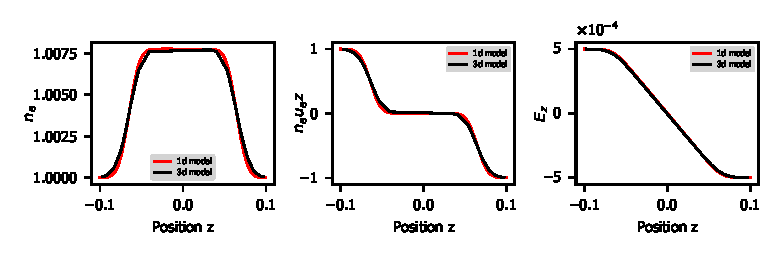
\includegraphics[scale=1.2]{z_axis_reduction.eps}
    \caption{Case I, $\lambda = 1$: Comparison of 1D two-fluid model and of 3D results (at
      time $t = 5 \times 10^{-4}$ projected onto the $z$-axis. The simulations were both
      conducted on meshes with 64 cells along the $z$-axis. No friction terms were taken
      into account.}
    \label{fig:z_axis_reduction}
\end{figure}

\subsection{Case II: 3D Cylindrical Problem}

We stick to the setting in Section \ref{sec:BC} and use the following initial conditions
\begin{equation*}
    n_\ast(\mathbf{x}, 0) = 1, \ \ \  p_\ast(\mathbf{x},0) = 1, \ \ \forall \mathbf{x}\in\Omega, \ast \in \{e, i\}.
\end{equation*}
All the other variables are set to zero initially. We set $\varphi(\mathbf{x}, t)|_{\Gamma_C^-} = 0, \varphi(\mathbf{x}, t)|_{\Gamma_C^+} = 1$, that is, a constant voltage is applied at the anode and excites the system. 

The cylindrical domain is 5.0 in length and 1.5 in radius. The plasma domain $\Omega_P$ is
1.0 in radius, i.e. the non-conducting domain $\Omega_N$ has an inner radius of 1.0 and an
outer radius of 1.5.

\begin{remark}
  Such an initial state is compatible with the boundary conditions and the quasi-neutrality
  condition $\rho = 0$, which means no initial layer and boundary layer in the sense of
  perturbation theory will arise when $\lambda \rightarrow 0$.
\end{remark}

In Fig. \ref{fig:3d_vec_field_E_B_ue}, the numerical solutions for $\lambda = 1.0, 0.1$
and $0$ are shown to visualize the 3D structure of the electromagnetic field. Qualitative
verification can be done in many aspects. First, the rotational symmetry of the problem is
preserved. Second, the $\mathbf{E}$-field points from $\Gamma^+_C$ to $\Gamma^-_C$ with a
relatively uniform value of approximately 0.2
($=\text{applied voltage}/\text{cylinder length}$) as a consequence of the irrotational
$\mathbf{E}$-field in the steady state according to Faraday's law (, which is also confirmed
in Fig.~\ref{fig:stabilization_comparison} \textbf{(b)}). Note that it does not hold for $\lambda = 1$
since the system has a large characteristic time and takes a long time to reach an
equilibrium, as will be shown later in Fig. \ref{fig:origin-data_vs_time}. Besides, the
$\mathbf{B}$-field is azimuthal (vortex-shaped) and orthogonal to the
$\mathbf{E}$-field. Also, under the electric force, the electrons move towards the anode
$\Gamma^+_C$ as expected.
\begin{figure}
    \centering
    \begin{subfigure}[b]{\textwidth}
        \hspace{-1cm}
        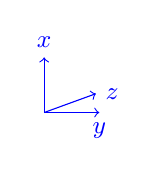
\begin{tikzpicture}
        \draw[blue, -to] (0,0) -- (20:0.7) node[right]{\small $z$};
        \draw[blue, -to] (0,0) -- (0,0.7) node[above]{\small $x$};
        \draw[blue, -to] (0,0) -- (0.7,0) node[below]{\small $y$};
        \end{tikzpicture}
        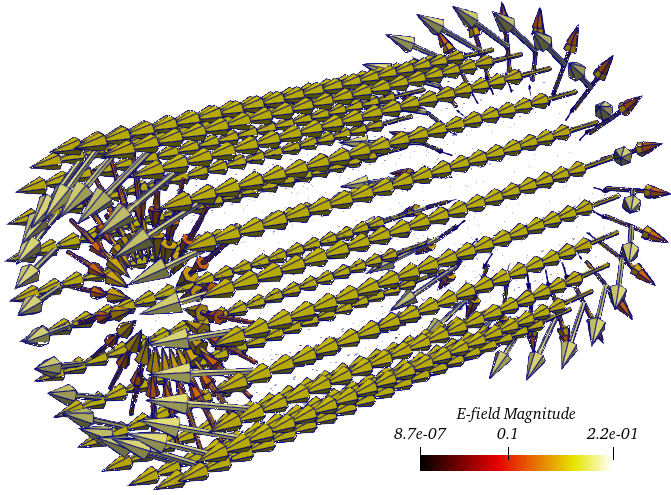
\includegraphics[scale=0.25]{E-field_lambda-1.png}
        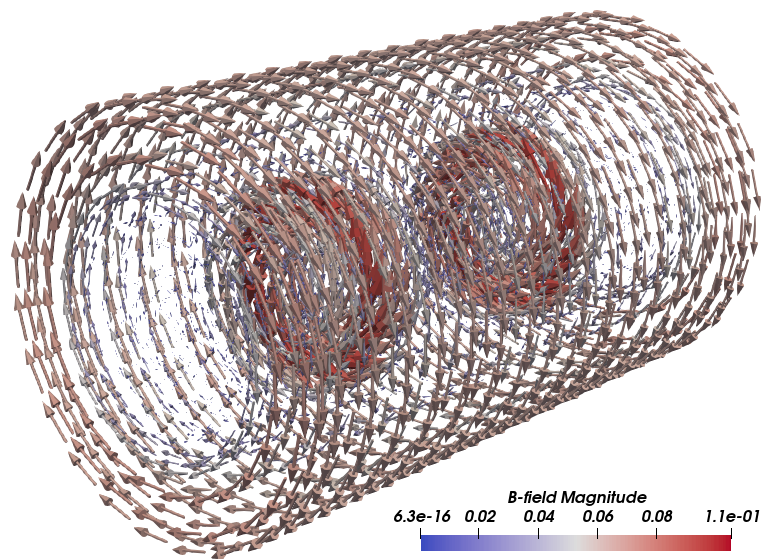
\includegraphics[scale=0.25]{B-field_lambda-1.png}
        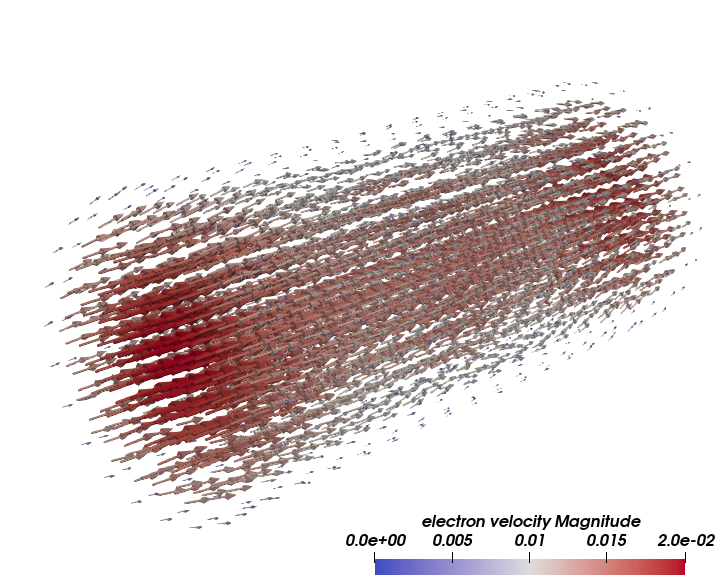
\includegraphics[scale=0.25]{electronVel_lambda-1.png}
        \caption{\colorbox{yellow!30}{$\lambda = 1.0$}}
    \end{subfigure}
     \begin{subfigure}[b]{\textwidth}
        \hspace{-1cm}
        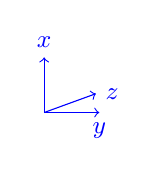
\begin{tikzpicture}
        \draw[blue, -to] (0,0) -- (20:0.7) node[right]{\small $z$};
        \draw[blue, -to] (0,0) -- (0,0.7) node[above]{\small $x$};
        \draw[blue, -to] (0,0) -- (0.7,0) node[below]{\small $y$};
        \end{tikzpicture}
        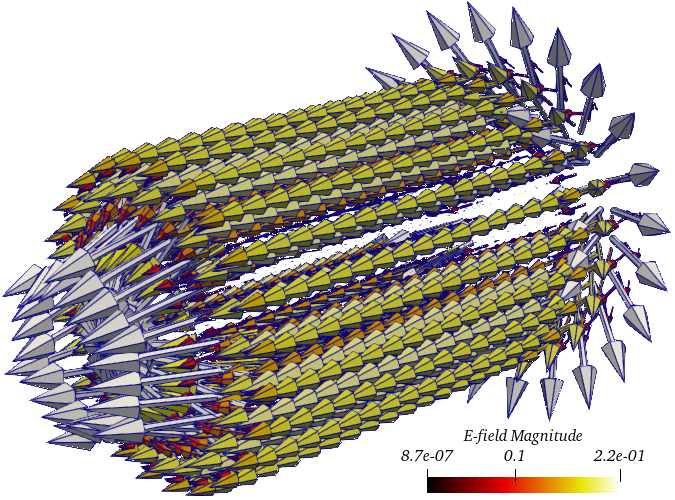
\includegraphics[scale=0.25]{E-field_lambda-1e-1.png}
        \hspace{0.3cm}
        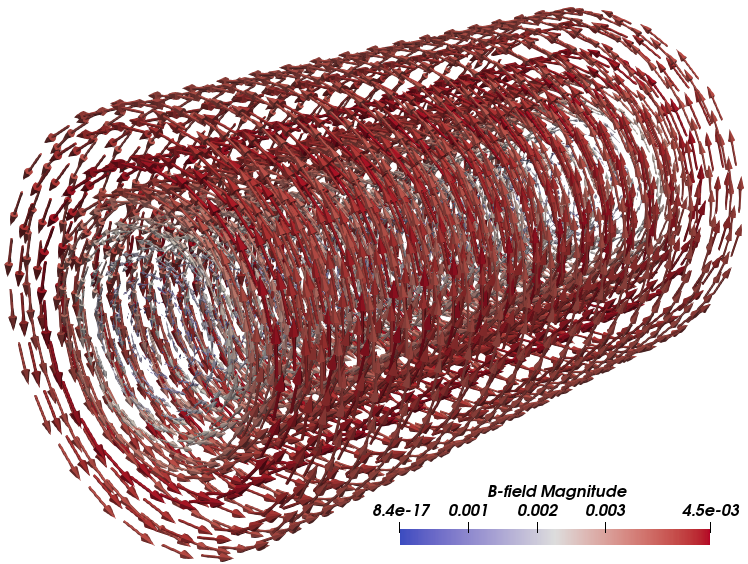
\includegraphics[scale=0.25]{B-field_lambda-1e-1.png}
        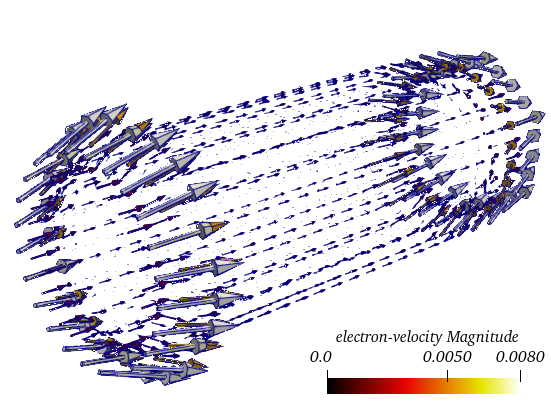
\includegraphics[scale=0.25]{electronVel_lambda-1e-1.png}
        \caption{\colorbox{yellow!30}{$\lambda = 0.1$}}
    \end{subfigure}
    \begin{subfigure}[b]{\textwidth}
        \hspace{-1cm}
        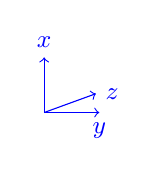
\begin{tikzpicture}
        \draw[blue, -to] (0,0) -- (20:0.7) node[right]{\small $z$};
        \draw[blue, -to] (0,0) -- (0,0.7) node[above]{\small $x$};
        \draw[blue, -to] (0,0) -- (0.7,0) node[below]{\small $y$};
        \end{tikzpicture}
        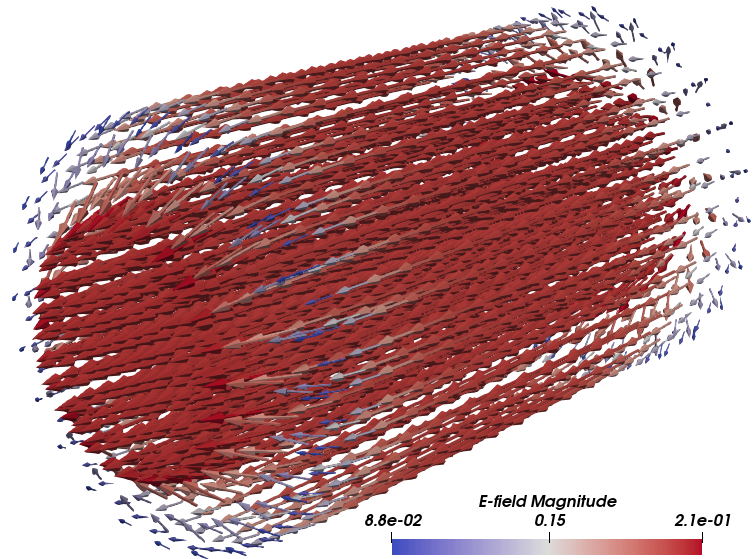
\includegraphics[scale=0.25]{E-field_lambda-0.png}
        \hspace{0.3cm}
        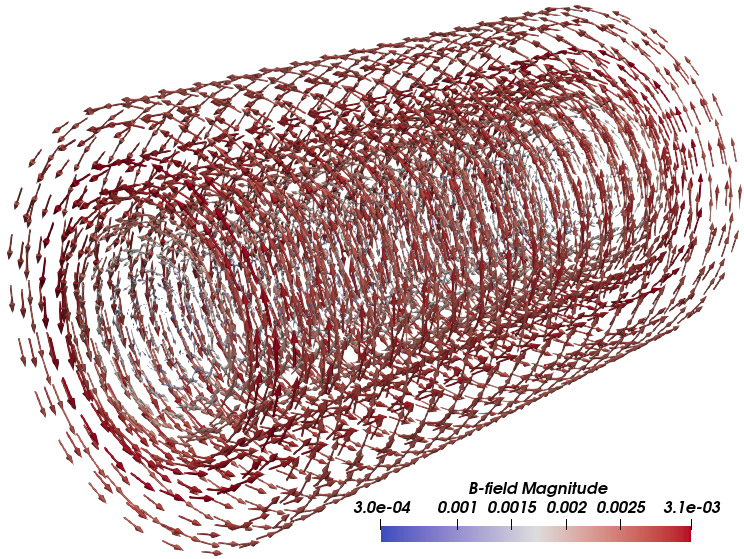
\includegraphics[scale=0.25]{B-field_lambda-0.png}
        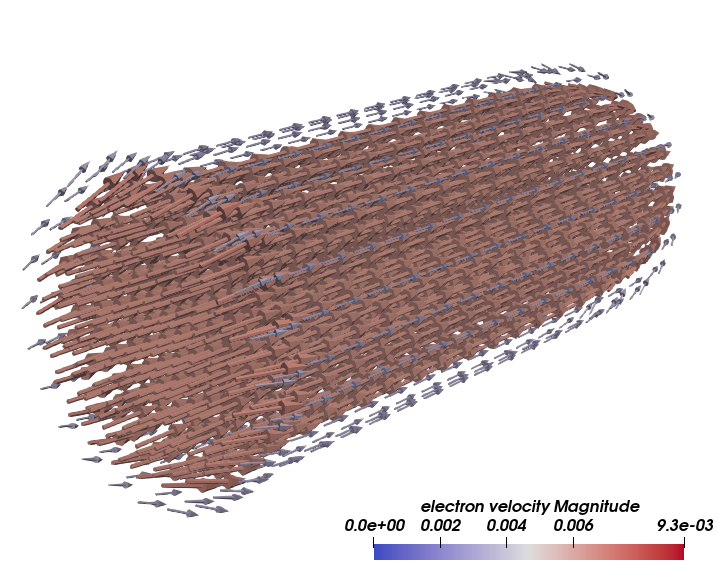
\includegraphics[scale=0.25]{electronVel_lambda-0.png}
        \caption{\colorbox{yellow!30}{$\lambda = 0.0$}}
    \end{subfigure}
    \caption{Case II: Snapshots of the $\mathbf{E}$-field, $\mathbf{B}$-field, and $\mathbf{u}_e$ for different $\lambda$ at $t = 10$ based on a primal mesh with 1920 cells (16 cells along $z$-axis). } 
    \label{fig:3d_vec_field_E_B_ue}
\end{figure}

Next, we study the impact of mesh refinement. Due to the high computational cost in 3D
simulations, reference solutions produced by a highly-refined mesh are not
available. Therefore, we demonstrate results generated by relatively coarse
meshes. Tab.~\ref{tab:grid_study_norm} lists $L^2$-norms of the solutions on different
meshes, which indicates robustness with respect to mesh refinement. To reveal more
features of the solutions, in Fig.~\ref{fig:grid_study_3d_clip_lambda-1e-1} (for
$\lambda = 0.1$) and Fig.~\ref{fig:grid_study_3d_clip_lambda-0} (for $\lambda = 0$) we plot
cross-section a the same locations for solutions produced on different meshes. Reasonable
qualitative agreement is observed. 

\begin{table}[]
    \centering
    \begin{tabular}{c | c c c | c c c}
        \hline\hline
        \multirow{2}{1em}{$N_V$} & \multicolumn{3}{c|}{\colorbox{yellow!30}{$\lambda = 1$}}
        &
        \multicolumn{3}{c}{\colorbox{yellow!30}{$\lambda = 0$}} \\
        \cline{2-4} \cline{5-7}
        & $\|n_e \|_{L^2}$ & $\|\mathbf{E} \|_{L^2}$ & $\|\mathbf{B} \|_{L^2}$ & $\|n_e
        \|_{L^2}$
        & $\|\mathbf{E} \|_{L^2}$ & $\|\mathbf{B} \|_{L^2}$  \\
        \hline
         1920  &  4.40 & 0.466 & 0.214 & 4.40 & 1.14 & 0.0155 \\
         3840  &  4.40 & 0.443 & 0.208 & 4.40 & 1.14 & 0.0155 \\
         14592 &  3.84 & 0.381 & 0.256 & 3.84 & 1.14 & 0.0135 \\ 
         29184 &  3.84 & 0.362 & 0.256 & 3.84 & 1.14 & 0.0135 \\
         \hline\hline
    \end{tabular}
    \caption{$L^2$-norms of the electron density, the $\mathbf{E}$-field and the
      $\mathbf{B}$-field on meshes of different size when
      \colorbox{yellow!30}{$\lambda = 1$} or $\lambda = 0$.}
    \label{tab:grid_study_norm}
\end{table}

\begin{figure}
    \centering
    \begin{minipage}{0.0\textwidth}
    \Large
    \vspace{0.4cm}
    $\mathbf{|E|}$
    
    \vspace{2.2cm}
    $\mathbf{|B|}$
    
    \vspace{2.2cm}
    $n_e$
    
    \vspace{1.9cm}
    $n_i$
    \end{minipage}
    \begin{minipage}{0.9\textwidth}
    \centering
    \textit{\textsf{Refinement 1\hspace{2.5cm}Refinement 2\hspace{2.5cm}Refinement 3\hspace{1cm}}}
    
    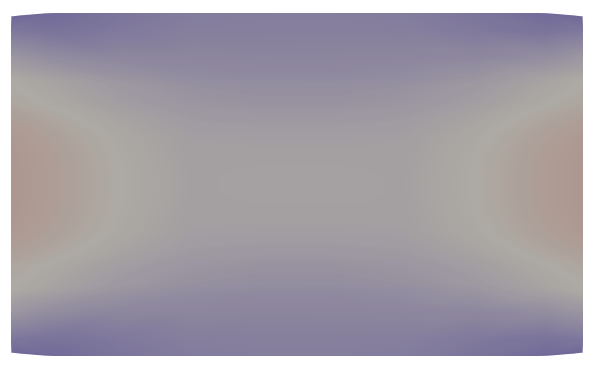
\includegraphics[scale=0.27]{clip_E_T-1_lambda-1e-1_8-2-2.png}
    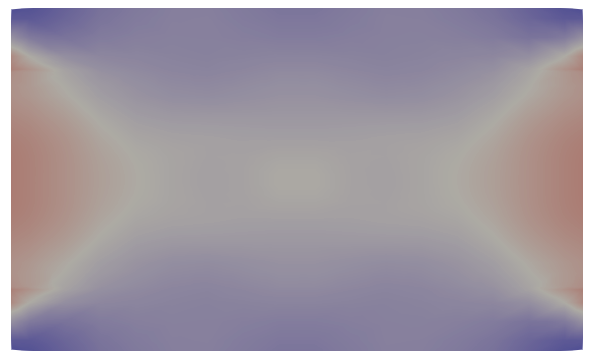
\includegraphics[scale=0.27]{clip_E_T-1_lambda-1e-1_16-3-3.png}
    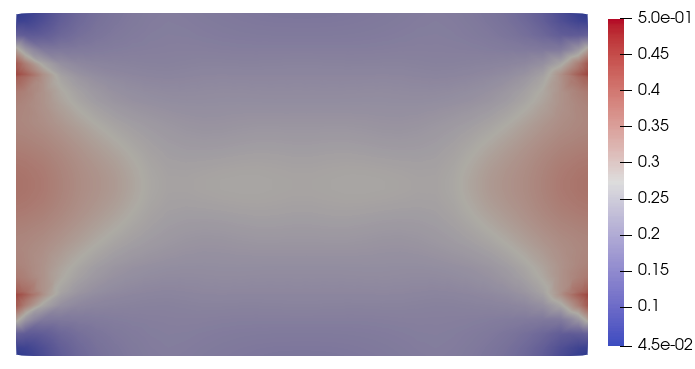
\includegraphics[scale=0.27]{clip_E_T-1_lambda-1e-1_32-3-4.png}
    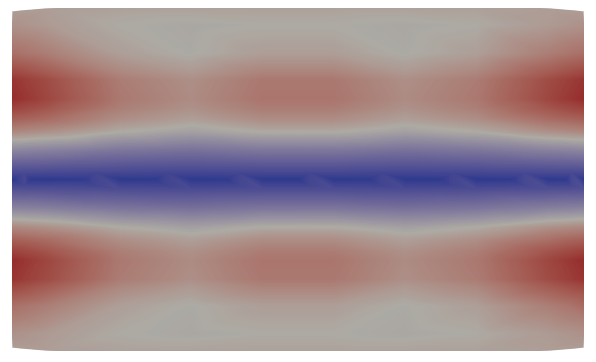
\includegraphics[scale=0.27]{clip_B_T-1_lambda-1e-1_8-2-2.png}
    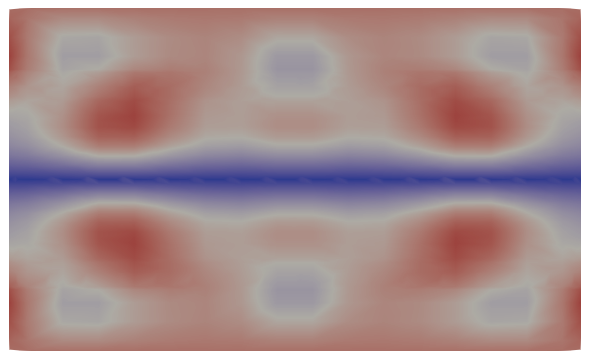
\includegraphics[scale=0.27]{clip_B_T-1_lambda-1e-1_16-3-3.png}
    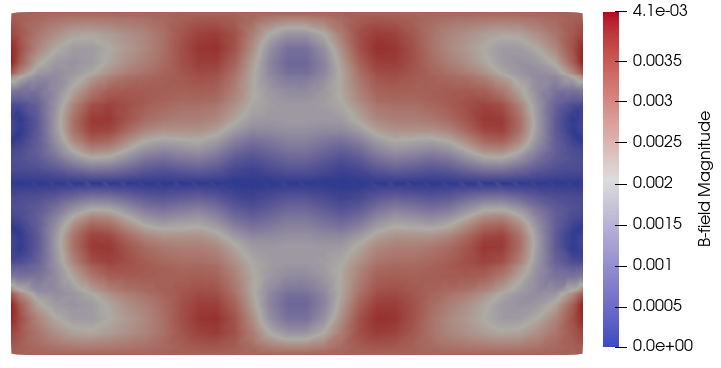
\includegraphics[scale=0.27]{clip_B_T-1_lambda-1e-1_32-3-4.png}
    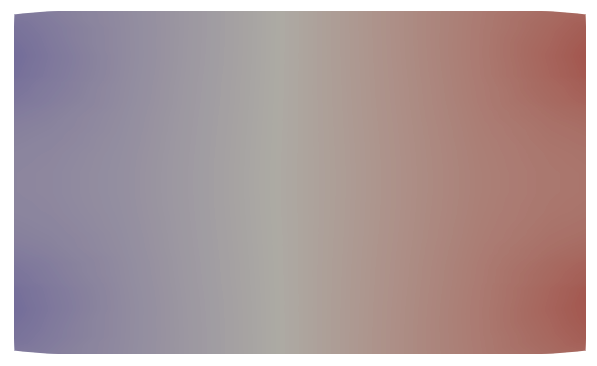
\includegraphics[scale=0.27]{clip_ne_T-1_lambda-1e-1_8-2-2.png}
    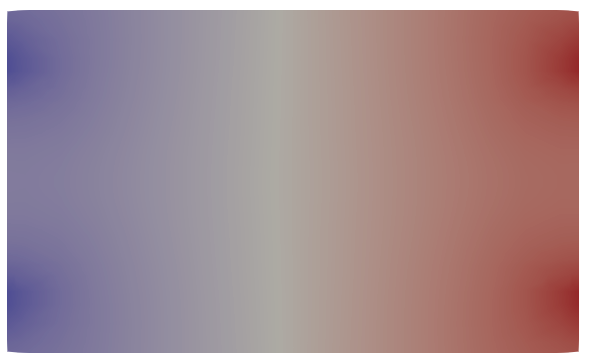
\includegraphics[scale=0.27]{clip_ne_T-1_lambda-1e-1_16-3-3.png}
    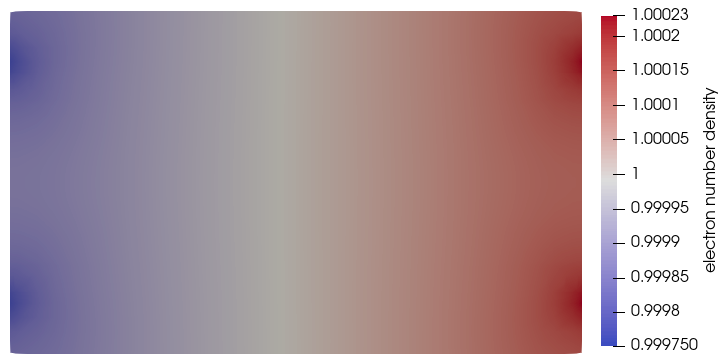
\includegraphics[scale=0.27]{clip_ne_T-1_lambda-1e-1_32-3-4.png}
    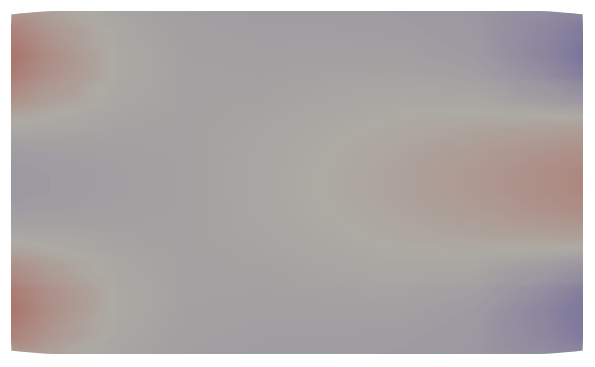
\includegraphics[scale=0.27]{clip_ni_T-1_lambda-1e-1_8-2-2.png}
    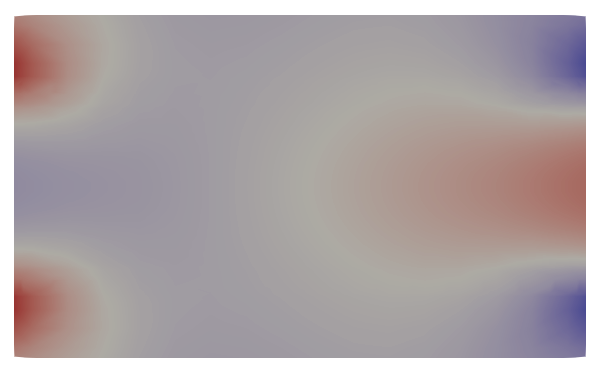
\includegraphics[scale=0.27]{clip_ni_T-1_lambda-1e-1_16-3-3.png}
    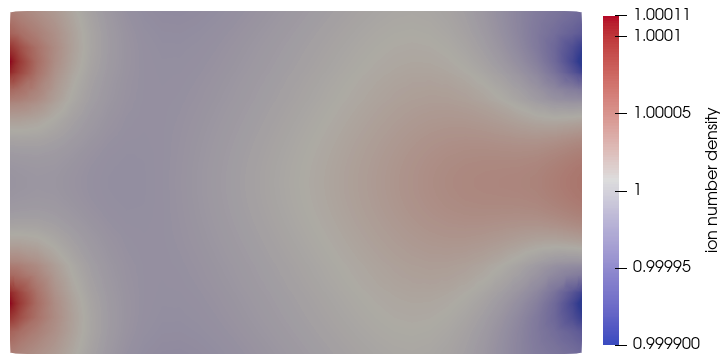
\includegraphics[scale=0.27]{clip_ni_T-1_lambda-1e-1_32-3-4.png}
    \end{minipage}
    \caption{Case II: Computed quantities at a cross-section on meshes with different
      refinement levels: 1920 primal cells in Refinement 1; 14592 primal cells in
      Refinement 2; 30720 primal cells in refinement 3. The snapshots are computed for
      \colorbox{yellow!30}{$\lambda = 0.1$} at $t = 1$.}
    \label{fig:grid_study_3d_clip_lambda-1e-1}
\end{figure}

\begin{figure}
    \centering
    \begin{minipage}{0.0\textwidth}
    \Large
    \vspace{0.4cm}
    $\mathbf{|E|}$
    
    \vspace{2.2cm}
    $\mathbf{|B|}$
    
    \vspace{2.2cm}
    $n_e$
    
    \vspace{1.9cm}
    $n_i$
    \end{minipage}
    \begin{minipage}{0.9\textwidth}
    \centering
    \textit{\textsf{Refinement 1\hspace{2.5cm}Refinement 2\hspace{2.5cm}Refinement 3\hspace{1cm}}}
    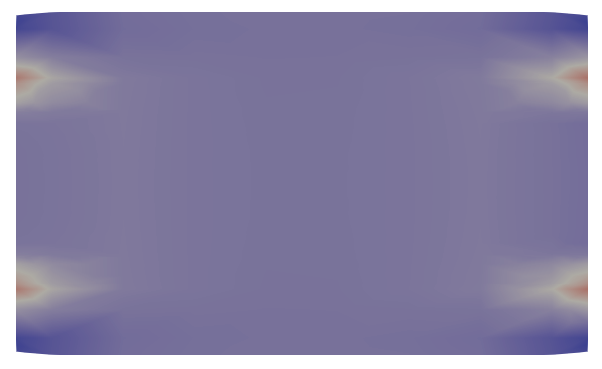
\includegraphics[scale=0.27]{slice_E_T-1_lambda-0_8-2-2.png}
    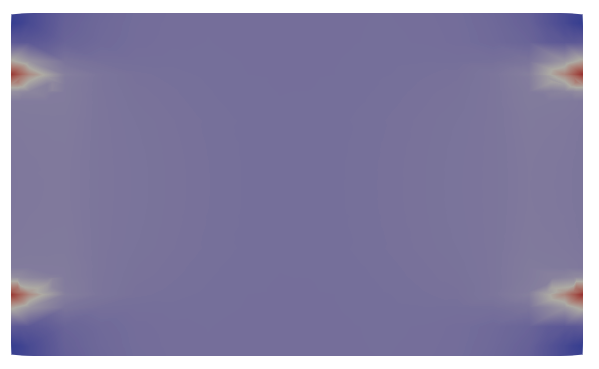
\includegraphics[scale=0.27]{slice_E_T-1_lambda-0_16-3-3.png}
    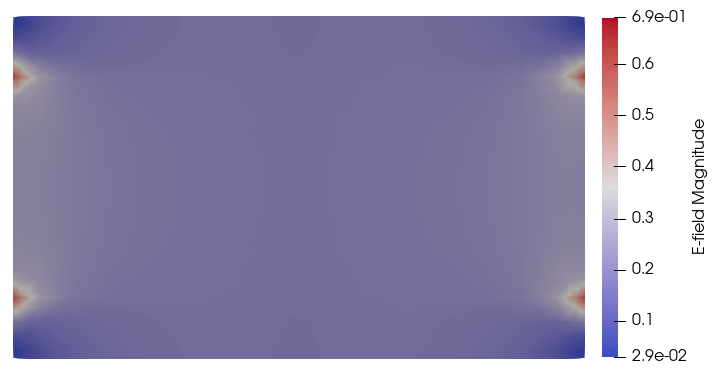
\includegraphics[scale=0.27]{slice_E_T-1_lambda-0_32-3-4.png}
    
    \hspace{0.0cm}
    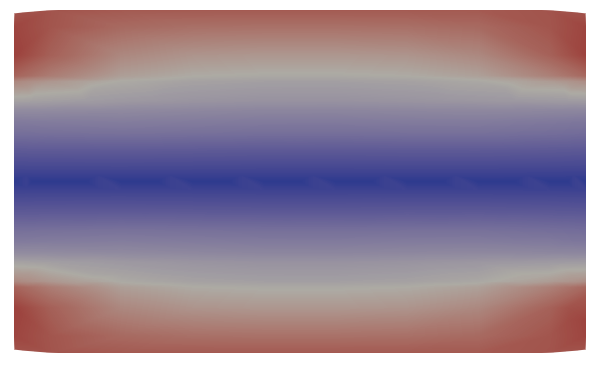
\includegraphics[scale=0.27]{slice_B_T-1_lambda-0_8-2-2.png}\hspace{0.02cm}
    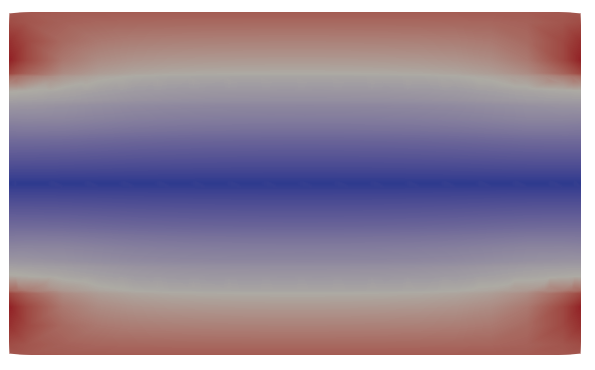
\includegraphics[scale=0.27]{slice_B_T-1_lambda-0_16-3-3.png}\hspace{0.02cm}
    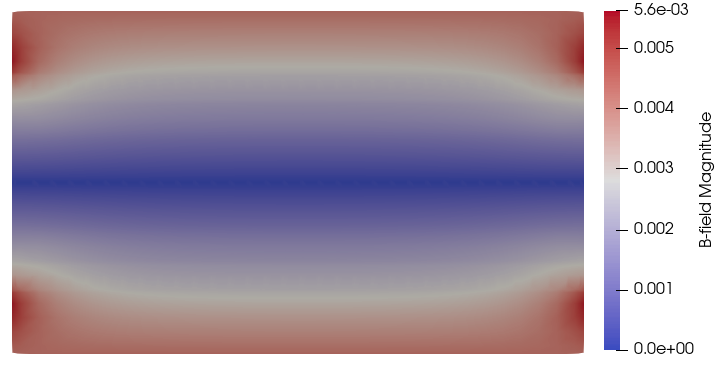
\includegraphics[scale=0.27]{slice_B_T-1_lambda-0_32-3-4.png}
    
    \hspace{0.04cm}
    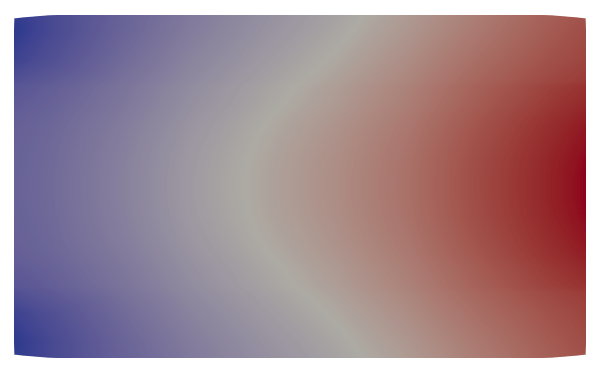
\includegraphics[scale=0.27]{slice_ne_T-1_lambda-0_8-2-2.png}\hspace{0.04cm}
    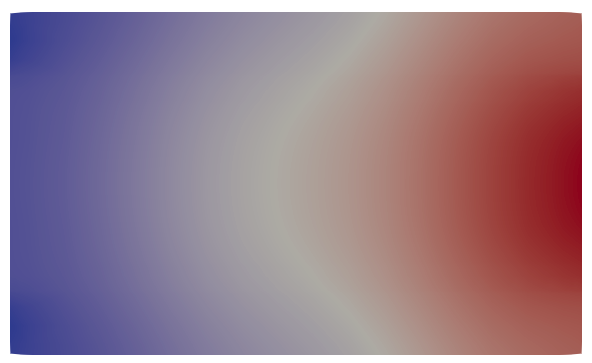
\includegraphics[scale=0.27]{slice_ne_T-1_lambda-0_16-3-3.png}\hspace{0.03cm}
    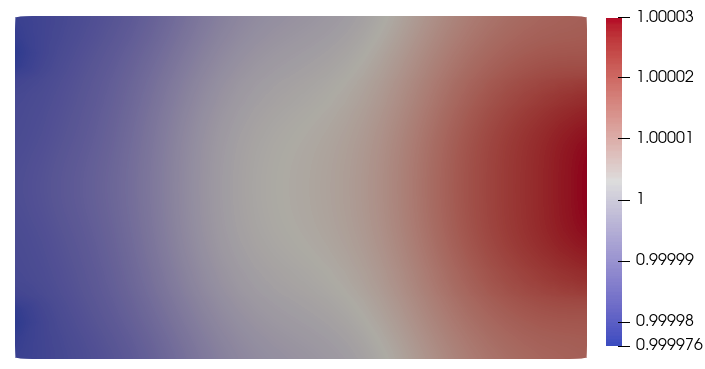
\includegraphics[scale=0.27]{slice_ne_T-1_lambda-0_32-3-4.png}
    
    \hspace{0.04cm}
    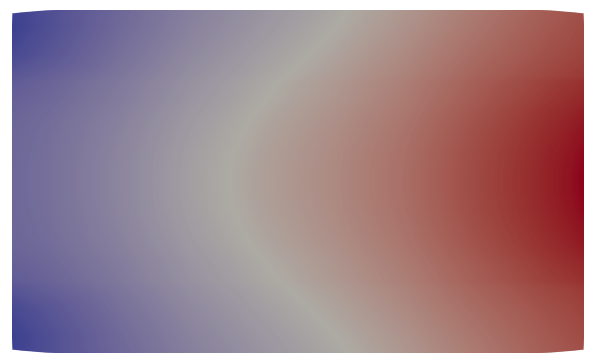
\includegraphics[scale=0.27]{slice_ni_T-1_lambda-0_8-2-2.png}\hspace{0.04cm}
    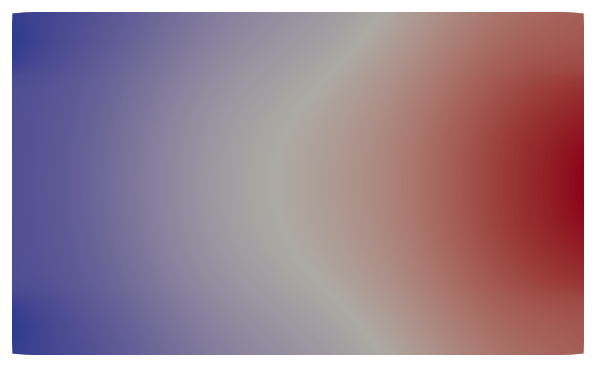
\includegraphics[scale=0.27]{slice_ni_T-1_lambda-0_16-3-3.png}\hspace{0.04cm}
    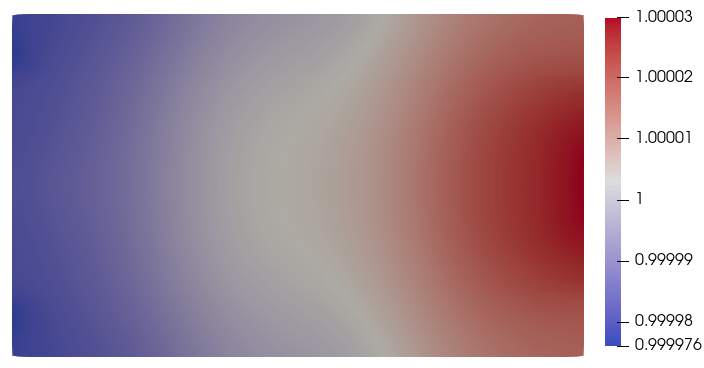
\includegraphics[scale=0.27]{slice_ni_T-1_lambda-0_32-3-4.png}
    \end{minipage}
    
    \caption{Case II: Computed quantities at a cross-section on meshes on different
      refinement levels. Refinement 1: 1920 primal cells; Refinement 2: 14592 primal
      cells; Refinement 3: 30720 primal cells. The snapshots are computed for
      \colorbox{yellow!30}{$\lambda = 0$} at $t = 1$.}
    \label{fig:grid_study_3d_clip_lambda-0}
\end{figure}

To inspect how the system evolves, the time histories of some quantities are displayed in
Fig.~\ref{fig:origin-data_vs_time}. Being in stable equilibrium at $t=0$, the system is
excited by applying a voltage and this triggers oscillations that decay over time. A
larger value of $\lambda$ leads to oscillations with larger amplitude and slower damping,
whereas for a smaller $\lambda$ the system quickly reaches a steady state. It is
consistent with the fact that $\lambda$ characterizes the time scale of the
electromagnetic field. From a different perspective, it is a reflection of the shielding
effect of the plasma which is characterized by the Debye length. Besides, the electrons
move much faster and oscillate more than ions as a consequence of the large difference in
inertia. Furthermore, the structure-preserving property of our scheme is revealed by the
exact balance of the currents at $\Gamma^+_C$ and $\Gamma^-_C$ \cite{Hiptmair_2021}, as is
shown in the bottom plot in Fig.~\ref{fig:origin-data_vs_time}.

\begin{figure}
  \centering
    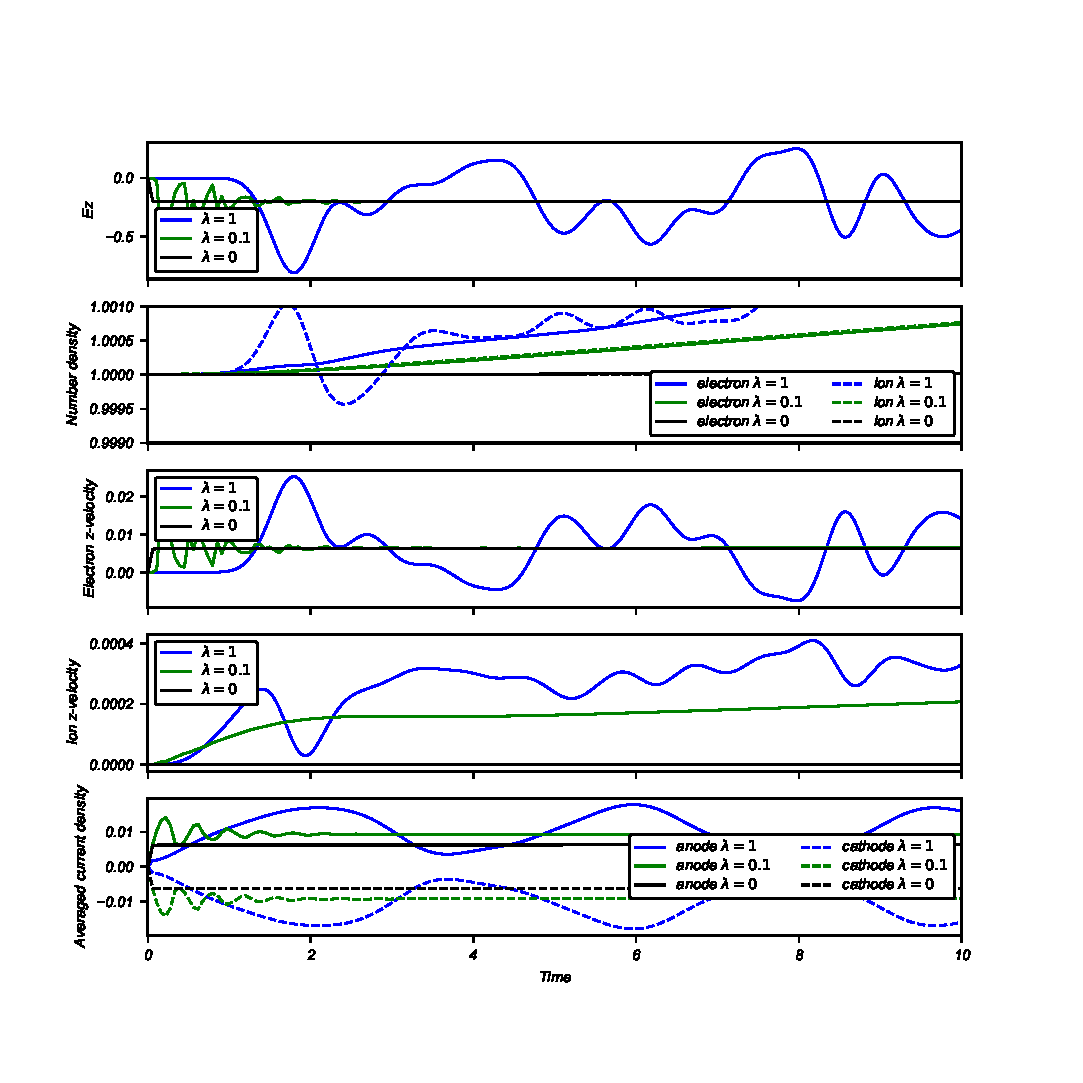
\includegraphics[scale=0.9]{data-vs-time_stepVoltage.eps}
    \caption{Case II: Time histories of quantities at the domain center and of the averaged current densities at $\Gamma^+_C$ (anode) and $\Gamma^-_C$ (cathode) for different values of $\lambda$. The simulations are done on a mesh with 1920 primal cells with 8 layers along the $z$-axis.}
    \label{fig:origin-data_vs_time}
\end{figure}

The stabilization proposed in Section \ref{sec:reform-discrete} is essential to achieve
good results when $\lambda$ tends to zero. As is shown in
Fig.~\ref{fig:stabilization_comparison} \textbf{(a)}, the scheme without stabilization incurs a blow-up
when $\lambda$ is close to zero. The proposed stabilization clearly offers a remedy.
\begin{figure}
    \centering
\begin{minipage}[t]{0.4\textwidth}\centering
  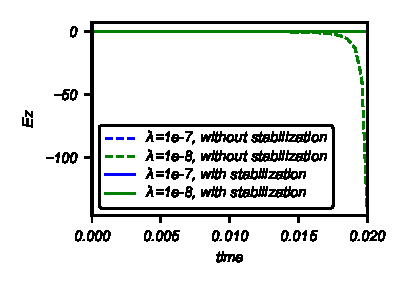
\includegraphics[width=\textwidth]{stabilizationComparision_stepVoltage.eps}

  \parbox{0.9\textwidth}{\begin{tabular}[c]{ll}
    \textbf{(a)} & time-dependent z-component of \\ & the $\mathbf{E}$-field
    in a boundary cell on $\Omega_N$
  \end{tabular}}
\end{minipage}%    
 \begin{minipage}[t]{0.6\textwidth}\centering
   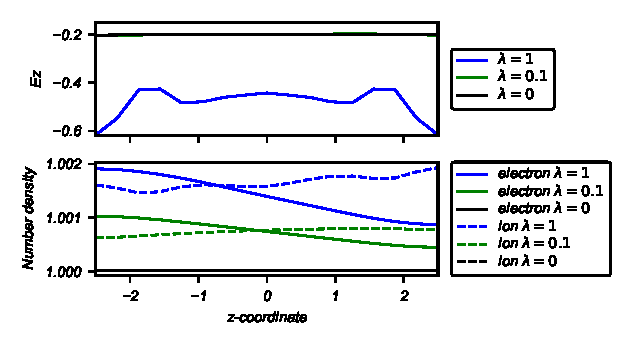
\includegraphics[width=\textwidth]{data-vs-z_stepVoltage.eps}

   \parbox{0.9\textwidth}{\begin{tabular}[c]{ll}
     \textbf{(b)} & Quantities along $z$-axis for different $\lambda$; the results \\ & 
     are computed at $t = 10$ on a mesh with 1920 primal  \\ &  cells and 8 layers along $z$-axis.
   \end{tabular}}
\end{minipage}%

\caption{Case II: \textbf{(a)} Stabilization in the non-conducting domain $\Omega_N$,
  \textbf{(b)} Numerical quasi-neutrality    }
\label{fig:stabilization_comparison}
\end{figure}

The capability of our approach to deal with the non-neutral ($\lambda = \mathcal{O}(1)$)
and quasi-neutral ($\lambda = 0$) regimes manifests itself in the reported numerical tests
in that valid results are produced for different values of $\lambda$ including
$\lambda=0$. It is instructive to verify the quasi-neutrality condition
(\ref{equ:maxwell_gauss_D_limit}) when $\lambda = 0$. To that end we display the
$\mathbf{E}$-field and particle densities on the $z$-axis in
Fig.~\ref{fig:stabilization_comparison} \textbf{(b)}. The bottom plot demonstrates that
the density profiles of the electrons and ions offset each other also for computed quantities:
Quasi-neutrality holds on the discrete level.

\section{Conclusion}

We have developed an AP scheme for the Euler-Maxwell plasma model in three spatial
dimensions that is applicable in both non-neutral $\lambda = \mathcal{O}(1)$ and
quasi-neutral $\lambda \rightarrow 0$ regimes. The main features of our work lie in: (i)
Maxwell's equations are discretized on primal and dual meshes by FIT (in the spirit of
DEC). By discretizing the Euler equations by FVM on the dual mesh, the coupling of two systems
is naturally realized via the connection of the mass flux and the electric current at each
dual face. (ii) A non-conducting region is taken into account where additional
stabilization is essential when $\lambda \rightarrow 0$. We enforce the vanishing
divergence of the $\mathbf{D}$-field through a Lagrange multiplier for any value of
$\lambda$. (iii) The alignment of primal-dual meshes at the boundary entails cut-off cells
and auxiliary unknowns have to be introduced. iv) A lumping trick is applied to the
conductivity matrix (relating the electric current and the electric field) to enhance
stability.

Our approach has been tested on a cylindrical domain with settings meant for electric arc
simulations. The AP property has been verified numerically. To the best of the authors'
knowledge, this work is among the first to try to solve the 3D fluid plasma model on
unstructured meshes, which potentially gives more flexibility than the
finite-difference-based approaches and reduces the computational cost compared to
particle-based approaches. In particular, the AP property allows us to address regimes
with vastly different Debye lengths.

\bibliography{ref}
\end{document}
%%% Local Variables:
%%% mode: latex
%%% TeX-master: t
%%% End:
